\documentclass[12pt, a4paper]{report}
\usepackage{newtxtext}
\usepackage{newtxmath}
\usepackage[utf8]{inputenc}
\usepackage[T1]{fontenc}   
\usepackage[brazilian]{babel}
\usepackage{graphicx}
\usepackage{chngcntr} 
\usepackage{hyperref}
\usepackage{float}
\usepackage{array}
\usepackage{booktabs}
\usepackage[
    top=3cm,
    bottom=2cm,
    left=3cm,
    right=2cm,
    a4paper
]{geometry}
\hypersetup{
    colorlinks=true,
    linkcolor=blue,
    filecolor=magenta,      
    urlcolor=blue,
    citecolor=blue,
}
\counterwithin{figure}{chapter}

\begin{document}

\title{Digitalização do Poder Judiciário: uma análise das políticas públicas de governo digital do CNJ com base nos índices de governo eletrônico internacionais} 

\author{Lázaro Damasceno}
\date{\today}
\maketitle

\listoffigures
\listoftables
\tableofcontents

\chapter{Referencial Teórico}

Para gerar os gráficos, fazer análises, determinar o valor e o método de correlação, fazer as tabelas e os mapas coropléticos, escolheu-se a linguagem de programação \textbf{Python}.

Foram usadas as bibliotecas \textbf{Pandas} para a análise exploratória de dados, \textbf{GeoPandas} para os mapas coropléticos, \textbf{Matplotlib} e \textbf{Seaborn} para a geração  de gráficos. Para a geração dos mapas foram usados os arquivos do projeto \textbf{Natural Earth} para os mapas do mundo e da malha municipal do Instituto Brasileiro de Geografia e Estatística. O tamanho das padronizado das figuras foi 10x6 polegadas, podendo ser utilizado outro, caso necessário.

Além dos argumentos anteriores, o coeficiente de correlação escolhido para todas as análises foi o de \textbf{Spearman}. \cite{hauke2011comparison} explica que o \textbf{coeficiente de correlação de Spearman} é uma estatística de postos não paramétrica (sem distribuição) proposta como uma medida da força da associação entre duas variáveis. É uma medida de uma associação monótona, usada quando a distribuição de dados torna o coeficiente de correlação de Pearson indesejável ou enganoso. 

Além disso, \cite{hauke2011comparison} esclarece que o \textbf{coeficiente de correlação de Spearman} não é uma medida da relação linear entre duas variáveis. Ele avalia quão bem uma função monotônica arbitrária pode descrever a relação entre duas variáveis, sem fazer quaisquer suposições sobre a distribuição de frequência das variáveis.

Ao contrário do \textbf{coeficiente de correlação de Pearson}, segundo \cite{hauke2011comparison}, ele não requer a suposição de que a relação entre as variáveis seja linear, nem requer que as variáveis sejam medidas em escalas intervalares; pode ser usado para variáveis medidas no nível ordinal.

Como forma de poder julgar qualquer valor de coeficiente de correlação encontrado, adotou-se a ideia de \cite{ali2022spearman}, presente na tabela \ref{tab:faixas-coeficiente-correlacao}.

\begin{longtable}[c]{@{}ll@{}}
	\caption{Faixas de coeficiente de correlação}
	\label{tab:faixas-coeficiente-correlacao}\\
	\toprule
	%
	\endfirsthead
	%
	\toprule
	%
	\endhead
	%
	\textbf{Faixa} & \textbf{Significado} \\ \midrule
	1           & Correlação positiva completa. \\ \midrule
	0,99 - 0,70 & Correlação positiva forte.    \\ \midrule
	0,5 - 0,69  & Correlação positiva média.    \\ \midrule
	0,1 - 0,49  & Correlação positiva fraca.    \\ \midrule
	0           & Sem relação positiva.         \\ \bottomrule
	\footnotesize{Fonte: elaboração baseada em \cite{ali2022spearman}.}
\end{longtable}

Para qualquer coeficiente de correlação, adotar-se-ão os critérios presentes na tabela \ref{tab:faixas-coeficiente-correlacao} para determinar a existência ou não de correlação entre as variáveis comparadas.

Para as análises de regressão, optou-se pela polinomial ao invés da tradicional regressão linear. Similar a comparação com os coeficientes de correlação entre \textbf{Pearson} e \textbf{Spearman}, como a abordagem da análise dos coeficientes de correlação descartou relações lineares entre as variáveis analisadas, a regressão polinomial se alinha a escolha do coeficiente de correlação.

Finalmente, as figuras usadas neste trabalho, os códigos dos notebooks \textbf{Jupyter} usados para gerar as figuras e as bases da dados estão acessíveis em \url{https://github.com/LazaroDamasceno/Dissertacao-Mestrado-PoderJud-EGDI}.
\chapter{E-Government Development Index}

\cite{martinez2022egovernment} cita 4 indicadores de governo eletrônico: EGDI da ONU, DESI da Comissão Europeia, DGI da OCDE e GTMI do Banco Mundial.

O DESI, conforme \cite{desi_2022}, a Comissão Europeia tem monitorado anualmente desde 2014 o progresso dos Estados-membros da União Europeia. Cada relatório anual inclui análises individualizadas que ajudam os Estados-membros a identificar ações prioritárias e capítulos temáticos, provendo análises de áreas de política pública digital.

Dos índices remanescentes, escolheu-se pela quantidade de citações dos EGDI, DGI e GTMI no Google Acadêmico.

\begin{figure}[H]
    \centering
    \caption{Quantidade de citações dos EGDI, DGI e GTMI no Google Acadêmico}
    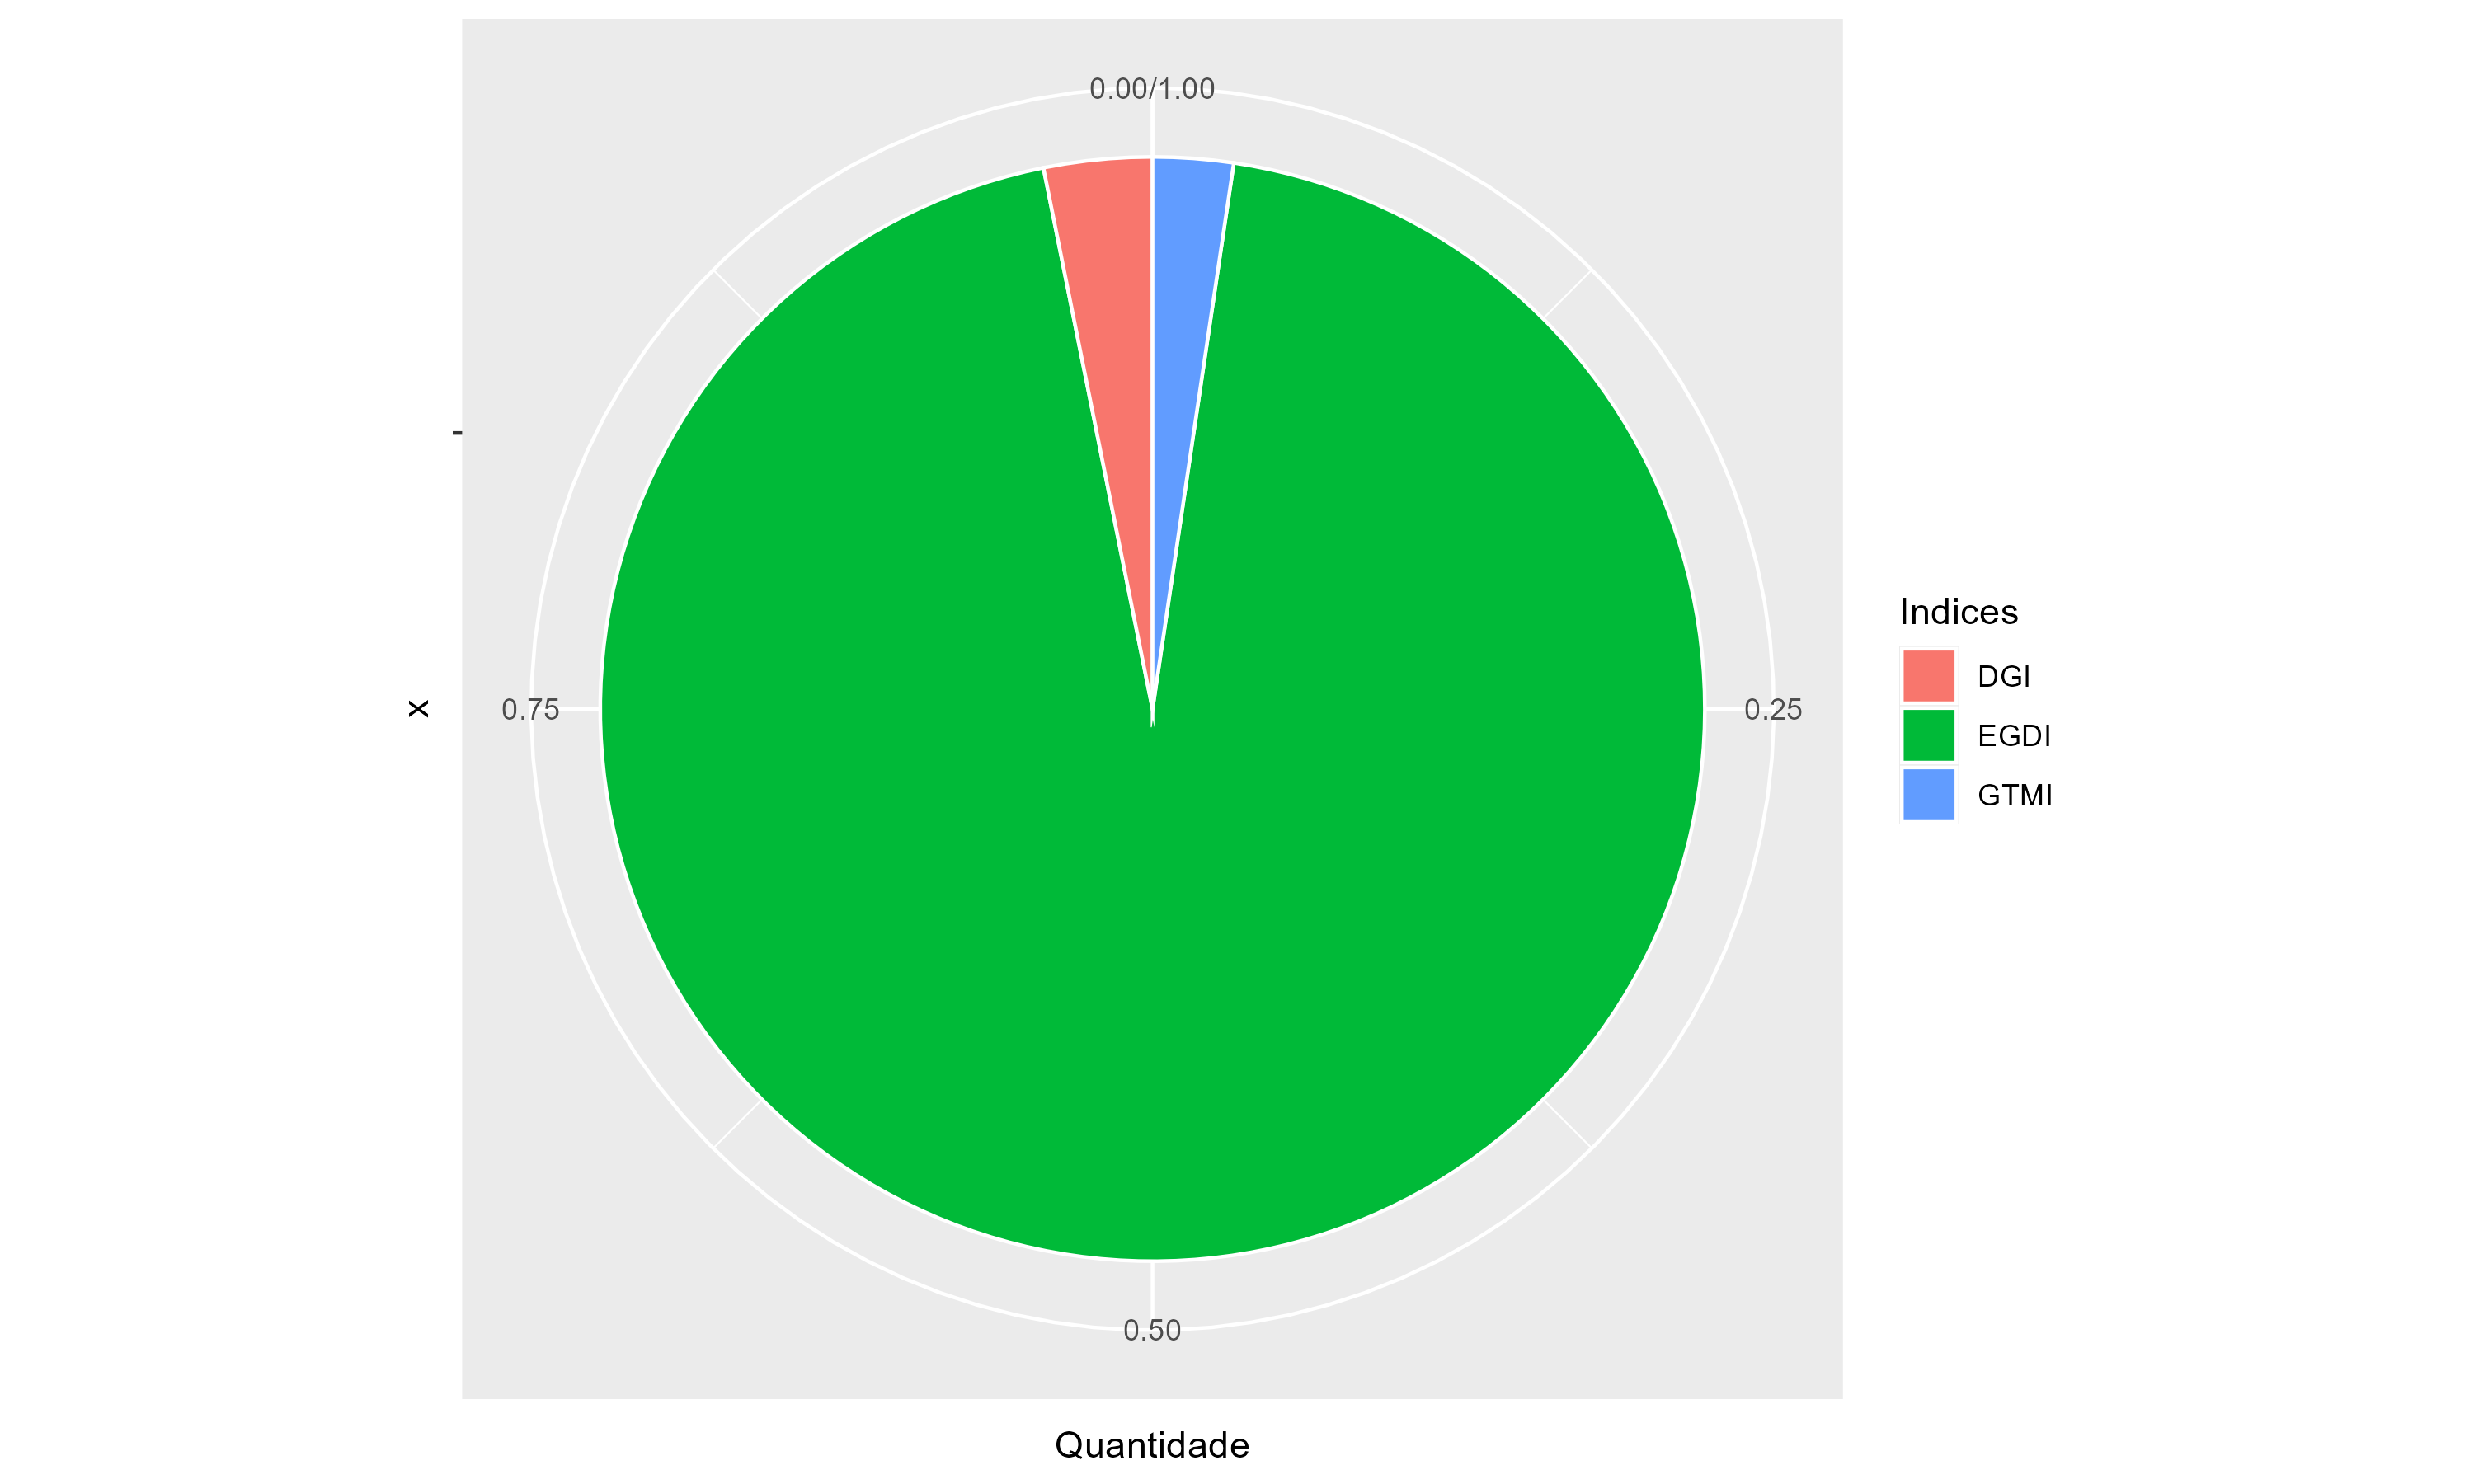
\includegraphics[width=1\linewidth]{figuras/egov_indices.png}
    \label{fig:egov_indices}
    \footnotesize{Fonte: elaboração própria.}
\end{figure}

Devido à quantidade massiva do EGDI, ele foi o escolhido. Para \cite{ONU_EGDI_description}, o EGDI apresenta o estado do desenvolvimento do governo eletrônico nos Estados-Membros das Nações Unidas.

Além de uma avaliação dos padrões de desenvolvimento de websites em um país, o EGDI incorpora as características de acesso, como infraestrutura e níveis educacionais, para refletir como um país está utilizando as tecnologias da informação para promover o acesso e a inclusão de sua população. 

\cite{ONU_EGDI_description} ainda acrescenta que o EGDI é uma medida composta por três importantes dimensões do governo eletrônico, a saber: prestação de serviços online, conectividade de telecomunicações e capacidade humana. 

A composição do EGDI é demonstrada pela figura \ref{fig:egdi_componentes}.

\begin{figure}[H]
    \centering
    \caption{Componentes do EGDI}
    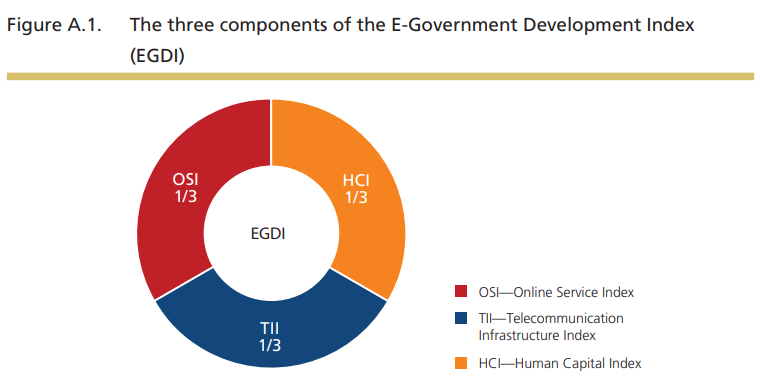
\includegraphics[width=1\linewidth]{figuras/egdi_componentes.png}
    \label{fig:egdi_componentes}
    \footnotesize{Fonte: \cite{ONU_EGDI_description}.}
\end{figure}

Além dos componentes OSI, TII e o HCI, há o EPI. \cite{ONU_EGDI_EPI_description} conceitua EPI como um índice suplementar derivado do EGDI. O índice de um país reflete os mecanismos de participação cidadã eletrônica que são empregados pelo poder público em comparação a todos os países.

Além disso, \cite{ONU_EGDI_EPI_description} argumenta que o propósito de medição do EPI não é prescrever nenhuma prática específica, mas sim oferecer entendimento de como os países estão usando ferramentas online para promover a interação entre o poder público e os cidadãos, e ainda entre o povo, para benefício coletivo.

A composição do EPI é, conforme \cite{ONU_EGDI_EPI_description}:

\begin{itemize}
    \item E-information: permitir a participação, fornecendo aos cidadãos informações públicas e acesso à informação sem ou mediante solicitação
    \item E-consultation: engajar os cidadãos em contribuição e deliberações sobre em políticas e serviços públicas.
    \item E-decision-making: empoderar os cidadãos via co-participação das políticas públicas e co-produção dos componentes dos serviços e as modalidades de entrega.
\end{itemize}

Considerando as informações anteriores, as figuras \ref{mapa_coropletico_paises_egdi}, \ref{mapa_coropletico_paises_epi}, \ref{mapa_coropletico_paises_hci}, \ref{mapa_coropletico_paises_hci} e \ref{mapa_coropletico_paises_tii} contêm mapas coropléticos que monstram o EGDI, seus componentes e o EPI pelo mundo.

\begin{figure}[H]
	\centering
	\caption{EGDI dos países do mundo em 2024}
	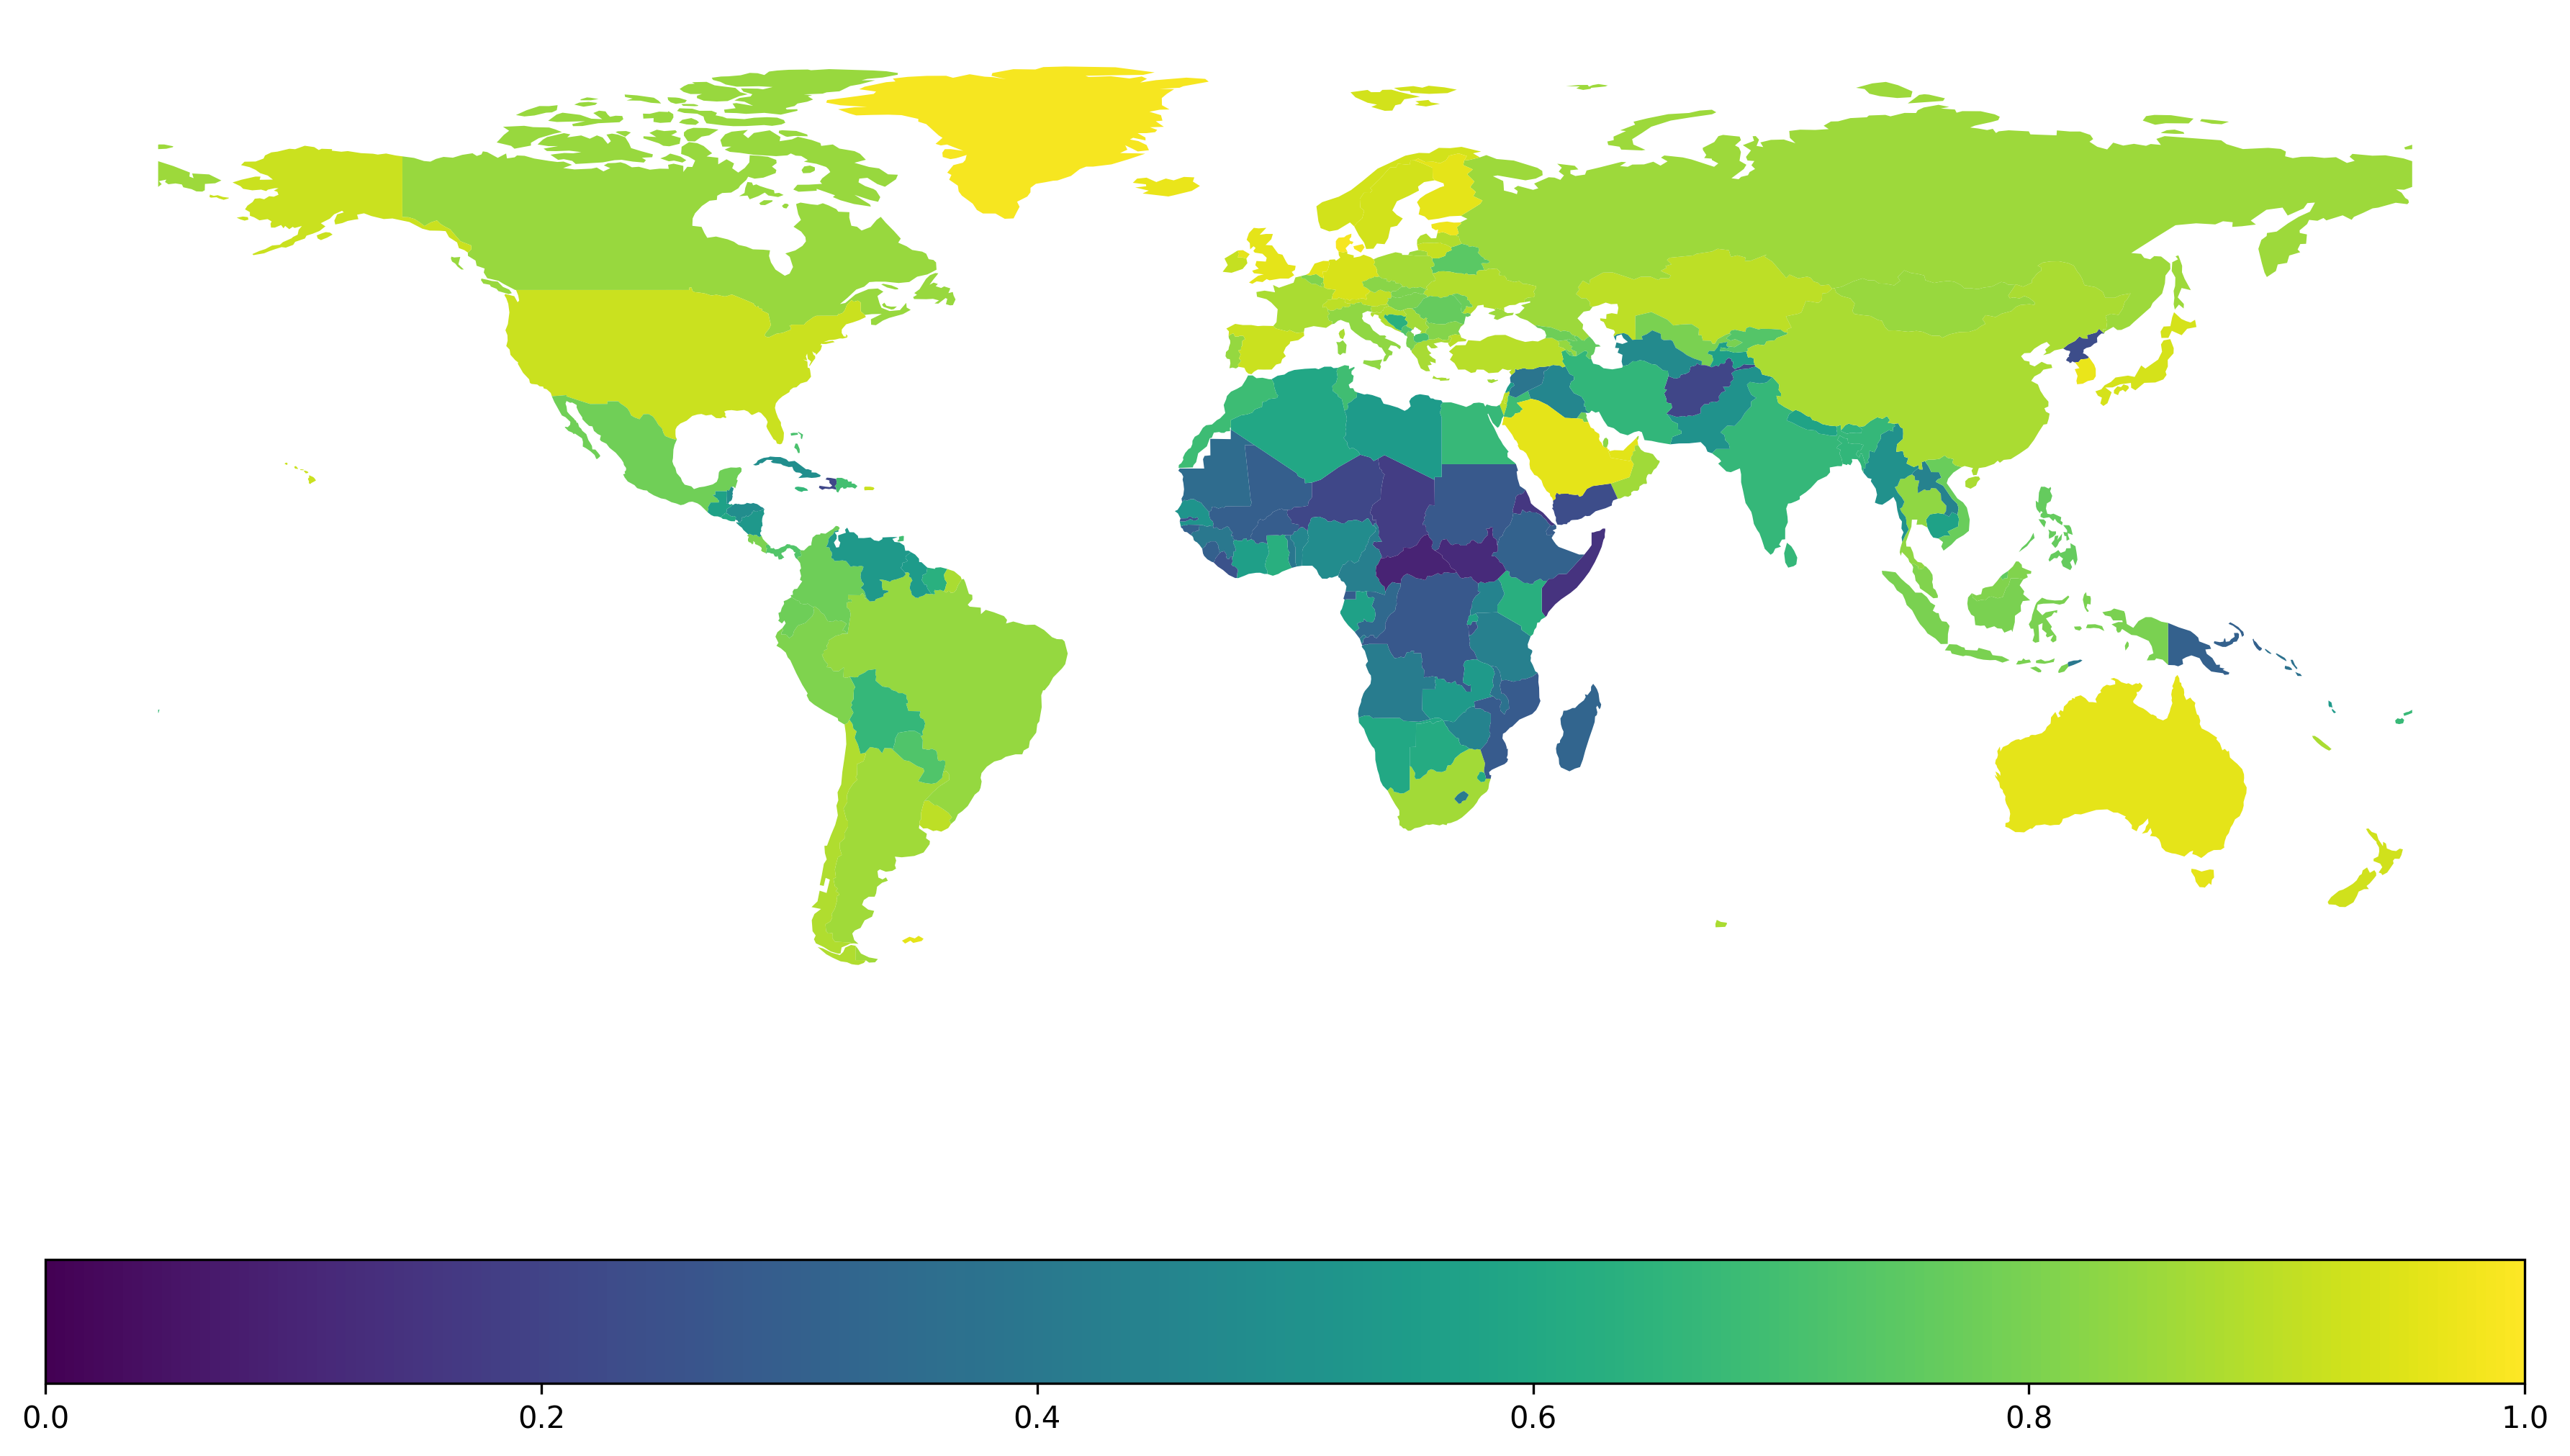
\includegraphics[width=1\linewidth]{figuras/mapa_coropletico_paises_egdi}
	\label{fig:mapa_coropletico_paises_egdi}
	\footnotesize{Fonte: elaboração própria baseada em \cite{ONU_EGDI_mapa}.}
\end{figure}

\begin{figure}[H]
	\centering
	\caption{EPI dos países do mundo em 2024}
	
\includegraphics[width=1\linewidth]{figuras/mapa_coropletico_paises_epi}
	\label{fig:mapa_coropletico_paises_epi}
	\footnotesize{Fonte: elaboração própria baseada em \cite{ONU_EGDI_mapa}.}
\end{figure}

\begin{figure}[H]
	\centering
	\caption{HCI dos países do mundo em 2024}
	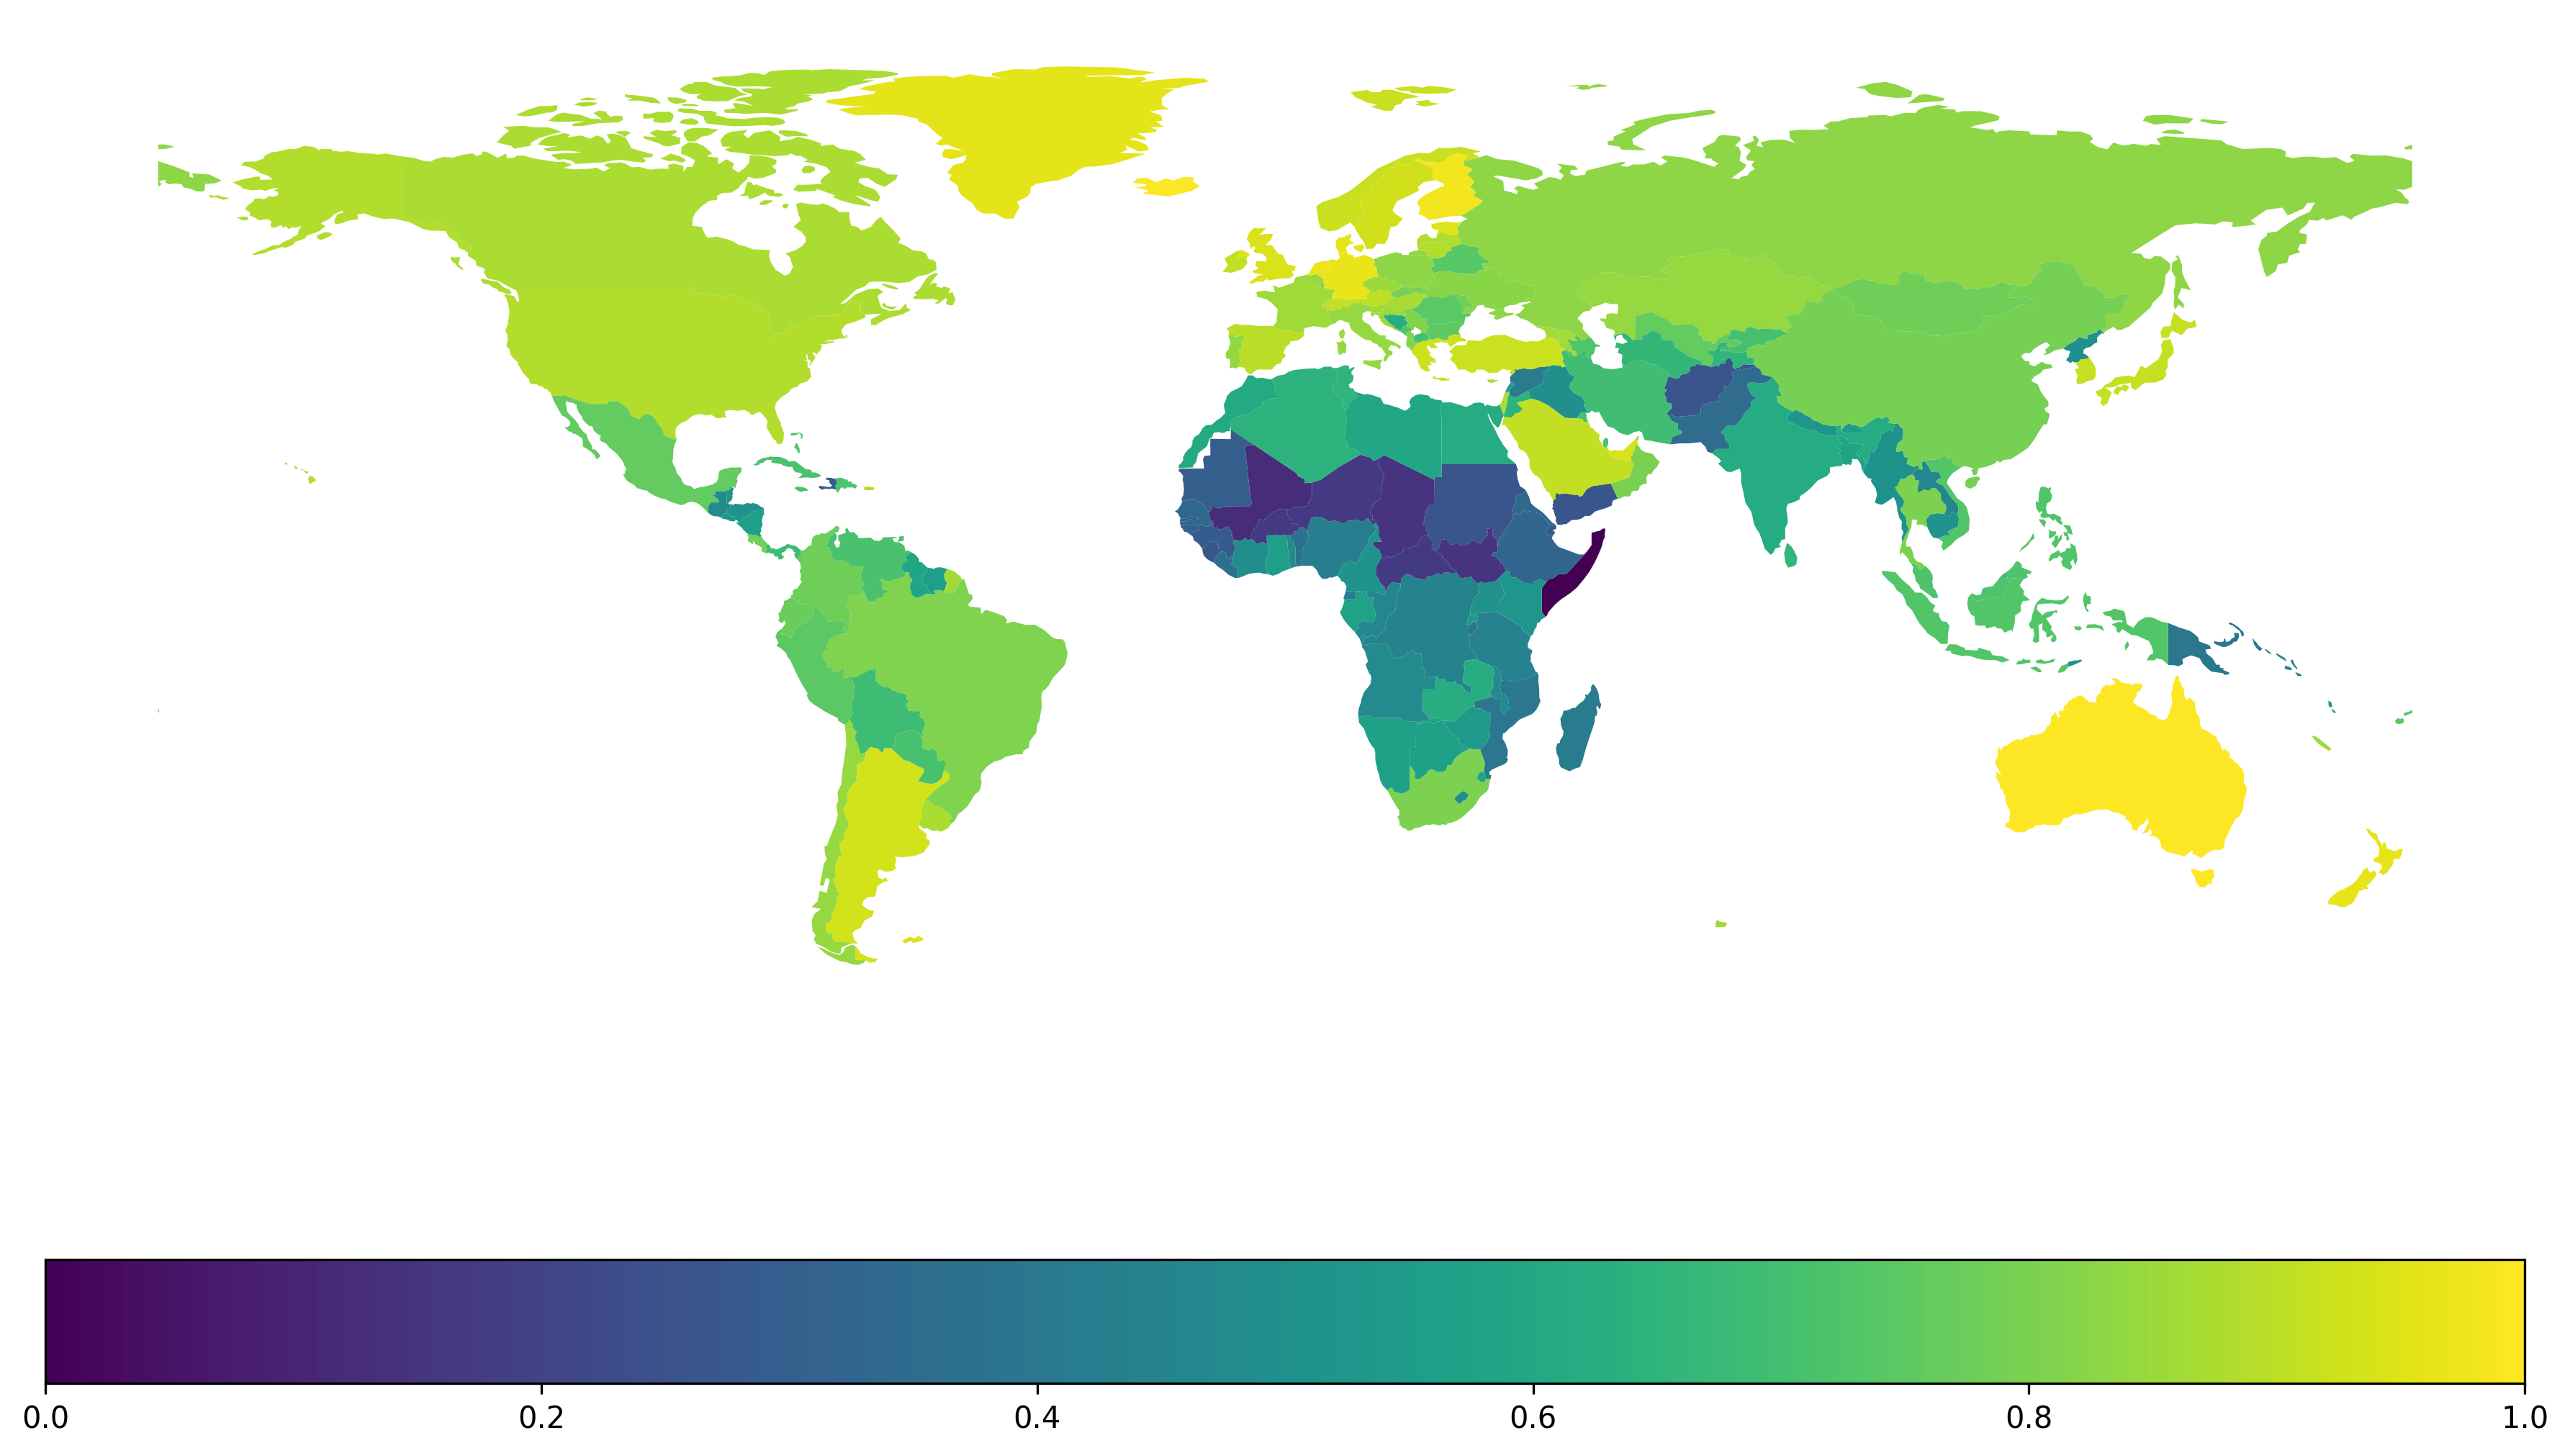
\includegraphics[width=1\linewidth]{figuras/mapa_coropletico_paises_hci}
	\label{fig:mapa_coropletico_paises_hci}
	\footnotesize{Fonte: elaboração própria baseada em \cite{ONU_EGDI_mapa}.}
\end{figure}

\begin{figure}[H]
	\centering
	\caption{OSI dos países do mundo em 2024}
	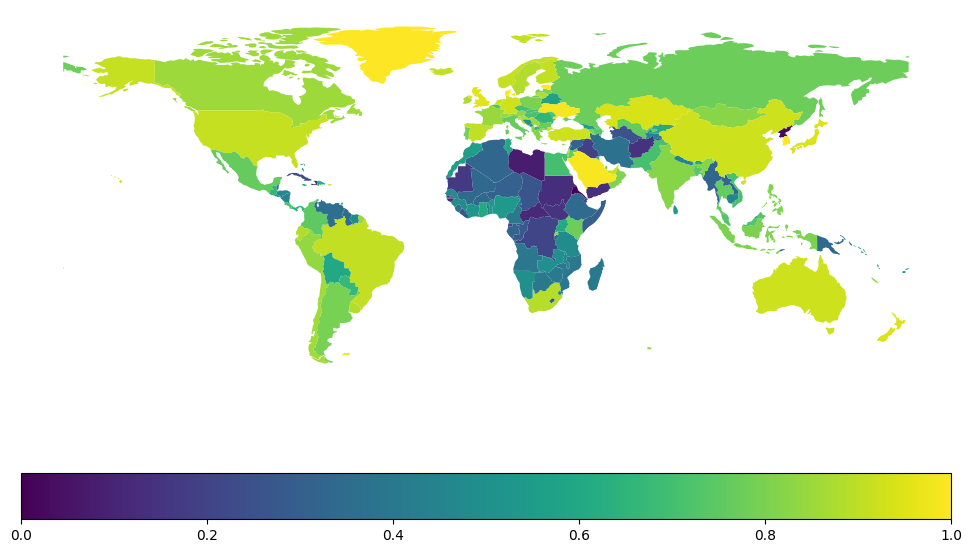
\includegraphics[width=1\linewidth]{figuras/mapa_coropletico_paises_osi}
	\label{fig:mapa_coropletico_paises_osi}
	\footnotesize{Fonte: elaboração própria baseada em \cite{ONU_EGDI_mapa}.}
\end{figure}

\begin{figure}[H]
	\centering
	\caption{TII dos países do mundo em 2024}
	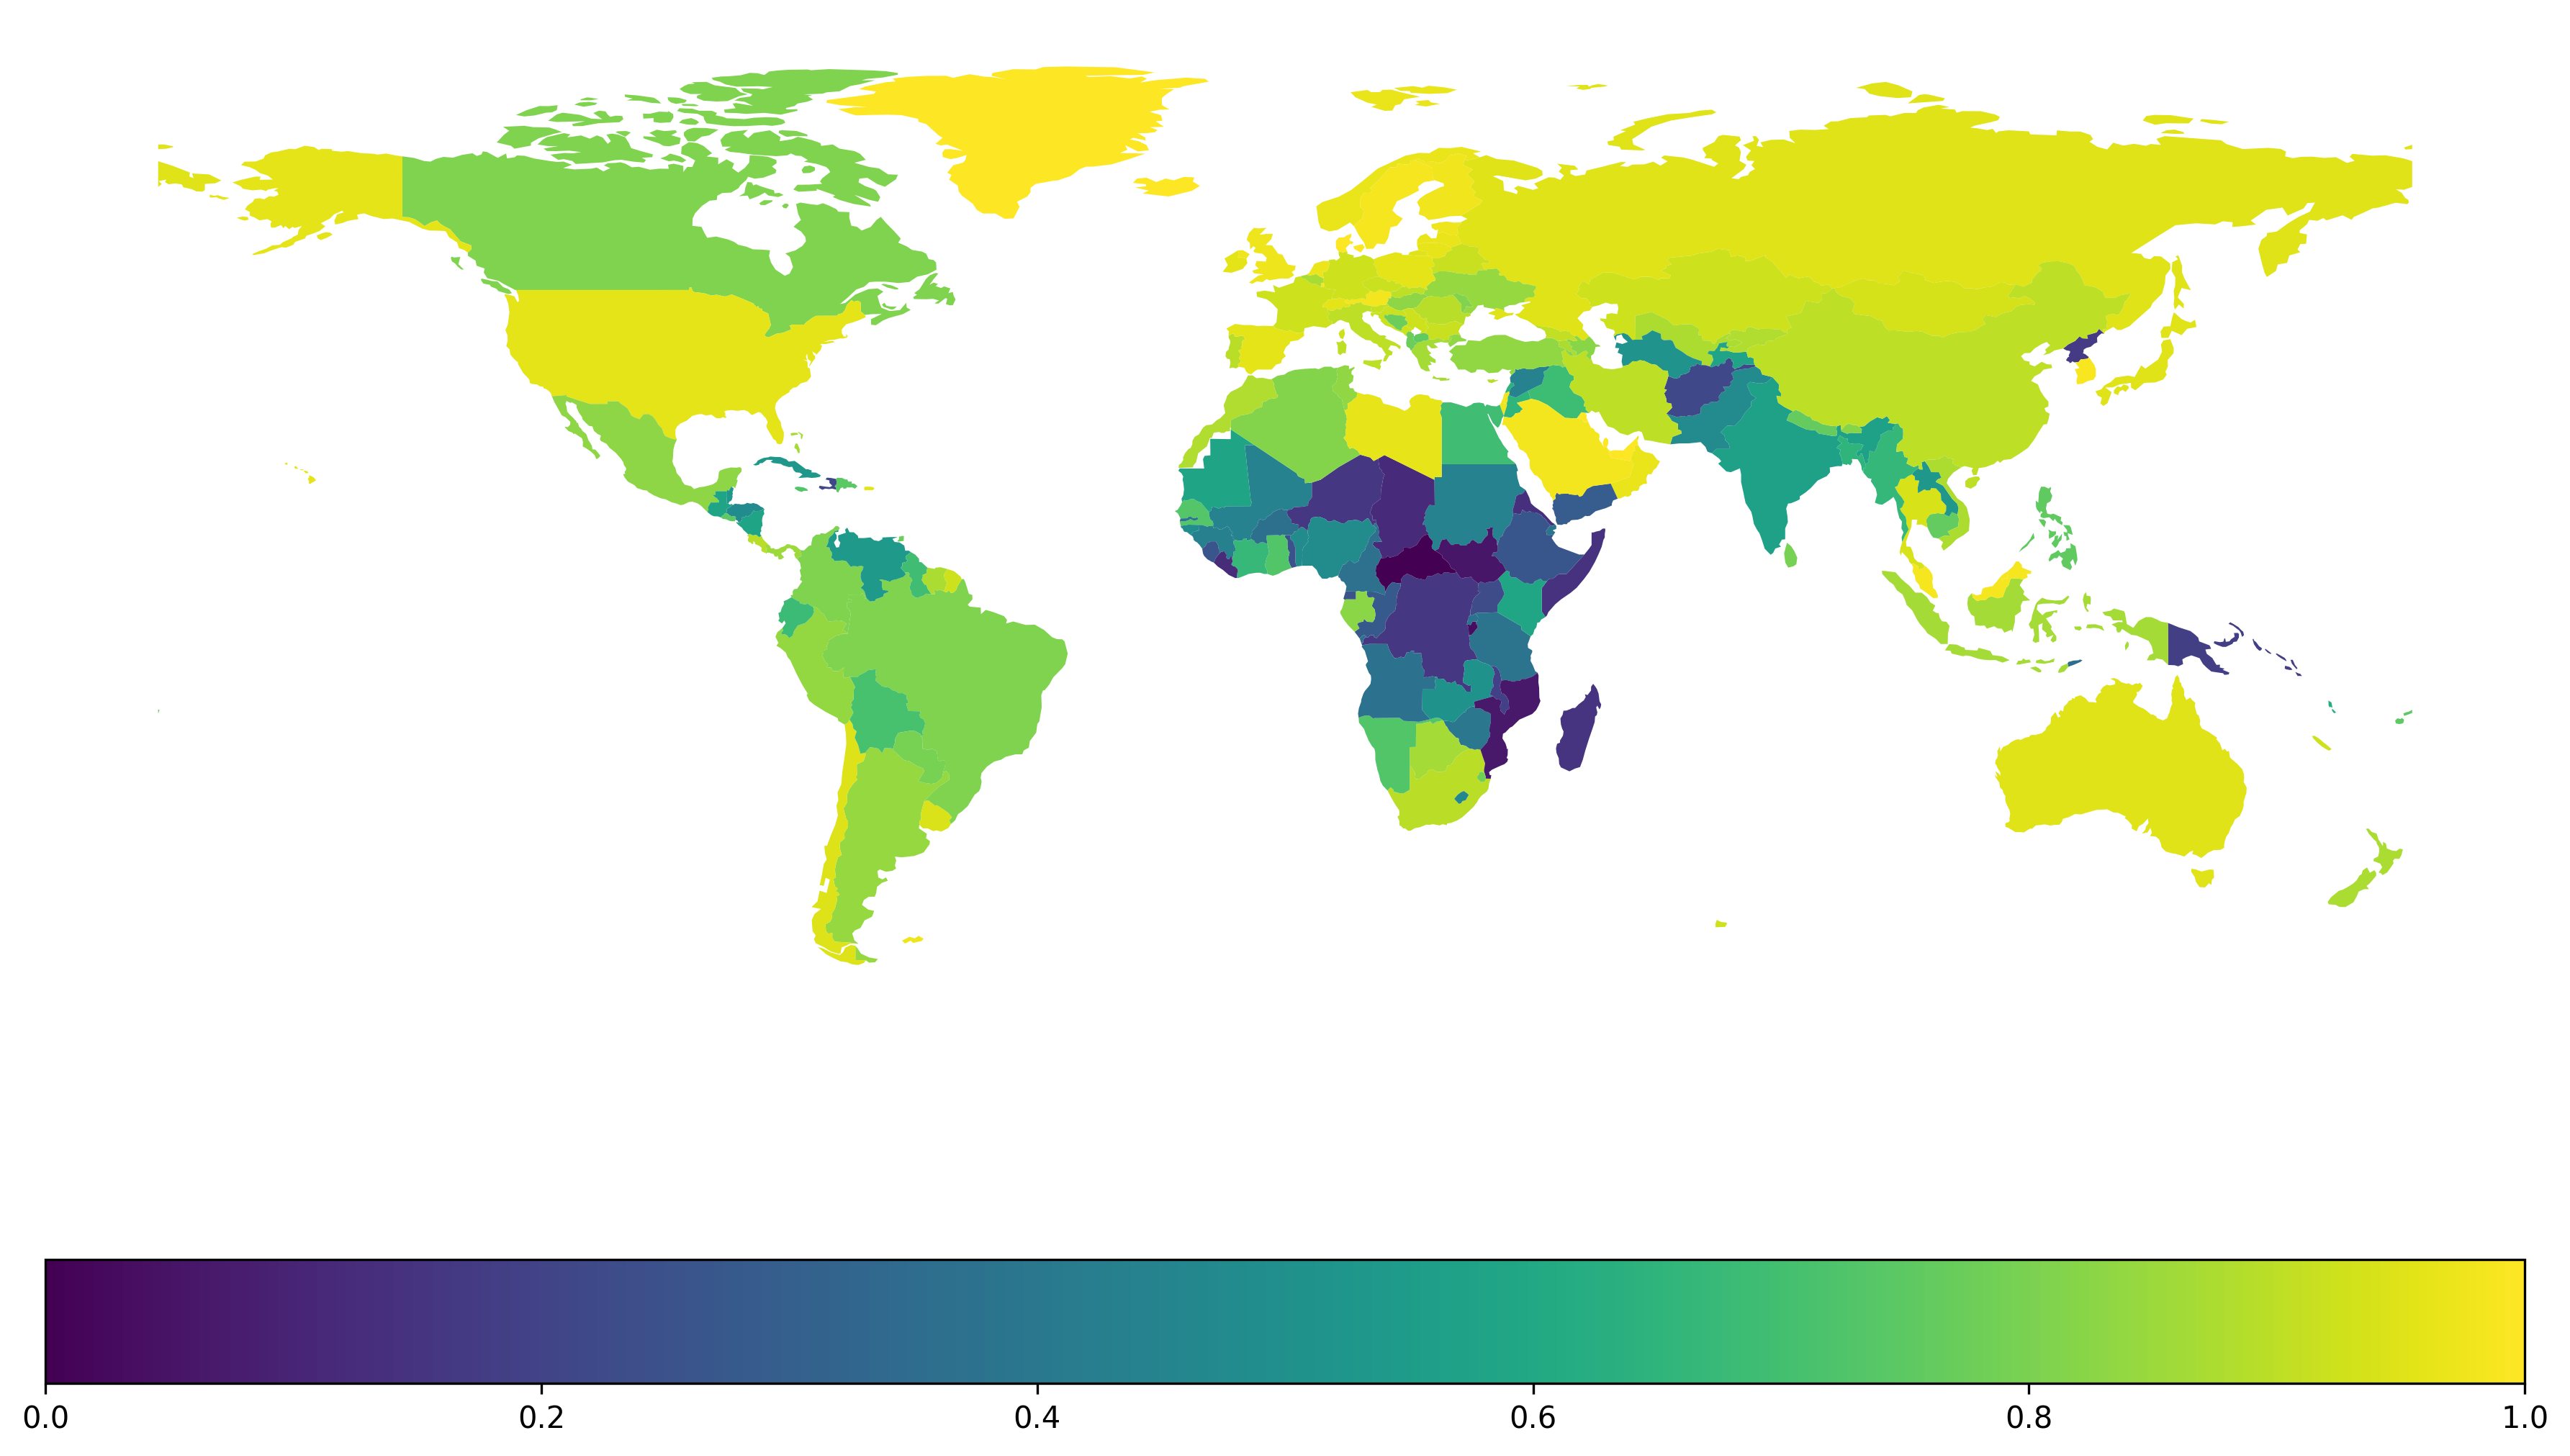
\includegraphics[width=1\linewidth]{figuras/mapa_coropletico_paises_tii}
	\label{fig:mapa_coropletico_paises_tii}
	\footnotesize{Fonte: elaboração própria baseada em \cite{ONU_EGDI_mapa}.}
\end{figure}

Conforme exposto pelas figuras \ref{mapa_coropletico_paises_egdi}, \ref{mapa_coropletico_paises_epi}, \ref{mapa_coropletico_paises_hci}, \ref{mapa_coropletico_paises_hci} e \ref{mapa_coropletico_paises_tii}, o Brasil se destaca sempre tendo pontuação em alta em qualquer indicador. Para enter a situação do Brasil, comparou-se seu EGDI, seus componentes e o EPI com a média mundial. A figura \ref{fig:comparacao_egdi_brasil_mundo} expõe os valores do EGDI, seus componentes e o EPI do Brasil e a média mundial.

\begin{figure}[H]
	\centering
	\caption{EGDI, seus componentes e o EPI do Brasil e a média mundial em 2024}
	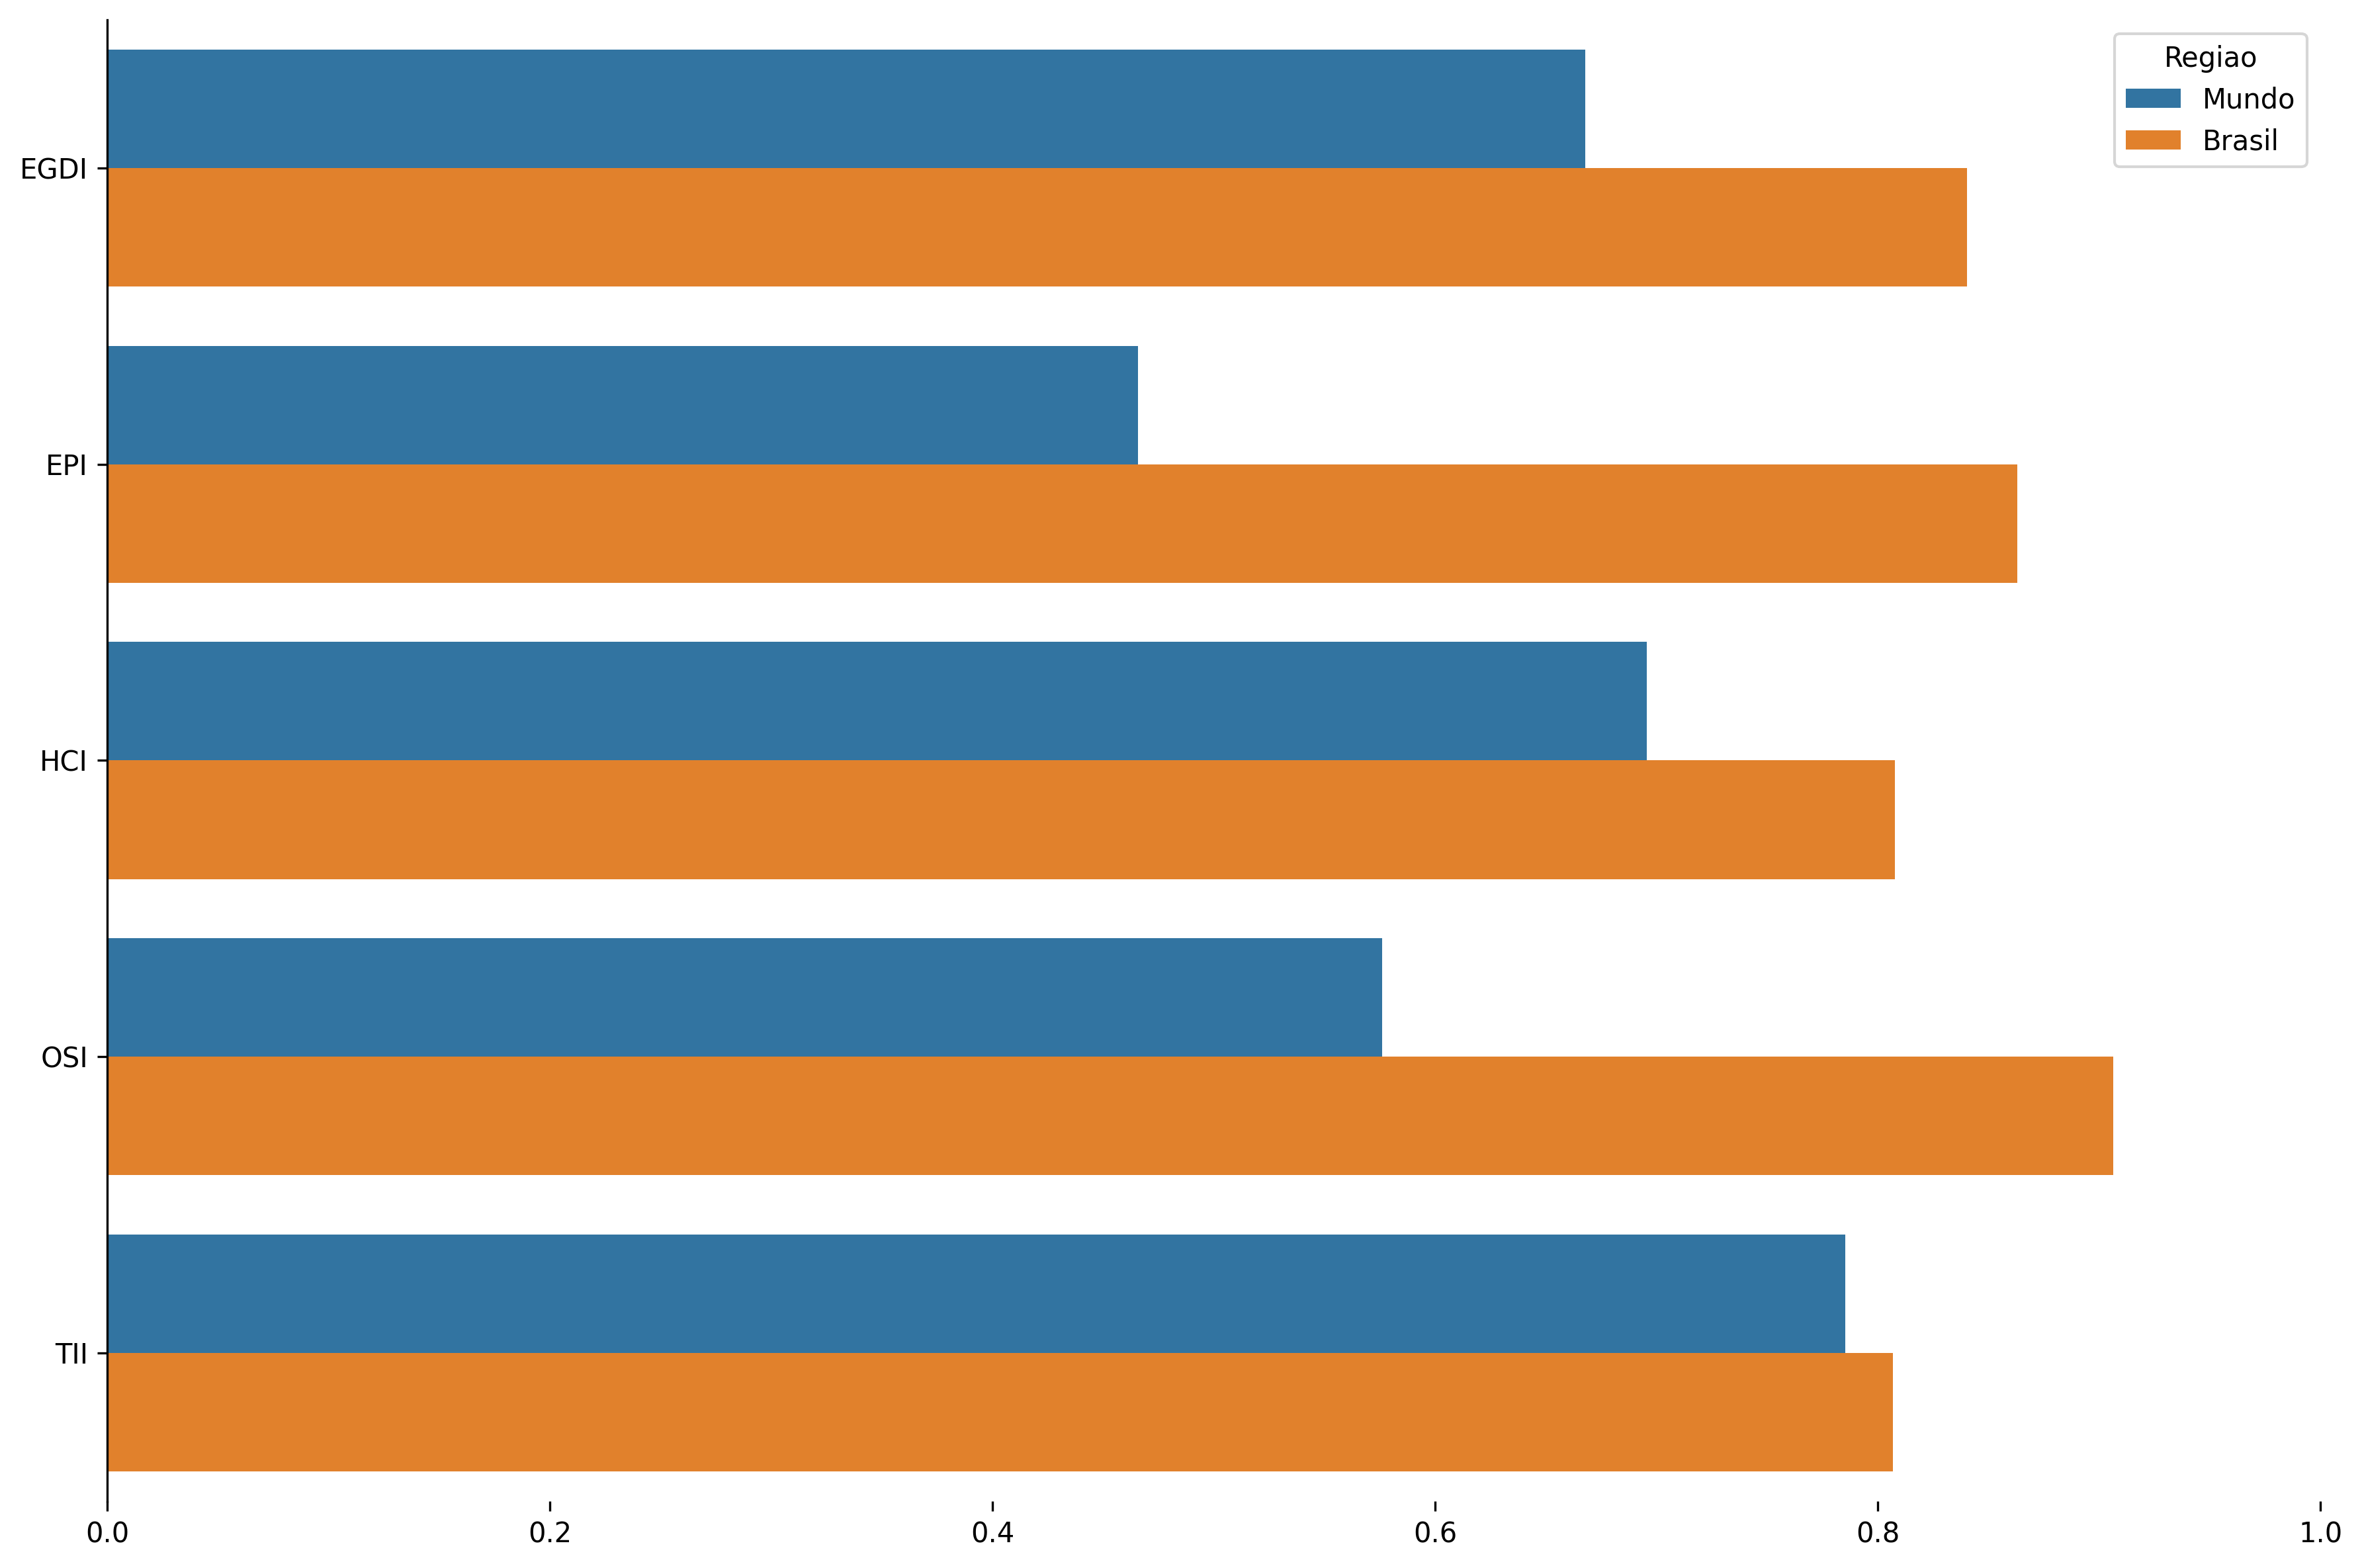
\includegraphics[width=1\linewidth]{figuras/comparacao_egdi_brasil_mundo}
	\label{fig:comparacao_egdi_brasil_mundo}
	\footnotesize{Fonte: elaboração própria baseada em \cite{ONU_EGDI_mapa}.}
\end{figure}

Da análise da figura \ref{fig:comparacao_egdi_brasil_mundo}, destaque que o Brasil está acima da média mundial em todos os índicadores. Apenas o TII mundial se aproxima do valor atingido pelo Brasil. Concomitantemente, analisou-se se o EGDI tem relação com o índice de democracia, PIB \textit{per capita} PPC em USD e com os gastos públicos como porcentagem do PIB eleitoral.

Quando o EGDI foi comparado com o índice de democracia eleitoral, descobriu-se que o coeficiente de correlação é 0,2975069. Em razão da fraca correlação entre EGDI e índice de democracia eleitoral, optou-se pelo PIB \textit{per capita} PPC em USD e pelos gastos públicos como porcentagem do PIB. Assim, objetivando descobrir se há correlação entre o PIB \textit{per capita} PPC em USD e gastos públicos como porcentagem do PIB com o EGDI, seus componentes e o EPI, foram descobertos e analisados os coeficientes de correlação resultantes dos relacionamentos citados.

O resultado foi dividido nas figuras \ref{fig:correlacao_egdi_indicedemocraciaeleitoral}, \ref{fig:correlacao_egdi_pib} e \ref{fig:correlacao_egdi_gastospublicos}.

\begin{figure}[H]
	\centering
	\caption{Coeficientes de correlação entre EGDI, seus componentes e o EPI com o índice de democracia eleitoral}
	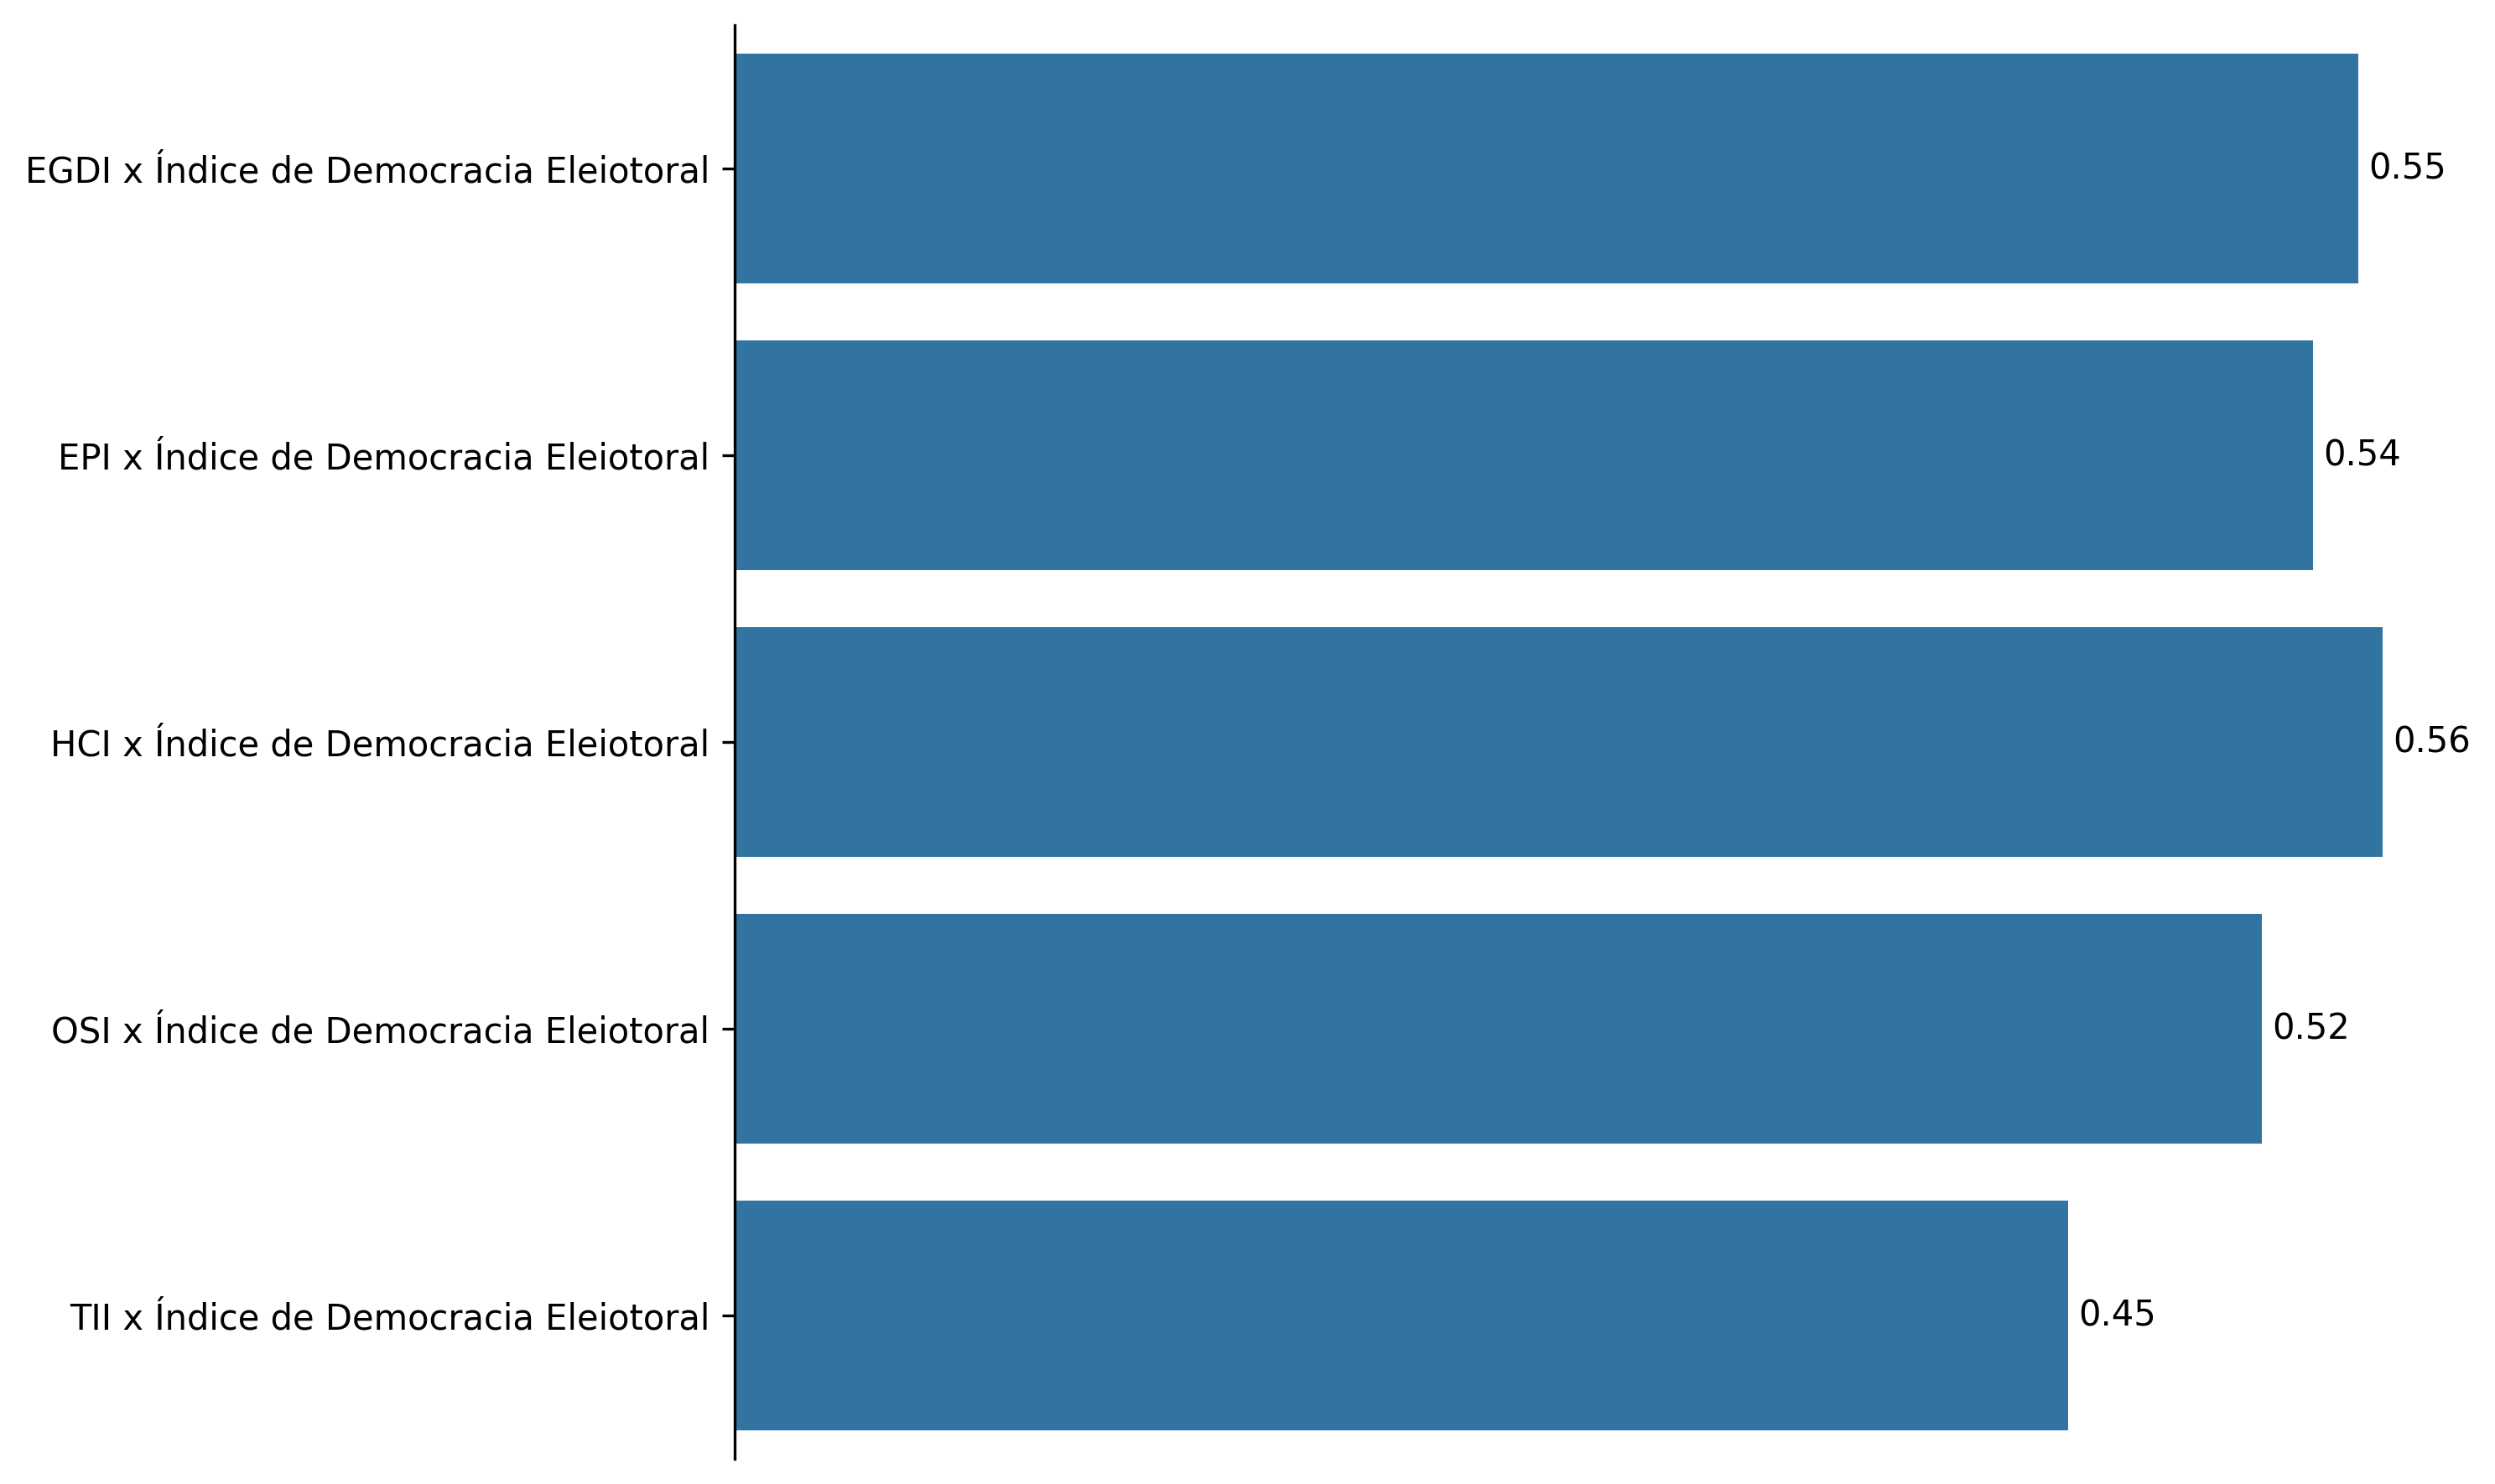
\includegraphics[width=1\linewidth]{figuras/correlacao_egdi_indicedemocraciaeleitoral.png}
	\label{fig:correlacao_egdi_indicedemocraciaeleitoral}
	\footnotesize{Fonte: elaboração própria baseada em \cite{WB_pib_per_capita_países}.}
\end{figure}

\begin{figure}[H]
	\centering
	\caption{Coeficientes de correlação entre EGDI, seus componentes e o EPI com o PIB \textit{per capita} PPC}
	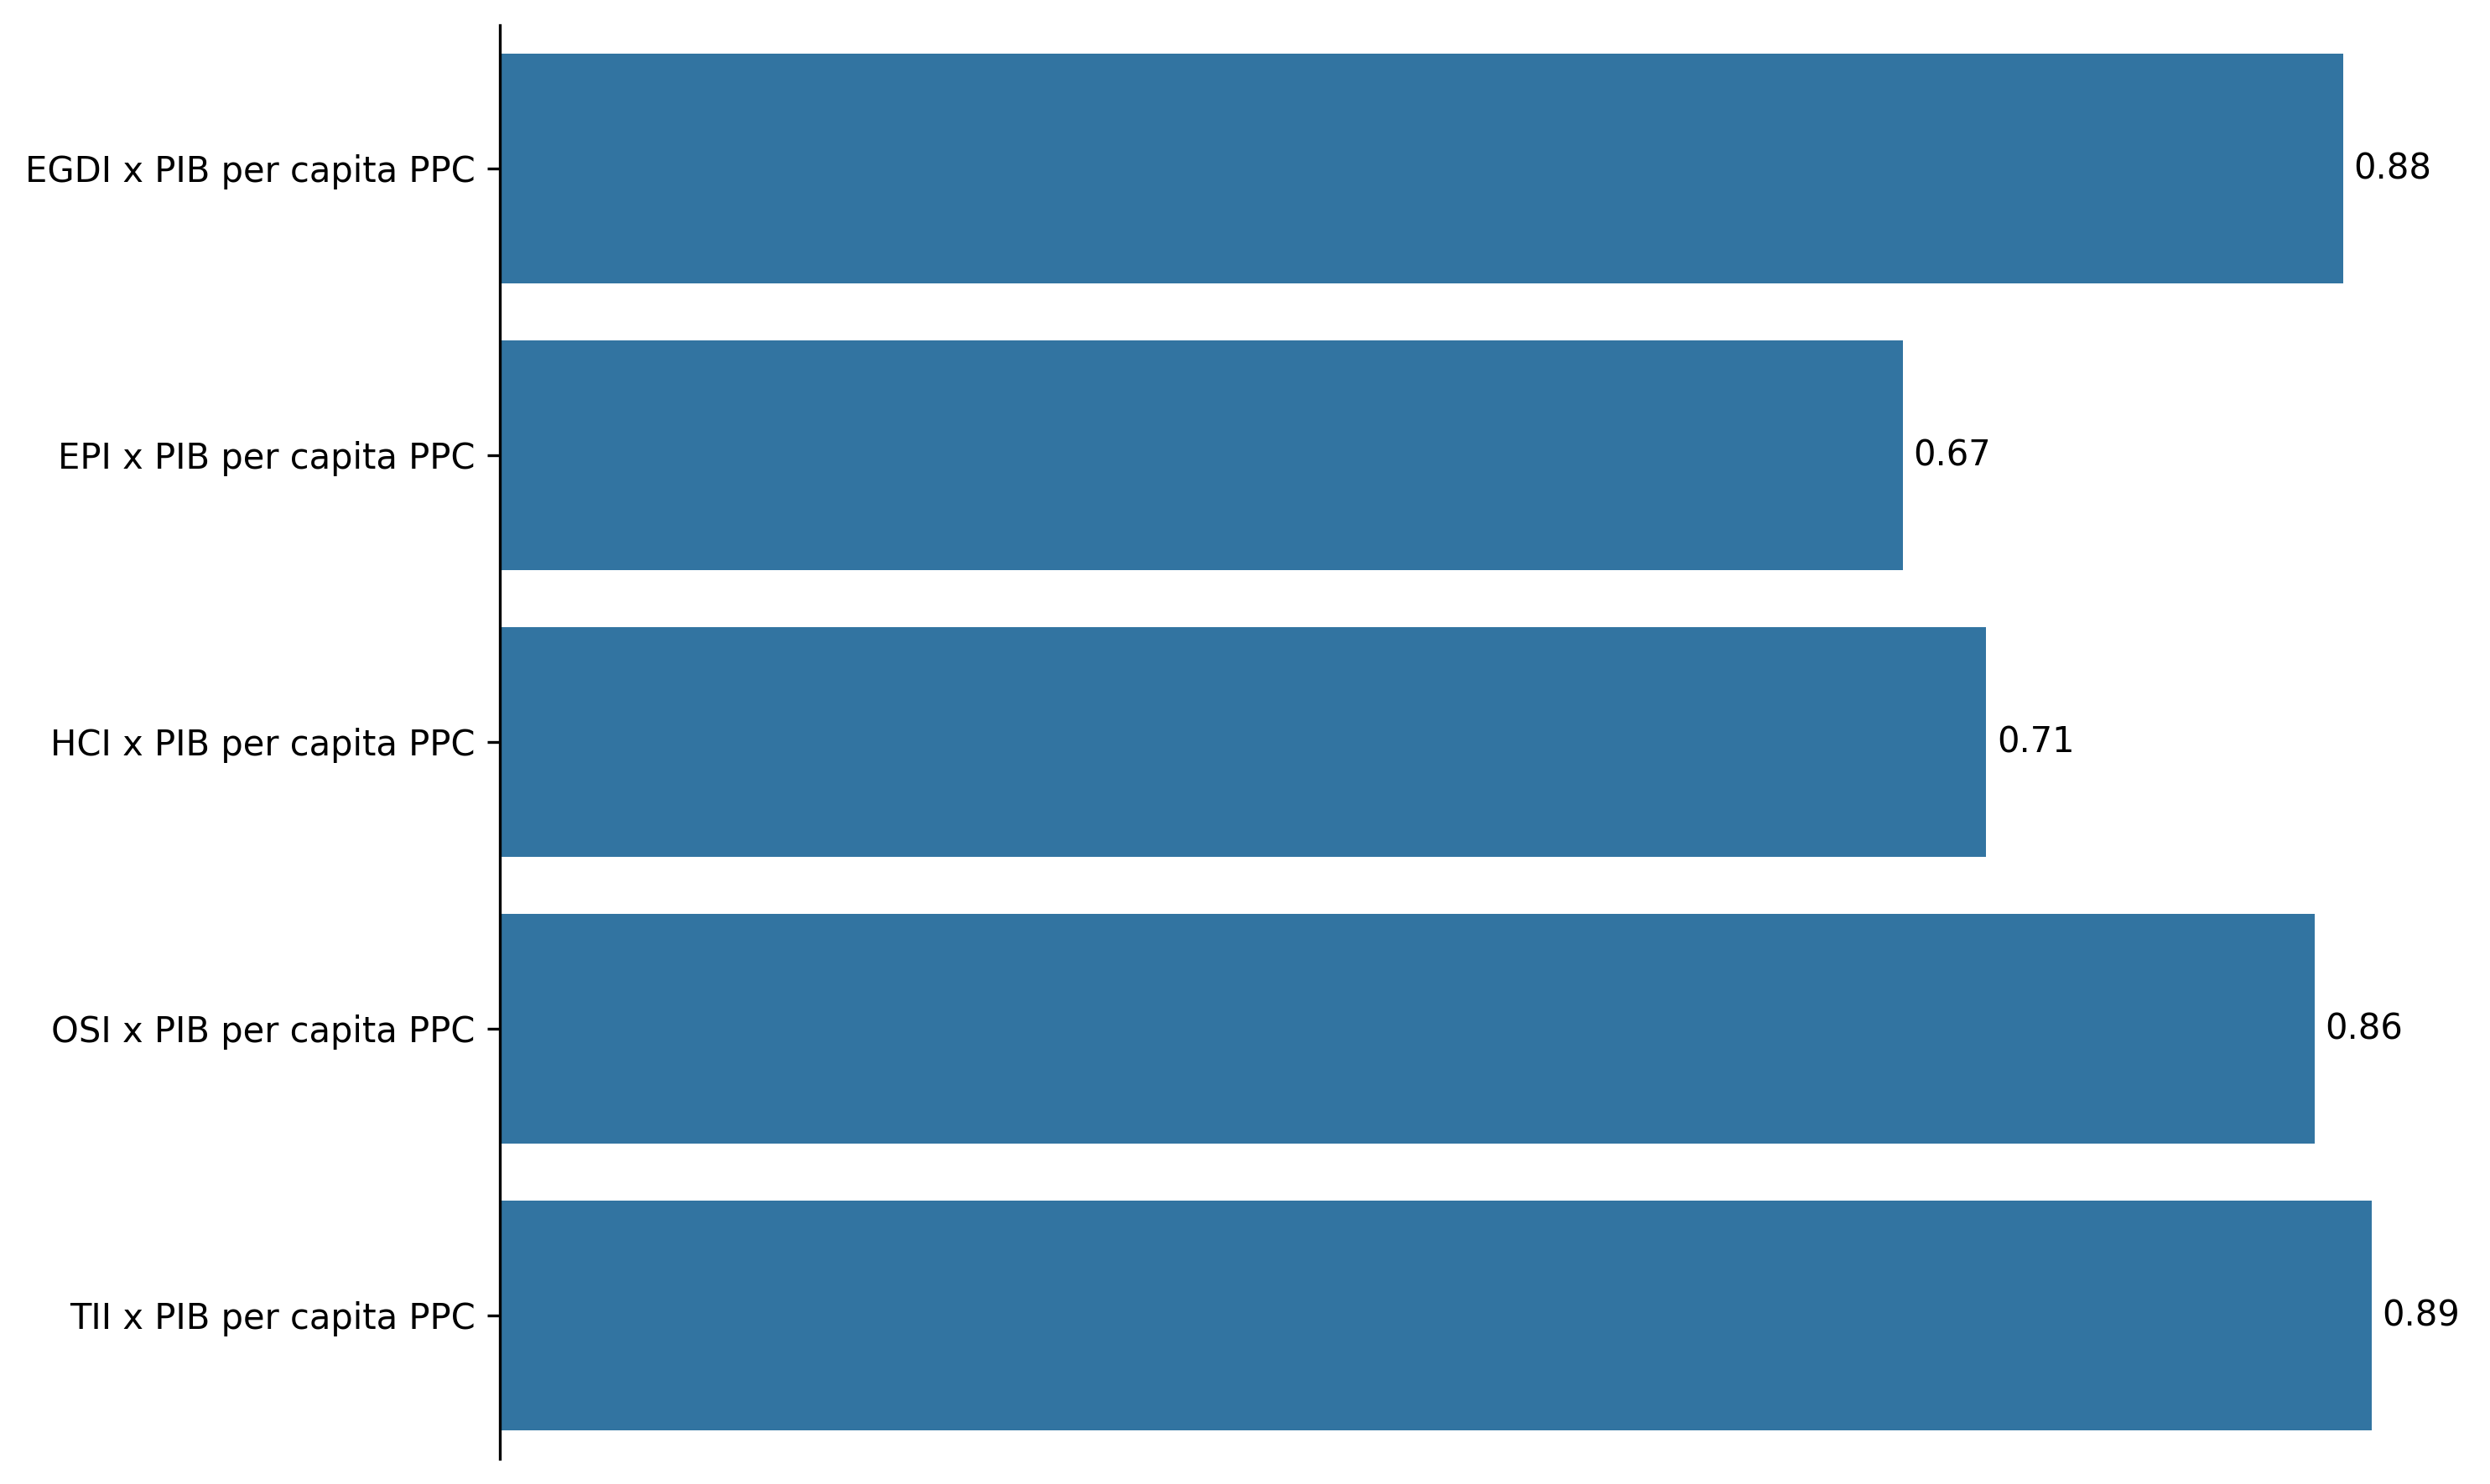
\includegraphics[width=1\linewidth]{figuras/correlacao_egdi_pibpercapitapcc.png}
	\label{fig:correlacao_egdi_pibpercapitapcc}
	\footnotesize{Fonte: elaboração própria baseada em \cite{WB_pib_per_capita_países}.}
\end{figure}

\begin{figure}[H]
	\centering
	\caption{Coeficientes de correlação entre EGDI, seus componentes e o EPI com os gastos públicos como percentual do PIB}
    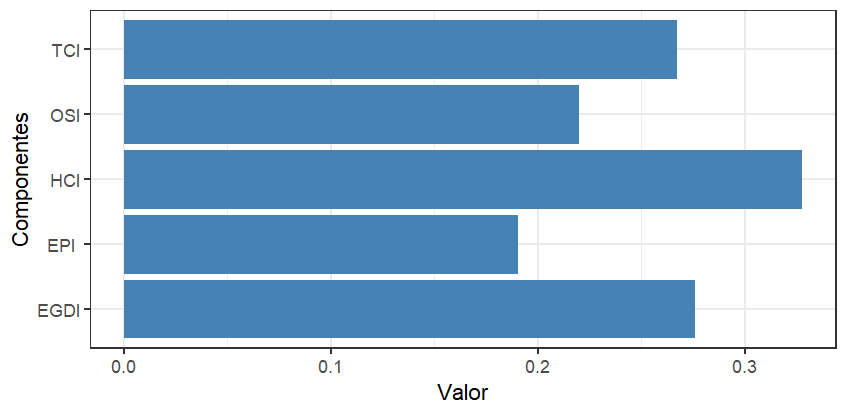
\includegraphics[width=1\linewidth]{figuras/correlacao_egdi_gastospublicos.png}
	\label{fig:correlacao_egdi_gastospublicos}
	\footnotesize{Fonte: elaboração própria baseada em \cite{FMI_gov_expenditure}.}
\end{figure}

Descobriu-se que o EGDI, seus componentes e o EPI quando comparados com o PIB \textit{per capita} PPC têm coeficientes de correlação acima de 0,6, o que indica que há correlação forte entre as variáveis. Do resultado, deduz-se que há uma tendência do crescimento do PIB de afetar positivamente o EGDI, que seguiria a tendência de crescimento.

Já a relação entre o EGDI, seus componentes e o EPI quando comparados com os gastos públicos como percentual do PIB indica uma fraca correlação, que, no máximo, passou um pouco de 0,3. Disso, extrai-se o entendimento de que as variáveis são independentes entre si.

Resumidamente, interpreta-se que quanto mais economicamente forte for um país, mais orçamento público ele tem disponível para investir em digitalização do serviço público. Contrariamente, gastos públicos como percentual do PIB não interferem no aspecto do governo eletrônico, pois demonstram que há múltiplos objetivos do poder público a serem executados na forma de gastos públicos, não exclusivamente ligados a governo eletrônico.

\cite{singh2007country}, em seu artigo de 2007, cita que uma explicação possível para o padrão de resultados observados - a baixa correlação entre a importância das tecnologias de informação e comunicação com a governança pública - indica que as novidades apresentadas pelas TIC limitam o governo eletrônico.

Complementarmente, \cite{singh2007country} argumenta que, como novas tecnologias inovadoras têm custo financeiro e conferem benefícios aos que podem ter acesso a elas. Contudo, conforme são utilizadas para implementar governo eletrônico, se tornam mais acessíveis. Como consequência, o papel mediador principal da infraestrutura de TIC pode ser enfraquecido; enquanto o capital humano e a qualidade da governança podem ganhar influência.

 Considerando o argumento de \cite{singh2007country}, ele reforça a importância de indicadores como o EGDI para a implementação de governo eletrônico, pois conforme os custos de criação e implementação de novas tecnologias são democratizados, é possível expandir a infraestrutura de TIC do governo eletrônico para focar na melhora dos demais componentes do EGDI.

Além da ideia supracitada, \cite{singh2007country} reforça a noção de que altos gastos públicos como porcentagem do PIB não impactam em um valor equivalente de EGDI.

Corroborando a análise desta seção, apresentar-se-ão ideias de 4 autores via revisão da literatuta.

Inicialmente, \cite{alisherovna2021whether} chegou a uma conclusão similar presente nesta seção, demonstrando que o EGDI impacta positivamente a taxa de crescimento do PIB dos países, conforme demonstrado na figura \ref{fig:usmanova_egdi_gdp}.

\begin{figure}[H]
	\centering
	\caption{Como os países são posicionados em torno do EGDI de acordo com sua taxa de crescimento do PIB}
	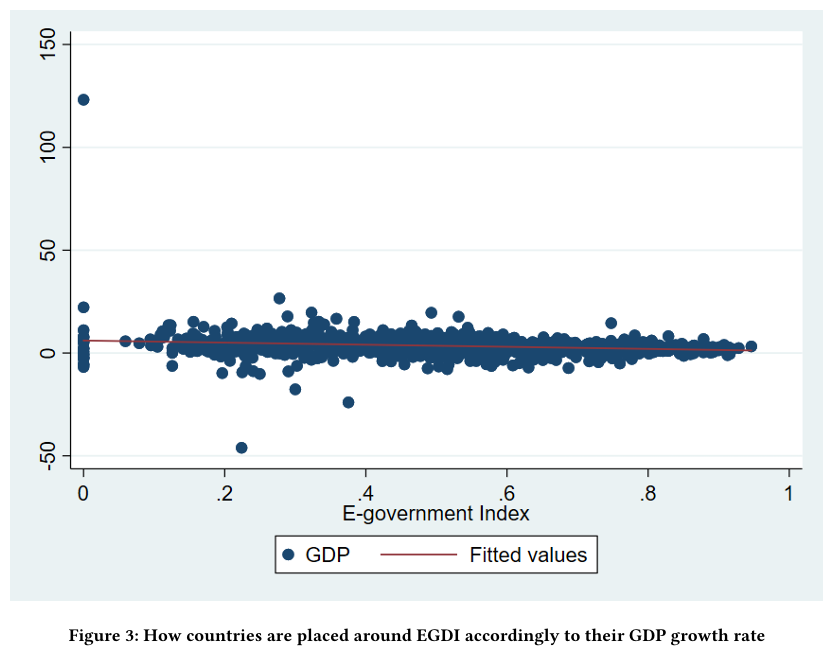
\includegraphics[width=0.8\linewidth]{figuras/usmanova_egdi_gdp}
	\label{fig:usmanova_egdi_gdp}
	\\ \footnotesize{Fonte: \cite{alisherovna2021whether}.}
\end{figure}

Da figura \ref{fig:usmanova_egdi_gdp}, nota-se como os pontos estão muito próximos da linha de tendência, o que indica forte correlação. Tal como a forte apresentada na figuras \ref{fig:correlacao_egdi_pib}, o EGDI tem influência em vários aspectos do PIB.

Em segundo lugar, \cite{kotenok2020government} argumenta que em sua pesquisa, partiu-se do princípio de que o governo eletrônico tem um impacto direto ou indireto, ou ambos, na economia; a análise de regressão em painel que utiliza o índice do PIB como variável dependente forneceu uma ideia intuitiva de que o índice desenvolvido tem um impacto potencial nos processos econômicos.

Em razão do pressuposto apresentado no parágrafo anterior, \cite{kotenok2020government} complementa que podem concluir
que o impacto do governo eletrônico pode impulsionar a inovação ou
mesmo ser um componente importante na compreensão de como a
economia é transformada devido à tecnologia.

Em terceiro lugar, \cite{kumar2020cultural} cita que seu estudo utiliza dados secundários sobre cultura nacional e desenvolvimento do governo eletrônico para explorar as relações entre as dimensões culturais e o desenvolvimento do governo eletrônico. Pode-se concluir, a partir deste estudo, que a cultura nacional influencia significativamente o desenvolvimento do governo eletrônico em um país.

\cite{kumar2020cultural} complementa que uma pesquisa das Nações Unidas indica que o desenvolvimento de um programa de governo eletrônico culturalmente relevante aproxima os cidadãos do governo. Os resultados mostraram que o aspecto de que o desenvolvimento econômico, medido pelo PIB per capita, desempenha um papel importante na indicação da preferência por serviços de governo eletrônico.

\cite{kumar2020cultural} finaliza argumentando que cultura e desenvolvimento econômico estão inter-relacionados. Portanto, os países desenvolvidos e em desenvolvimento respondem de forma diferente à recepção do governo eletrônico.

Finalmente, \cite{ziolo2022government} argumenta que a análise fornece diversas conclusões de significativa importância cognitiva e prática, especialmente do ponto de vista da compreensão dos fatores de crescimento e da definição das diretrizes da política econômica. Ao destacar a intensidade dos processos de desenvolvimento da administração eletrônica, os autores apontaram seu impacto nas esferas ambiental, social e econômica, relevantes para o crescimento sustentável.

\cite{ziolo2022government} descobriu que a correlação observada entre o nível de desenvolvimento do governo eletrônico e as áreas ambiental, social e econômica parece ser significativa. Essa correlação implica que a digitalização dos processos administrativos pode ter um impacto real no desenvolvimento sustentável,
promovendo, assim, mudanças positivas em todas as suas três esferas.

Para \cite{ziolo2022government}, o que parece extremamente importante para os processos de tomada de decisão é a relação adicional revelada entre as áreas investigadas acima em relação aos desfasamentos temporais. Em razão disso,  investir no desenvolvimento de infraestrutura digital e serviços eletrônicos governamentais traz múltiplos benefícios reais a longo prazo e tem um impacto direto em todas as três áreas relevantes para o desenvolvimento sustentável moderno.

De forma conclusiva, para \cite{ziolo2022government}, essa relação de longo prazo é particularmente relevante para identificar questões ambientais cujos efeitos parecem se manifestar claramente 10 a 15 anos após a implementação de medidas administrativas. Isso é fortemente evidente no caso da variável que representa a contribuição dos impostos ambientais para o PIB. Essa variável é considerada hoje um indicador da nossa evolução rumo à economia verde.

\section{Indicadores de TIC de governo eletrônico}
\label{indicadores_tic_egov}

A ONU tem os indicadores de TIC de governo eletrônico como algo complementar ao EGDI. Os indicadores são, conforme \cite{ONU_ICT_in_government_indicators}:

\begin{itemize}
	\item Existência de estratégia nacional de governo eletrônico ou equivalente;
	\item Existência de identidade digital para acessar ou outra forma de autenticação requirida para poder acessar serviços online;
	\item Existência de um portal de compras governamentais.
\end{itemize}

Os resultados globais dos indicadores estão presentes nas figuras \ref{fig:national_government_strategy}, \ref{fig:national_identity} e \ref{fig:procurement_portal}.

\begin{figure}[H]
	\centering
	\caption{Indicador de TIC de governo eletrônico: Existência de estratégia nacional de governo eletrônico ou equivalente}
	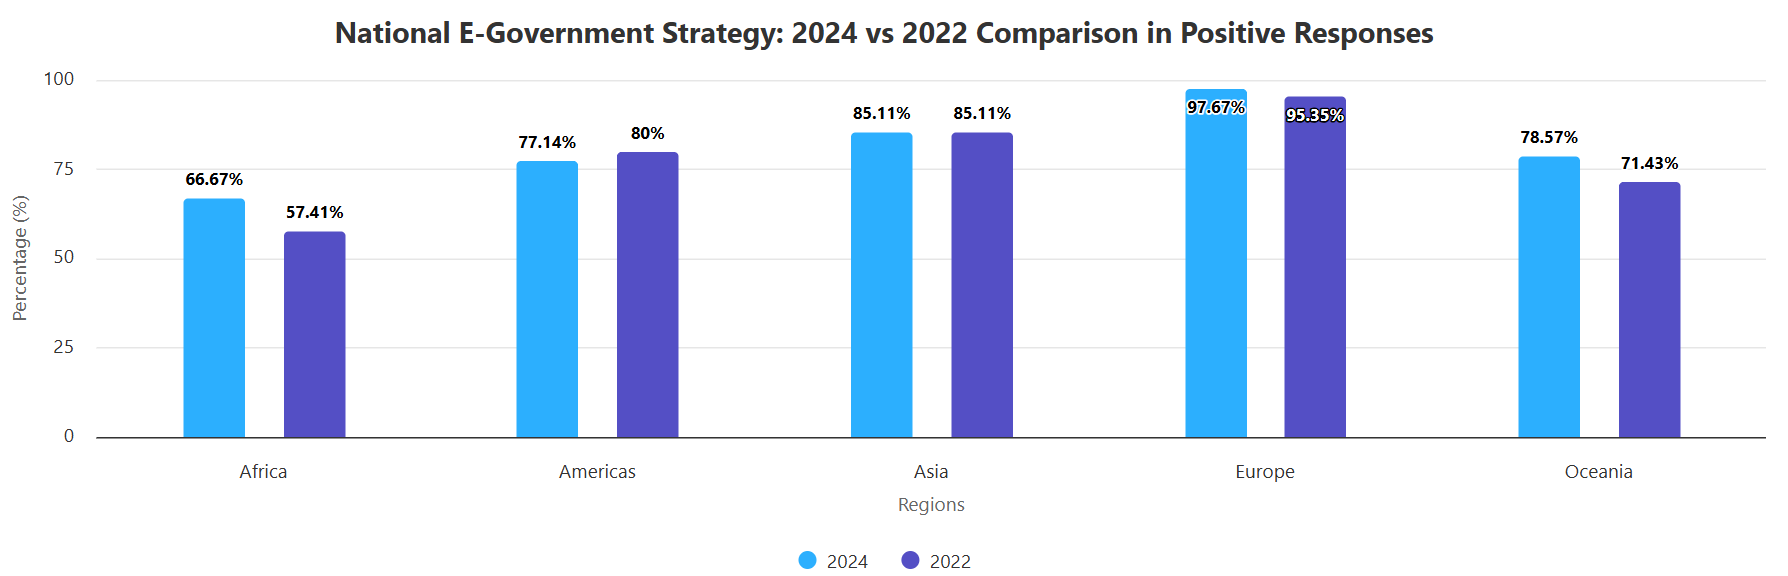
\includegraphics[width=1\linewidth]{figuras/national_government_strategy}
	\label{fig:national_government_strategy}
	\footnotesize{Fonte: \cite{ONU_ICT_in_government_indicators}.}
\end{figure}

\begin{figure}[H]
	\centering
	\caption{Indicador de TIC de governo eletrônico: Existência de identidade digital para acessar ou outra forma de autenticação requirida para poder acessar serviços online}
	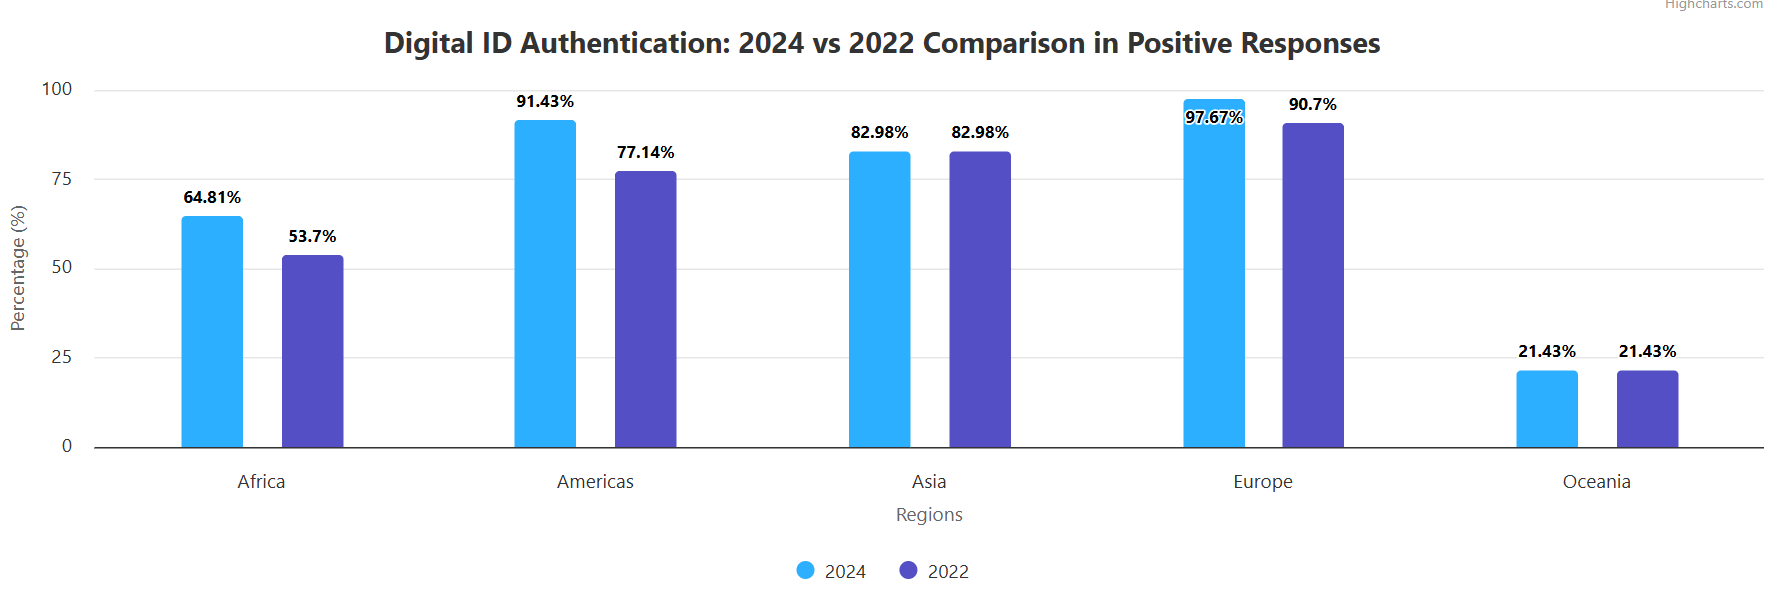
\includegraphics[width=1\linewidth]{figuras/digital_identity}
	\label{fig:national_identity}
	\footnotesize{Fonte: \cite{ONU_ICT_in_government_indicators}.}
\end{figure}

\begin{figure}[H]
	\centering
	\caption{Indicador de TIC de governo eletrônico: Existência de um portal de compras governamentais}
	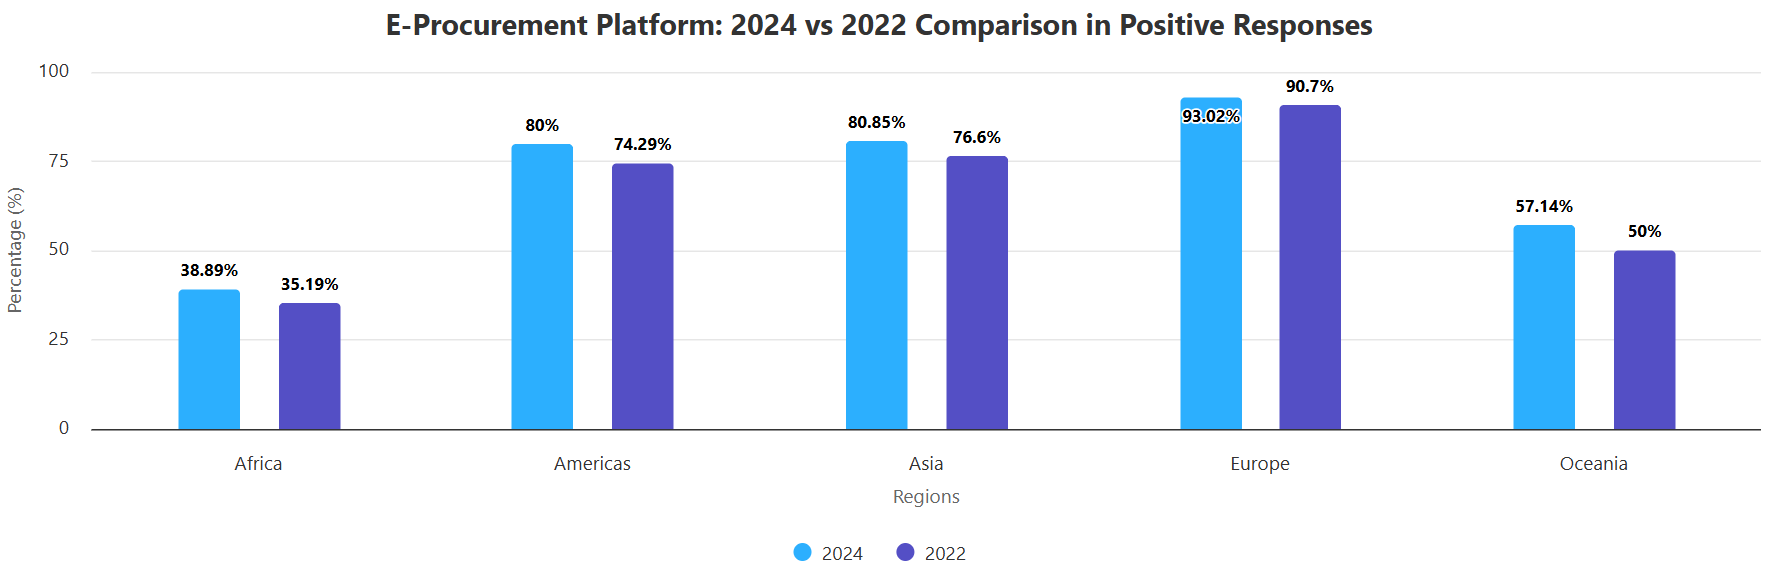
\includegraphics[width=1\linewidth]{figuras/procurement_portal}
	\label{fig:procurement_portal}
	\footnotesize{Fonte: \cite{ONU_ICT_in_government_indicators}.}
\end{figure}

Extraí-se das três figuras que a Europa foi o continente cujos mais respondem que têm seguido os indicadores, superando os 90\%. A Oceania foi o continente que menos implementou políticas de identidade digital para acesso a serviços online. África e Oceania tiveram um desempenho ruim na implementação de portais de compra governamentais. O continente americano apresentou bom desempenho nos três indicadores.

Como consequência da análise dos resultados presentes nas figuras \ref{fig:national_government_strategy}, \ref{fig:national_identity} e \ref{fig:procurement_portal}, buscou-se entender a seguinte situação registrada nos 2022 e 2024, anos em que os indicadores foram medidos: qual é a porcentagem de países que responderam nenhuma, uma, duas ou todas as perguntas. Elas usam sim ou não para confirmar a aplicação dos indicadores no país.

A resposta ao questionamento está presente na figura \ref{fig:ticegov_soma_respostas_positivas}.

\begin{figure}[H]
	\centering
	\caption{Respostas positivas aos indicadores de TIC de governo eletrônico de 2024}
	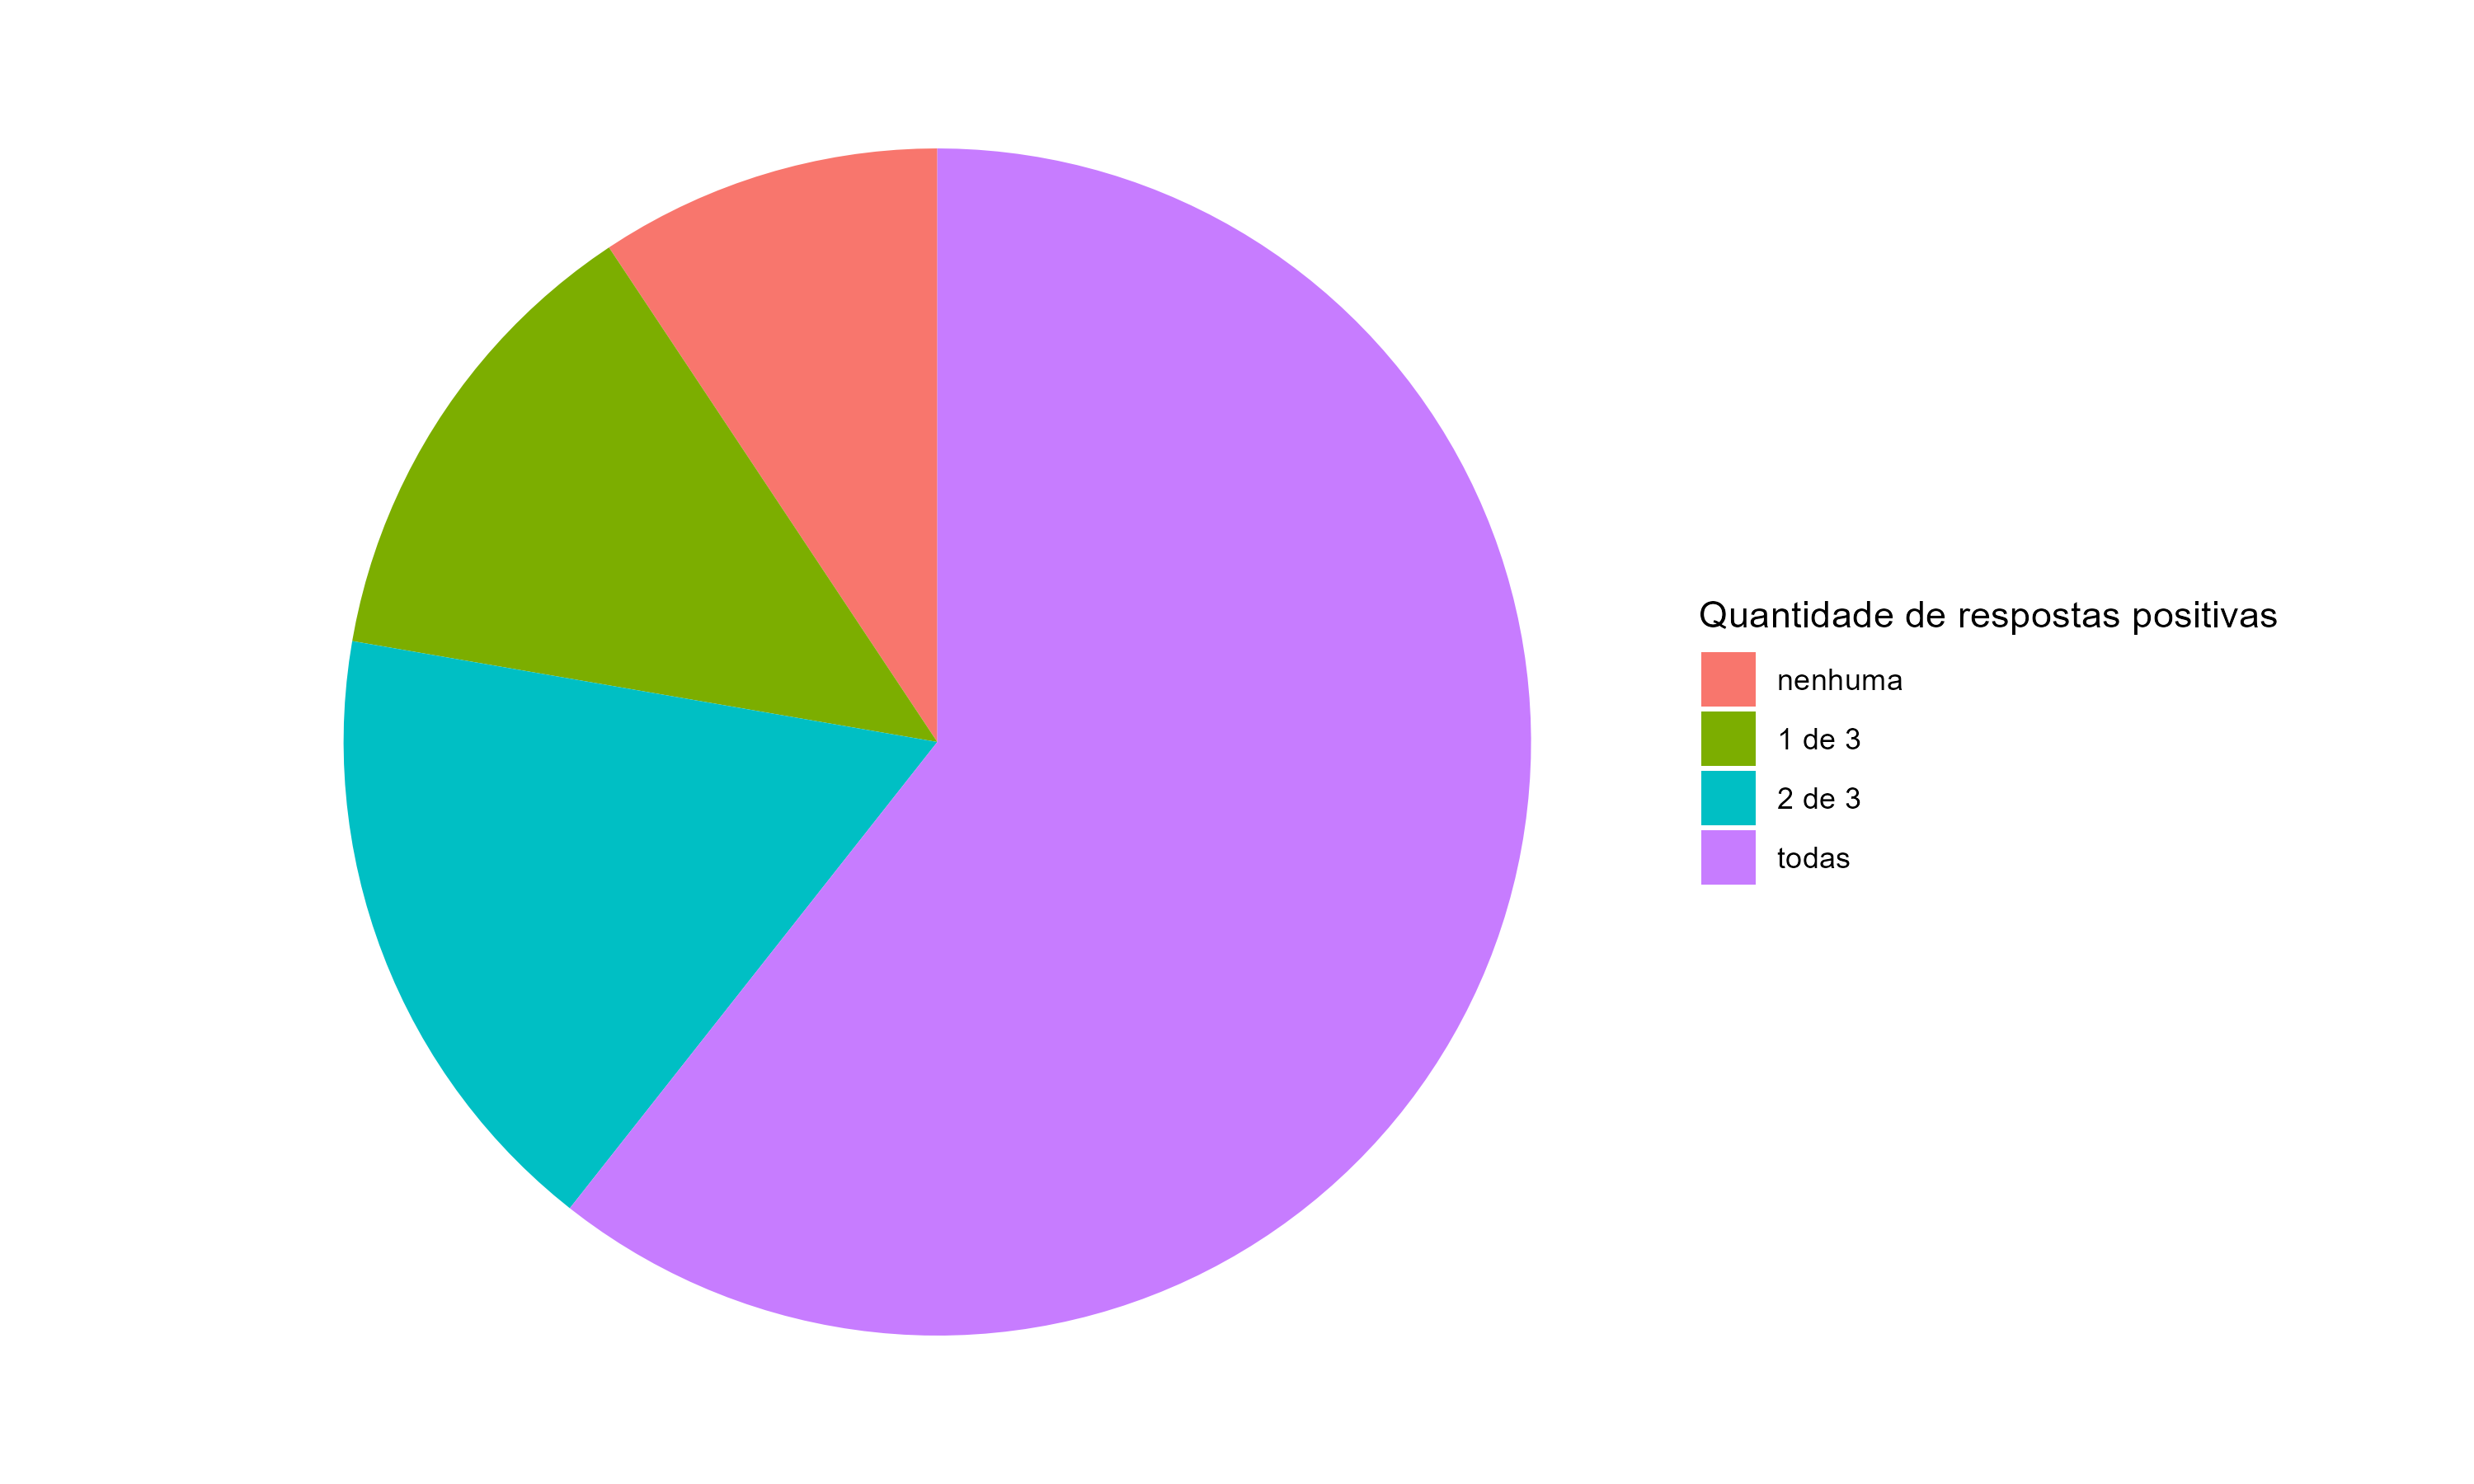
\includegraphics[width=1\linewidth]{figuras/ticegov_soma_respostas_positivas}
	\label{fig:ticegov_soma_respostas_positivas}
	\footnotesize{Fonte: \cite{ONU_ICT_in_government_indicators}.}
\end{figure}

Em 2024, mais da metade dos países respondeu positivamente às três perguntas. O Brasil faz parte desse grupo. Tal resultado indica que mais da metade dos países está investindo em TIC de governo eletrônico em seus territórios.

O resultado apresentado anteriormente demonstra como o compromisso do Brasil com sua política pública de implementação, manutenção e a evolução do seu governo eletrônico.

No tocante ao indicador \textbf{existência de estratégia nacional de governo
eletrônico ou equivalente}, \cite{brasil_engd} cita que a ENGD está prevista na \href{https://www.planalto.gov.br/ccivil_03/_ato2019-2022/2021/lei/l14129.htm}{Lei do Governo Digital}. A ENGD foi formalizada pelo \href{https://www.planalto.gov.br/ccivil_03/_ato2023-2026/2024/decreto/D12069.htm}{Decreto nº 12.069, de 2024}. E é complementada pela \href{https://www.in.gov.br/en/web/dou/-/portaria-sgd/mgi-n-4.248-de-26-de-junho-de-2024-568659997}{Portaria SGD/MGI nº 4.248, de 2024}, que estabeleceu recomendações para o alcance dos objetivos da ENGD para o período de 2024 a 2027.

No tocante ao indicador \textbf{existência de identidade digital para acessar
ou outra forma de autenticação requirida para poder acessar serviços online}, ele foi alcançado no Brasil pela implementação da plataforma \textbf{GOV.BR}. 

A plataforma foi criada pelo \href{https://www.planalto.gov.br/ccivil_03/_ato2019-2022/2019/decreto/d9756.htm}{Decreto nº 9.765, de 2019}. A criação do \textbf{GOV.BR} implicou na criação do portal único do Governo Federal, sendo vedada a criação, de acordo com \cite{d9756}, a partir de 1º de julho de 2019, o registro de novos domínios “.gov.br” na internet e de aplicativos móveis em lojas de aplicativos pelos órgãos e pelas entidades da administração pública federal.

Complementarmente, \cite{d9756} obrigou, a partir de 1º de julho de 2019, a utilização do domínio raiz “gov.br”, acrescido de “/” e seguido do detalhamento do endereço, nos novos endereços de sítios eletrônicos do Governo federal.

Para \cite{mitkiewicz2024transformacao}, o Brasil possui uma trajetória de mais de duas décadas de planejamento e adoção de medidas estruturantes em diversas dimensões voltadas à implementação de uma visão de governo eletrônico/digital, abrangendo sete gestões presidenciais diferentes nesse período, sendo uma política pública de Estado.

O \textbf{GOV.BR} como canal de acesso único aos serviços públicos digitais é parte da iniciativa de Governo Digital apresentada no art. 3º, II da Lei 14.129, de 2021 - \textbf{Lei do Governo Digital}, conforme dispõe \cite{l14129}, \textit{ipsis litteris}: "Art. 3º  São princípios e diretrizes do Governo Digital e da eficiência pública: [...] II - a disponibilização em plataforma única do acesso às informações e aos serviços públicos, observadas as restrições legalmente previstas e sem prejuízo, quando indispensável, da prestação de caráter presencial;".

A Lei do Governo Digital também enquadra o \textbf{GOV.BR} dentro do conceito de \textbf{Governo como Plataforma} (art. 3º, XXIII), definido por \cite{l14129} como infraestrutura tecnológica que facilite o uso de dados de acesso público e promova a interação entre diversos agentes, de forma segura, eficiente e responsável, para estímulo à inovação, à exploração de atividade econômica e à prestação de serviços à população.

Como consequência, \cite{l14129} posiciona \textbf{Governo como Plataforma}, como: "XXIII - a implantação do governo como plataforma e a promoção do uso de dados, preferencialmente anonimizados, por pessoas físicas e jurídicas de diferentes setores da sociedade, resguardado o disposto nos arts. 7º e 11 da Lei nº 13.709, de 14 de agosto de 2018 (Lei Geral de Proteção de Dados Pessoais), com vistas, especialmente, à formulação de políticas públicas, de pesquisas científicas, de geração de negócios e de controle social;".

Outro aspecto fundamental do \textbf{GOV.BR} são as plataformas de governo digital, definidas por \cite{l14129} como ferramentas digitais e serviços comuns aos órgãos, normalmente ofertados de forma centralizada e compartilhada, necessários para a oferta digital de serviços e de políticas públicas. 

As plataformas de governo digital tem a seguinte estrutura, conforme \cite{l14129}, são instrumentos necessários para a oferta e a prestação digital dos serviços públicos de cada ente federativo, deverão ter pelo menos as seguintes funcionalidades: 

\begin{itemize}
    \item Ferramenta digital de solicitação de atendimento e de acompanhamento da entrega dos serviços públicos.
    \item Painel de monitoramento do desempenho dos serviços públicos.
\end{itemize}

O painel de monitoramento é regido pelo artigo 22 da \textbf{Lei do Governo Digital}, nos termos de \cite{l14129}, sendo o painel de monitoramento do desempenho dos serviços públicos de que trata o inciso II do caput do art. 20 deverá conter, no mínimo, as seguintes informações, para cada serviço público ofertado:

\begin{itemize}
    \item Quantidade de solicitações em andamento e concluídas anualmente.
    \item Tempo médio de atendimento.
    \item Grau de satisfação dos usuários.
\end{itemize}

Para confirmar a ideia expressa por \cite{mitkiewicz2024transformacao} de que o Brasil tem políticas públicas de Estado de governo eletrônico e digital, \cite{painel_completo_monitoramento_govbr} apresenta os resultados (até 09/08/2025) do \textbf{GOV.BR}.

\begin{figure}[H]
    \centering
    \caption{Painel Detalhado do GOV.BR}
    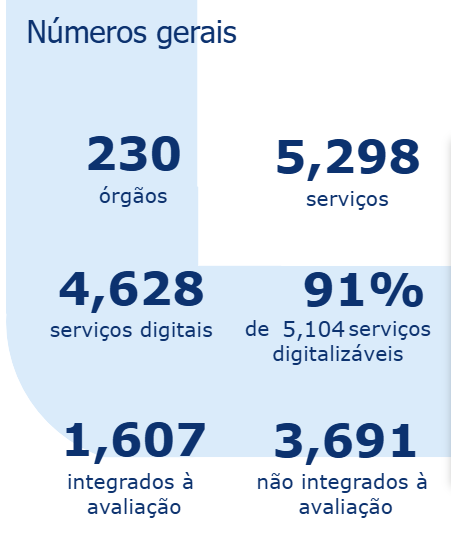
\includegraphics[width=0.5\linewidth]{figuras/painel_govbr.PNG}
    \label{fig:placeholder}
    \\ \footnotesize{Fonte: \cite{painel_completo_monitoramento_govbr},}
\end{figure}

Com mais de 90\% dos serviços públicos digitalizados, comprova-se o motivo do EGDI do Brasil ser superior à média mundial.

Finalmente, o último indicador de TIC de governo eletrônico - \textbf{existência de um portal de compras governamentais} foi implementado pela Lei nº 14.133, de 2021 - \textbf{Lei de Licitações e Contratos Administrativos}. A norma infraconstitucional, em concordância com \cite{l14133}, criou em seu ao PNCP, visando à divulgação centralizada e obrigatória dos atos exigidos pela lei e a realização facultativa das contratações pelos órgãos e entidades dos Poderes Executivo, Legislativo e Judiciário de todos os entes federativos.

\cite{l14133} expõe como condição indispensável para a eficácia do contrato e de seus aditamentos a divulgação no PNCP, contados da data da assinatura, 20 dias úteis para licitações e 10 dias úteis para contratação direta.

De forma conclusiva, \cite{l14133} argumenta que os órgãos e entidades da Administração Pública deverão utilizar o sistema de registro cadastral unificado disponível no PNCP, para efeito de cadastro unificado de licitantes, na forma disposta em regulamento.

\chapter{Digitalização do Poder Público Brasileiro}

"Este capítulo mergulha no processo de digitalização do setor público brasileiro, analisando a evolução das políticas e o impacto da tecnologia na relação entre o Estado e o cidadão. Inicialmente, exploramos o conceito de governo eletrônico, compreendido como a base tecnológica que otimiza a gestão e a oferta de serviços. Em seguida, foi detalhado seus benefícios e, de forma crítica, foi examinado as limitações que levaram à necessidade de uma abordagem mais abrangente: o governo digital.

\section{Contextualização do governo eletrônico}

\cite{tavares2022governo} afirma que as políticas públicas são a forma como se resolve os problemas da sociedade e o controle social é a forma como o cidadão interage, fiscaliza e questiona as soluções definidas para esses problemas. 

\cite{rover2009introduccao} argumenta que a interação entre as novas tecnologias, a sociedade e o Poder Público emoldura um momento único do qual emergem, simultaneamente, desafios enormes e vantagens sociais incríveis. Neste contexto, o aparecimento do governo eletrônico é uma decorrência das velhas e novas demandas da sociedade.

Para \cite{rover2009introduccao}, governo eletrônico é uma infra-estrutura única de comunicação compartilhada por diferentes órgãos públicos a partir da qual a TIC é usada de forma intensiva para melhorar a gestão pública e o atendimento ao cidadão.

Adicionalmente, como é entendido por \cite{rover2009introduccao}, o objetivo do governo eletrônico é colocar o governo ao alcance de todos, ampliando a transparências das suas ações e incrementando a participação cidadã, almejando a universalização de serviços.

\cite{singh2007country} projeta que a maturidade do governo eletrôncio pode ser considerada razoavelmente dependente de como está o estado da infraestrutura de TIC, em razão da sua capacidade de limitar o acesso aos serviços públicos digitais. 

Para \cite{singh2007country}, países com PIB per capita altos estão em melhor posição de dispor de infraestruturas difundidas, alta qualidade e físicas de TIC. Com altos níveis de acesso às TIC, os cidadãos tem uma tendência maior de usar serviços públicos digitais.

Quando os cidadãos passam a adotar os serviços públicos digitais, segundo \cite{singh2007country}, facilita ao poder público a transação completa dos serviços públicos presenciais para os digitais. A referida mudança pode ajudar na economia de recursos públicos, definindo um círculo virtuoso que justifica os investimentos em governo eletrônico.

\section{Benefícios do governo eletrônico}

Diversos autores destacam o impacto positivo do governo eletrônico na sociedade.  \cite{martins2018war} cita que os resultados encontrados indicam claramente que níveis mais altos de governo eletrônico estão associados a melhores resultados no combate à corrupção. Para \cite{kotenok2020government}, o impacto do governo eletrônico pode impulsionar a inovação ou até mesmo ser um componente importante para entender como a economia é transformada   devido à tecnologia.

\cite{martins2022digital} um nível alto de governo eletrônico podem facilitar negócios pela   diminuição do fardo das regulações em diversas áreas de negócio. \cite{sugiarti2024effect} sua pesquisa examinou a relação entre governo eletrônico e corrupção nos   estados dos Estados Unidos encontraram que o governo eletrônico aumentou   tanto as condenações por corrupção, quanto a percepção de corrupção.

Para \cite{ziolo2022government}, na União Europeia (até 2020) observou-se a correlação observada entre o nível de desenvolvimento do governo eletrônico e as áreas ambiental, social e econômica parece ser de grande importância, pois implica que a digitalização dos processos administrativos pode ter um impacto real no desenvolvimento   sustentável, promovendo, assim, mudanças positivas em todas as suas três esferas.

\section{Foco do governo eletrônico}

Contudo, para \cite{de2020governo} o foco das políticas de governo eletrônico, em geral, permanece o mesmo: aprimorar processos internos de  trabalho, sem alterações significativas na cultura e na lógica burocráticas sobre as quais se estruturam as relações que se estabelecem entre a administração pública e os cidadãos.

Assim, para \cite{cristovam2020governo} a Administração Pública brasileira tem usado as TIC no incremento de suas rotinas burocráticas. Há, ainda, o crescente uso dessas tecnologias na promoção do acesso à informação aos cidadãos. Mas ambos são usos na esteira do dito Governo eletrônico.

Consequentemente, conforme \cite{cristovam2020governo}, para se distanciar do governo eletrônico e poder implementar o governo digital, pois não se deve almeja somente o emprego incremental de TICs e a viabilização do acesso à informação, mas vai além, corporificando direitos sociais por intermédio do espaço digital.

Nesse sentido, quando \cite{cristovam2020governo} afirma que as TIC podem contribuir para a inovação e o fomento da prestação de serviços públicos adequados e atuais para todos os cidadãos, comportando as dimensões democrática e social impostas pela ordem jurídica constitucional vigente, há convergência com a ideia expressa por \cite{kotenok2020government} com os autores anteriores.

No dado contexto, \cite{alenezi2022understanding} afirma que sua pesquisa destaca que um ambiente efetivo e favorável, força de trabalho qualificada, liderança, políticas públicas e regulações são os fatores-chave do sucesso que podem encorajar e facilitar a rápida adaptação da transformação digital nas organizações do setor público.

\section{Entendendo o governo eletrônico no Brasil}
	
Como forma de entender o uso do governo eletrônico no Brasil, optou-se por \cite{tic_domicilios_2024}, devido ao seu objetivo de mapear o acesso às TIC nos domicílios urbanos e rurais do país e as suas formas de uso por indivíduos de 10 anos de idade ou mais. E ao fato de que o uso de governo eletrônico ser uma das suas áreas de investigação.

Em razão da continuidade das pesquisa TIC Domicílios desde 2005, escolheu-se o último de pesquisa (\textbf{2024}) da Cetic.BR. O tópico G foi o escolhido. Dele serão usados todos os seus indicadores G1, G2, G2A, G3. O primeiro, o G1, revelou o percentual de uso de governo eletrônico por indivíduos, cujo resultado está presente na figura \ref{fig:mapa_coropletico_tic_domicilio_g1}.

\begin{figure}[H]
	\centering
	\caption{Indicador G1: Uso de governo eletrônico por região do Brasil (em \%)}
	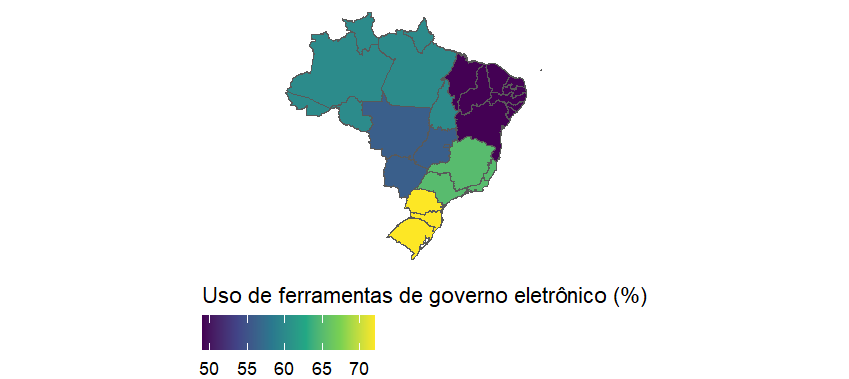
\includegraphics[width=1\linewidth]{figuras/mapa_coropletico_tic_domicilios_2024_g1}
	\label{fig:mapa_coropletico_tic_domicilio_g1}
	\footnotesize{Fonte: \cite{tic_domicilios_2024_g1}.}
\end{figure}

A figura \ref{fig:mapa_coropletico_tic_domicilio_g1} representa os resultados do indicador G1. As regiões Sul e Sudeste são as regiões que mais usam o governo eletrônico, seguidas das regiões Centro-Oeste e Norte. Por último, está o Nordeste.

O indicador G2 complementa o G1 ao especificar quais grupos de funções de governo eletrônico foram os mais usados. O indicador G2 tem os seguintes critérios:

\begin{itemize}
	\item Documentos pessoais, como RG, CPF, passaporte ou carteira de trabalho (G2-1)
	Saúde pública, como agendamento de consultas, remédios ou outros serviços do sistema público de saúde (G2-2).
	\item Educação pública, como Enem, Prouni, matrículas em escolas ou universidades públicas (G2-3).
	\item Direito do trabalhador ou previdência social, como INSS, FGTS, seguro-desemprego, auxílio-doença ou aposentadoria (G2-4).
	\item Impostos e taxas governamentais, como declaração de imposto de renda, IPVA ou IPTU (G2-5).
	\item Polícia e segurança, como boletim de ocorrência, antecedentes criminais ou denúncias (G2-6).
	\item Transporte público ou outros serviços urbanos, como limpeza e conservação de vias, iluminação (G2-7).
\end{itemize}

As figuras seguintes detalham como cada critério é usado por região.

\begin{figure}[H]
	\centering
	\caption{Indicador G2: critérios 1 e 2 (em \%)}
	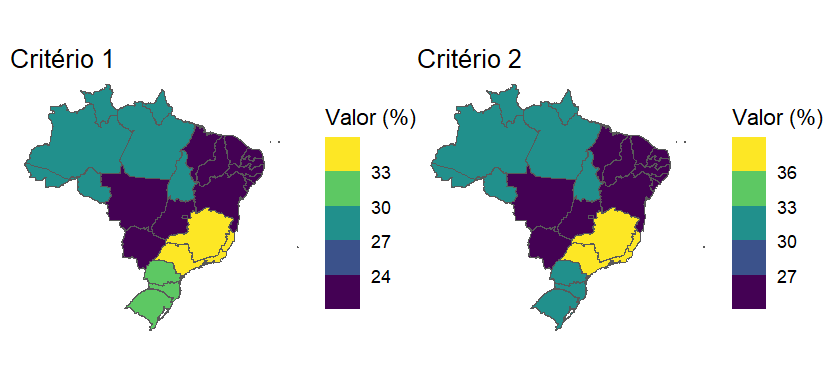
\includegraphics[width=1\linewidth]{figuras/mapa_coropletico_tic_domicilios_2024_g2_1_2.png}
	\label{fig:mapa_coropletico_tic_domicilios_2024_g2_1_2}
	\footnotesize{Fonte: \cite{tic_domicilios_2024_g2}.}
\end{figure}

Quando se trata do indicador G2-1, as regiões que mais buscaram serviços públicos relativos a documentos pessoais, como RG, CPF, passaporte ou carteira de trabalho foram as Norte, Sudeste e Sul;

Quando se trata do indicador G2-2, apenas o Nordeste foi a região que menos uso serviços públicos relativos à saúde pública, como agendamento de consultas, remédios ou outros serviços do sistema público de saúde.

\begin{figure}[H]
	\centering
	\caption{Indicador G2: critérios 3 e 4 (em \%)}
	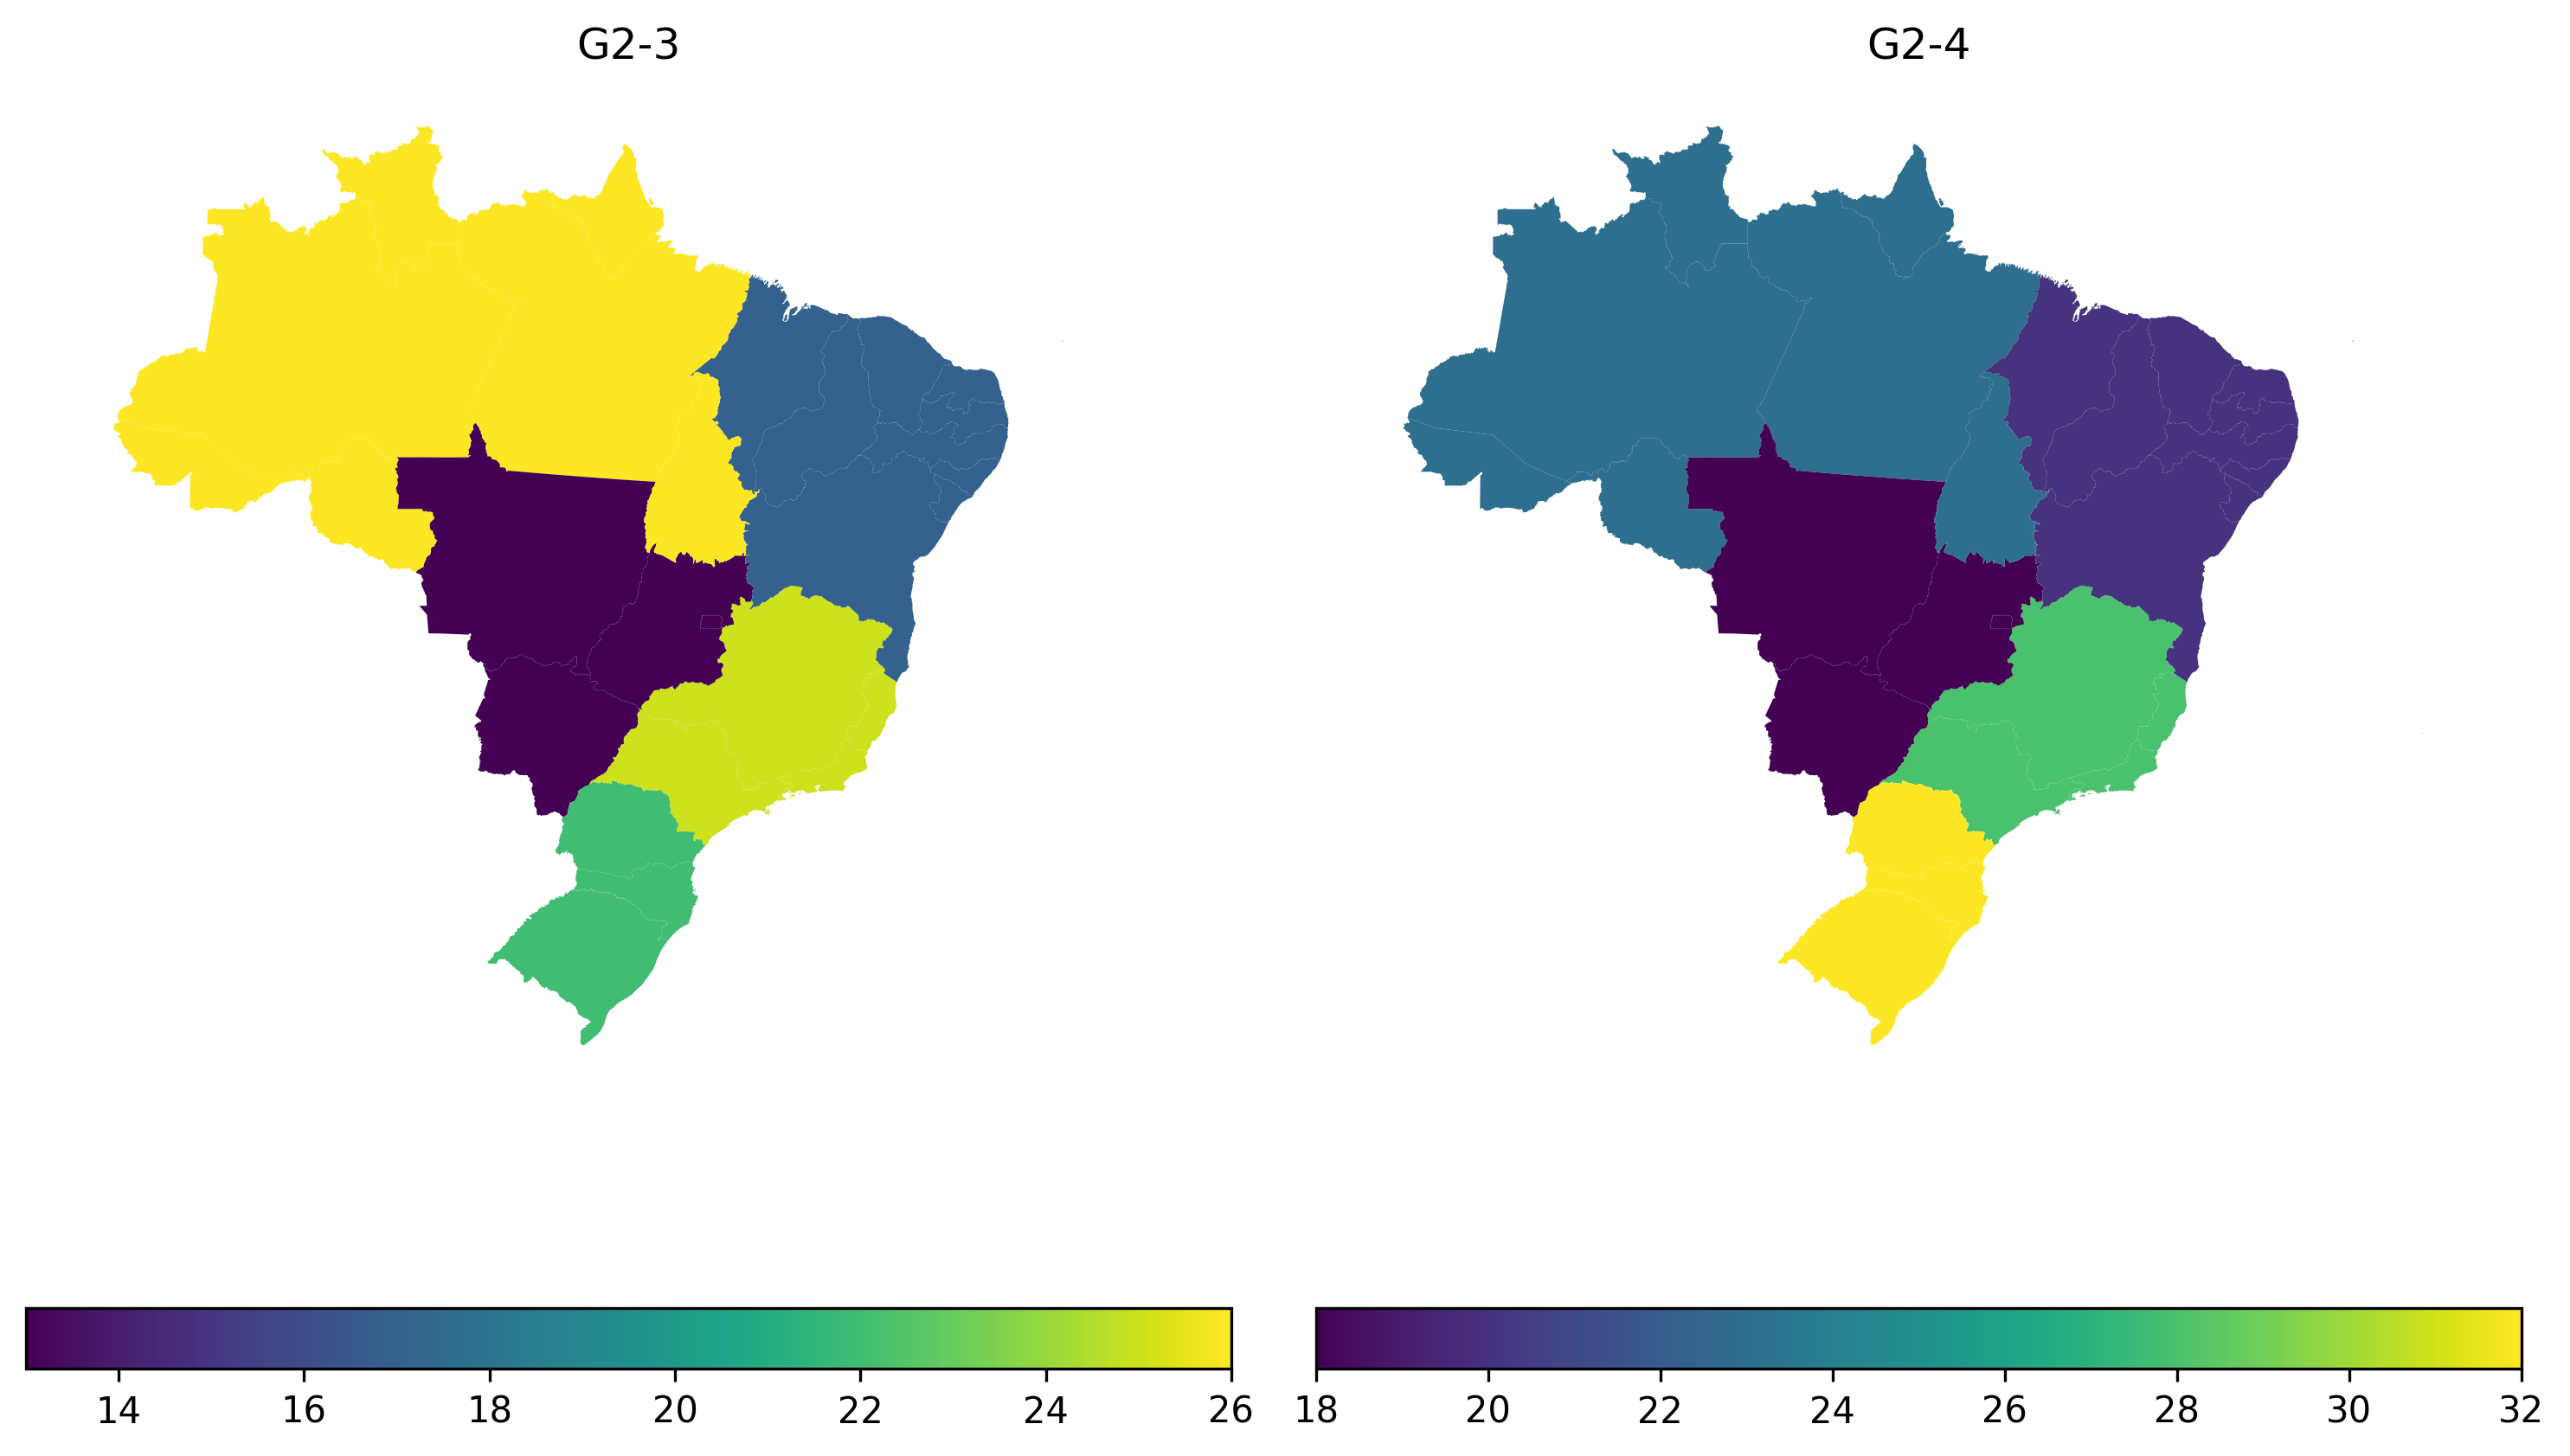
\includegraphics[width=1\linewidth]{figuras/mapa_coropletico_tic_domicilios_2024_g2_3_4.png}
	\label{fig:mapa_coropletico_tic_domicilios_2024_g2_3_4}
	\footnotesize{Fonte: \cite{tic_domicilios_2024_g2}.}
\end{figure}

Quando se trata do indicador G2-3, as regiões que mais usam serviços públicos relativos à educação pública, como Enem, Prouni, matrículas em escolas ou universidades públicas foram a Norte e a Sudeste.

Quando se trata do indicador G2-4, as regiões que mais usar serviços públicos relativos ao direito do trabalhador ou previdência social, como INSS, FGTS, seguro-desemprego, auxílio-doença ou aposentadoria foram as Sudeste e a Sul.

\begin{figure}[H]
	\centering
	\caption{Indicador G2: critérios 5 e 6 (em \%)}
	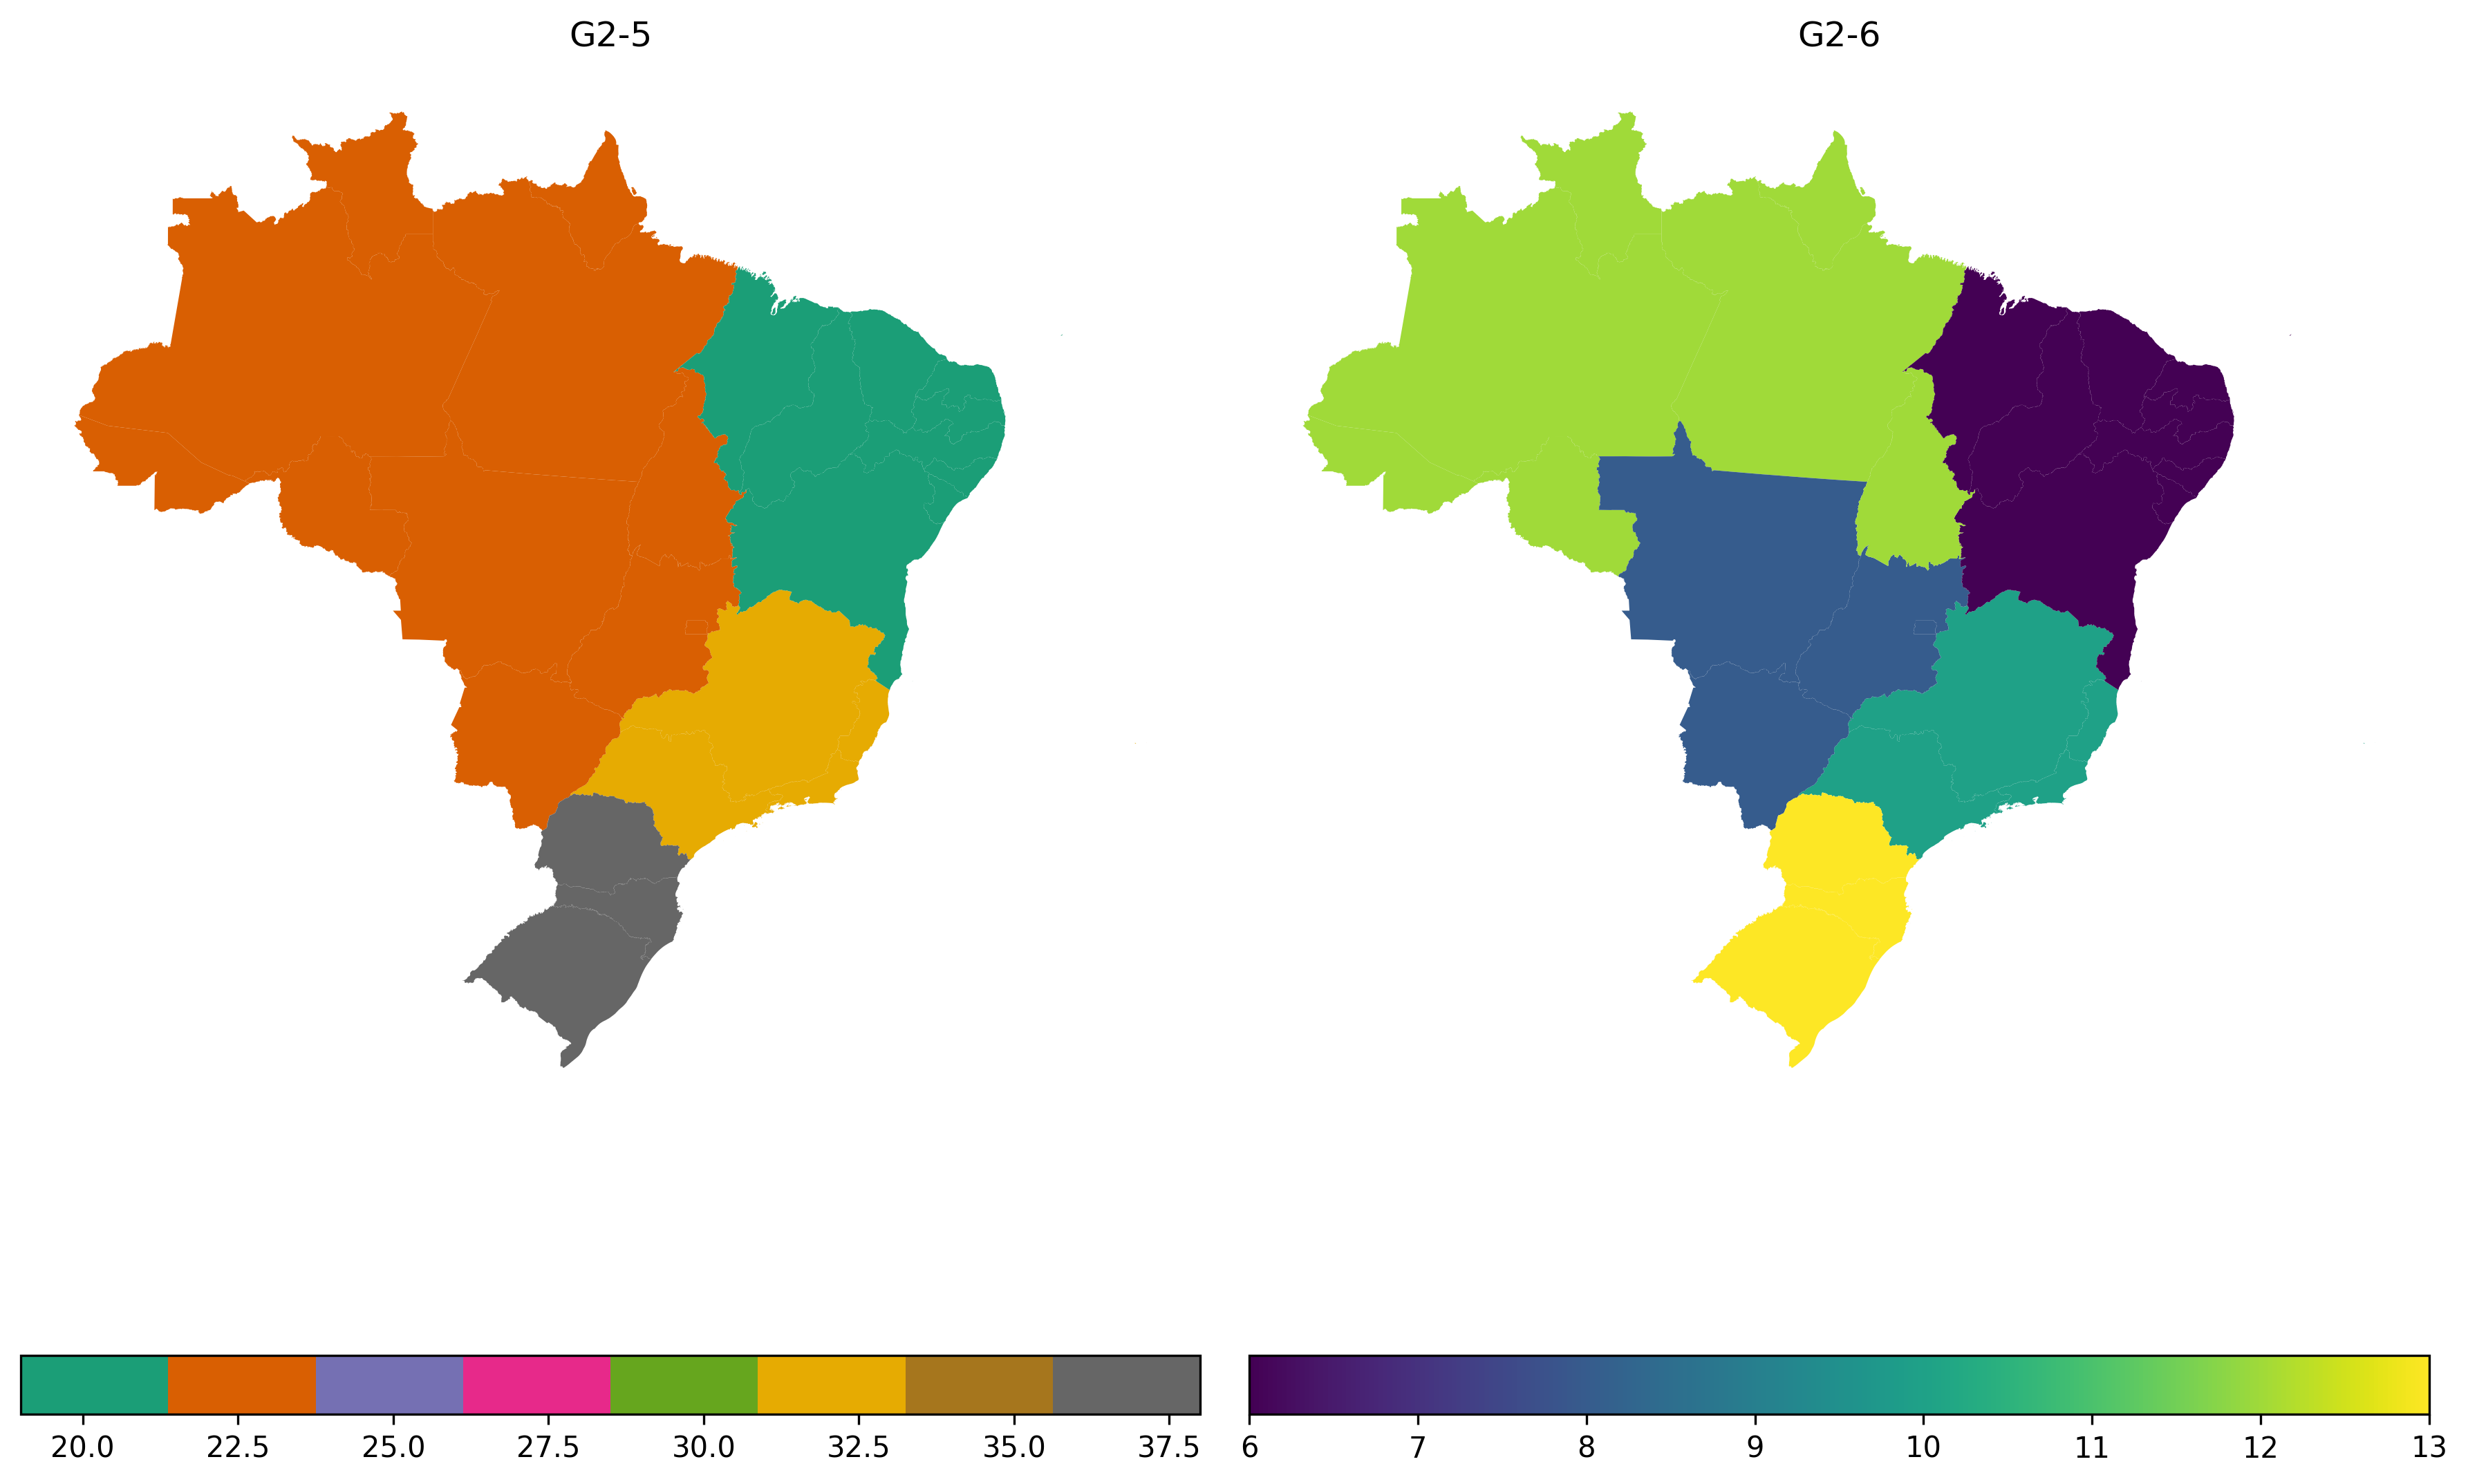
\includegraphics[width=1\linewidth]{figuras/mapa_coropletico_tic_domicilios_2024_g2_5_6.png}
	\label{fig:mapa_coropletico_tic_domicilios_2024_g2_5_6}
	\footnotesize{Fonte: \cite{tic_domicilios_2024_g2}.}
\end{figure}

Quando se trata do indicador G2-5, apenas as regiões Sudeste e Sul foram as que mais usaram serviços públicos relativos a impostos e taxas governamentais, como declaração de imposto de renda, IPVA ou IPTU.

Quando se trata do indicador G2-6, apenas a região Sul foi a que mais usou serviços públicos relativos à polícia e segurança, como boletim de ocorrência, antecedentes criminais ou denúncias.

\begin{figure}[H]
	\centering
	\caption{Indicador G2: critério 7 (em \%)}
	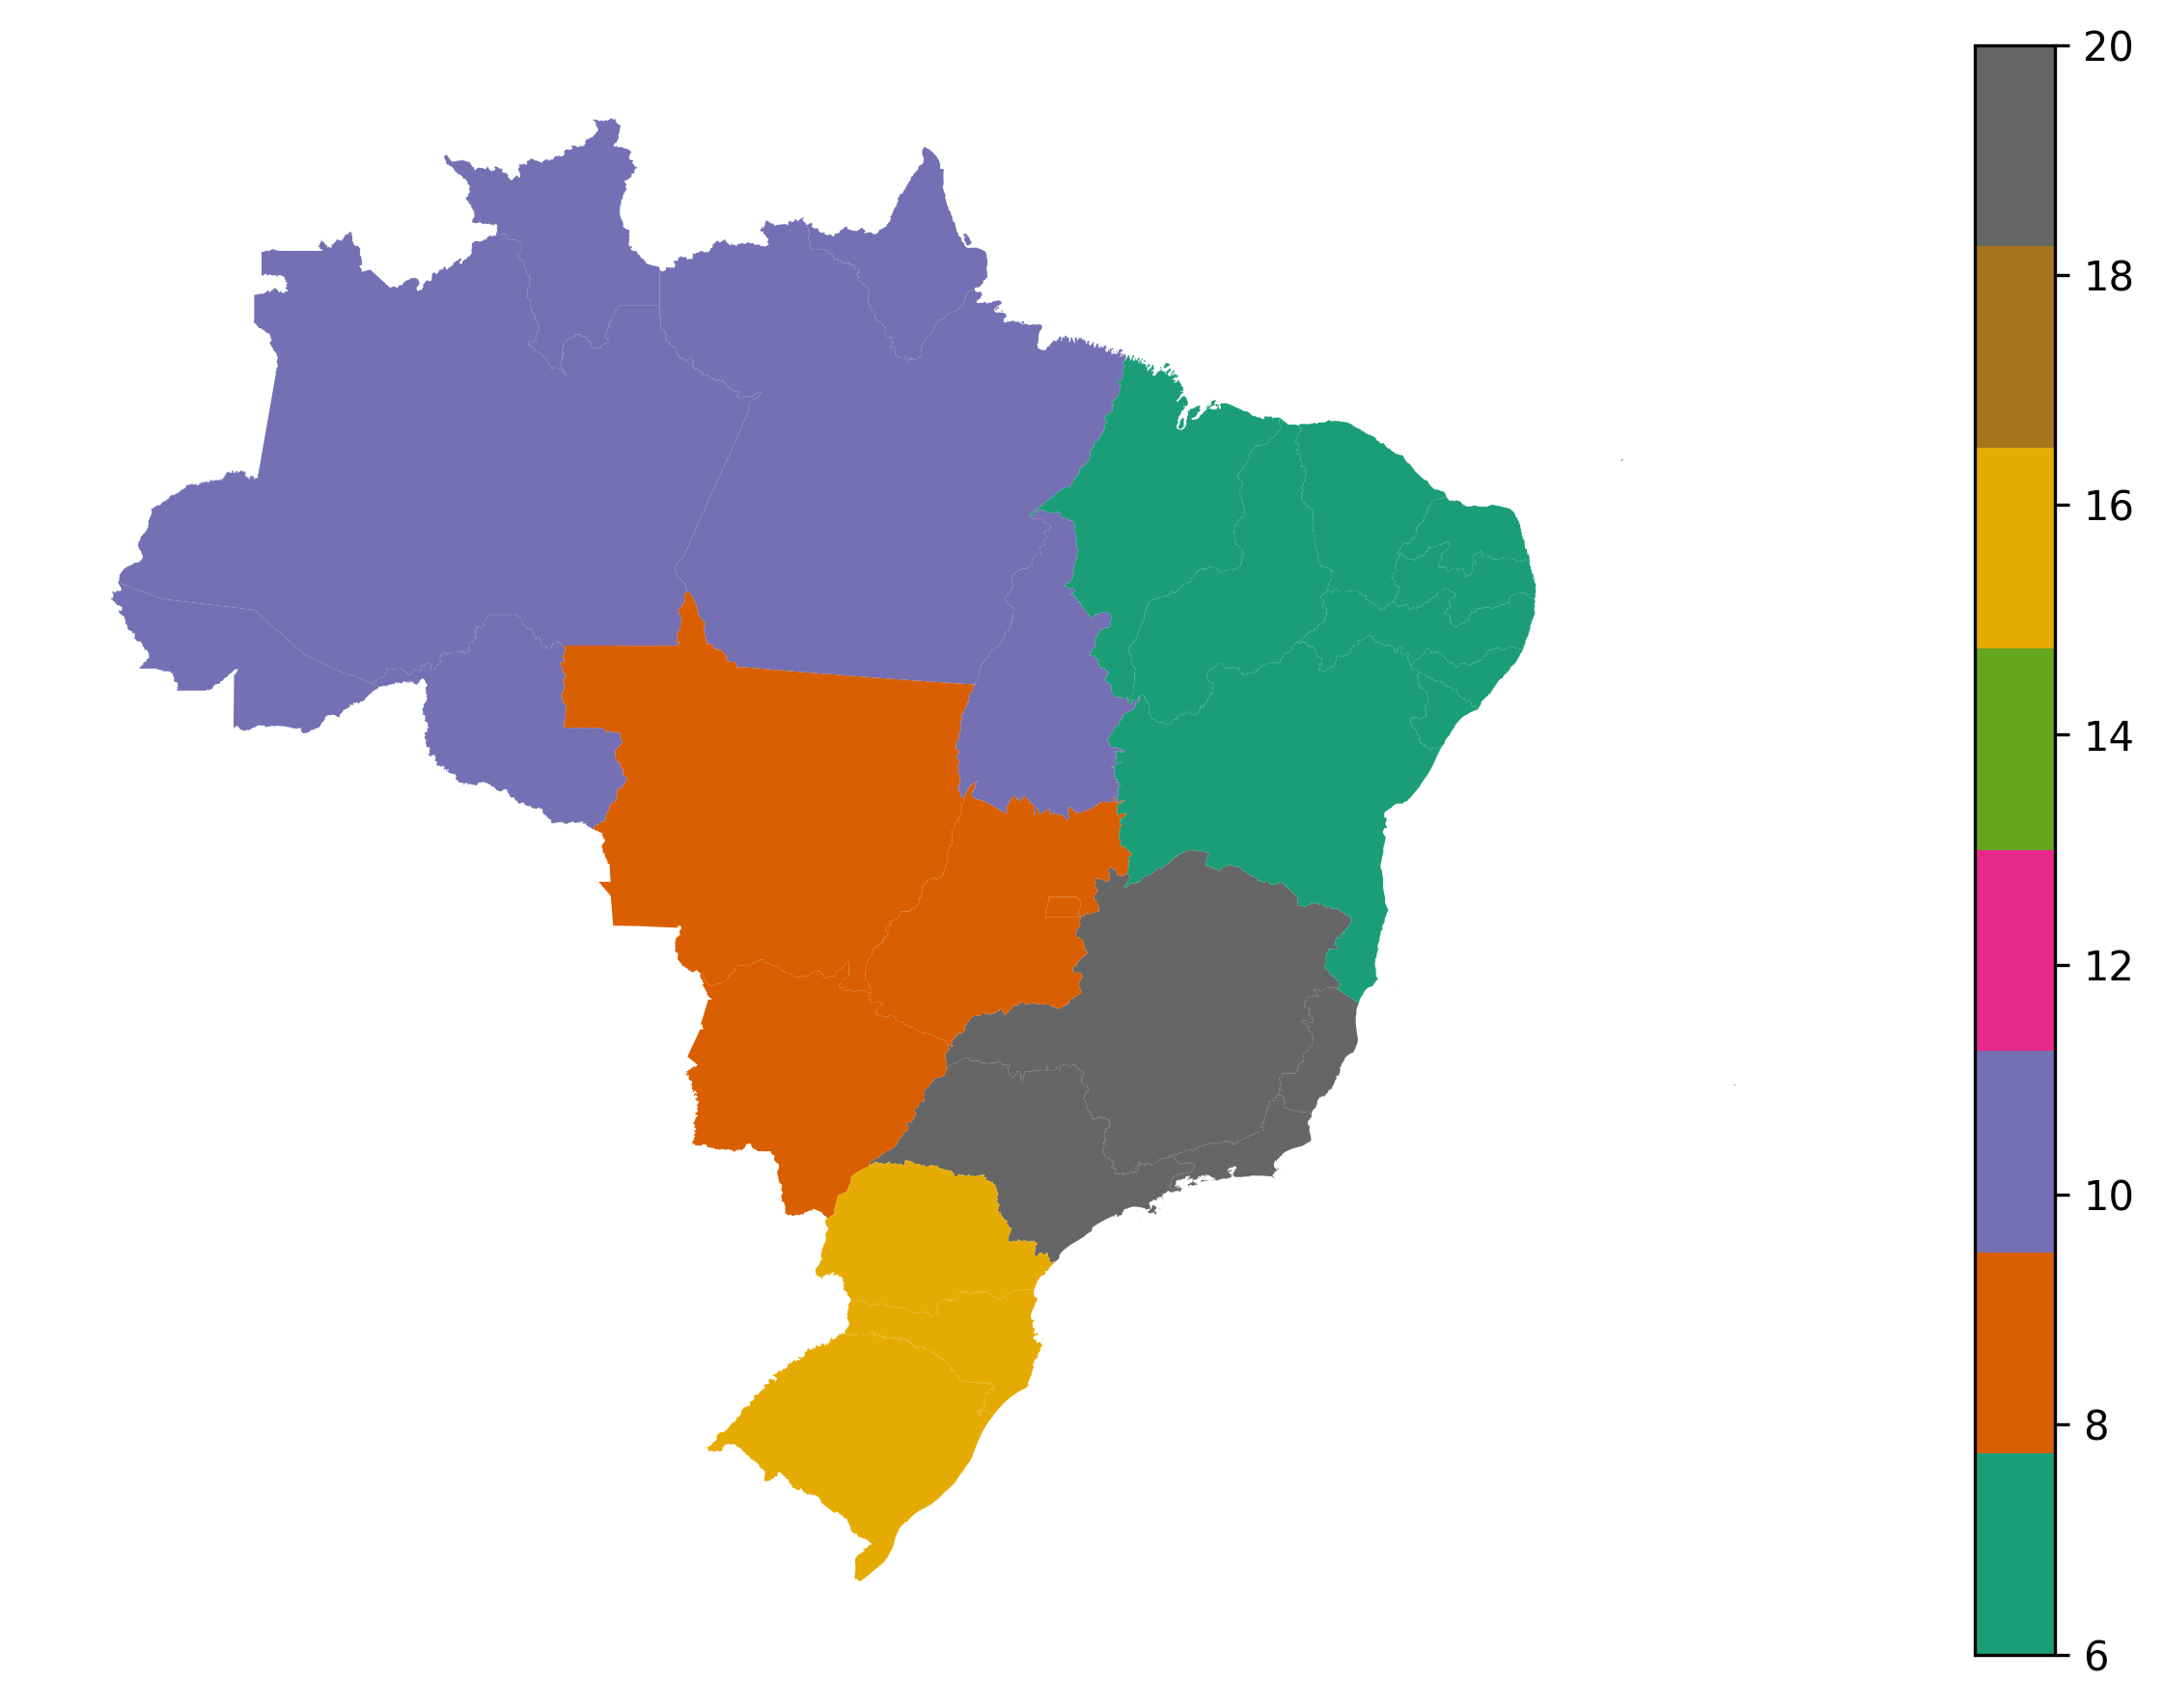
\includegraphics[width=1\linewidth]{figuras/mapa_coropletico_tic_domicilios_2024_g2_7.png}
	\label{fig:mapa_coropletico_tic_domicilios_2024_g2_7}
	\footnotesize{Fonte: \cite{tic_domicilios_2024_g2}.}
\end{figure}

Quando se trata do indicador G2-7, as regiões Sudeste e Sul foram as únicas que mais usaram serviços públicos relativos a transporte público ou outros serviços urbanos, como limpeza e conservação de vias e iluminação.

Complementar ao indicador G2, o indicador G2A detalha se o serviço público foi realizado, completamente ou parcialmente, na internet, e se apenas informações do serviço público foram procuradas na internet, incluídas as opções em que o questionado não respondeu ou não sabe, todos como subcritérios. 

O indicador G2A tem 7 critérios, conforme exposto abaixo:

\begin{itemize}
	\item Documentos pessoais, como RG, CPF, passaporte ou carteira de trabalho.
	Saúde pública, como agendamento de consultas, remédios ou outros serviços do sistema público de saúde.
	\item Educação pública, como Enem, Prouni, matrículas em escolas ou universidades públicas.
	\item Direito do trabalhador ou previdência social, como INSS, FGTS, seguro-desemprego, auxílio-doença ou aposentadoria.
	\item Impostos e taxas governamentais, como declaração de imposto de renda, IPVA ou IPTU.
	\item Polícia e segurança, como boletim de ocorrência, antecedentes criminais ou denúncias.
	\item Transporte público ou outros serviços urbanos, como limpeza e conservação de vias, iluminação.
\end{itemize}

Os subcritérios do indicador G2A são, segundo \cite{tic_domicilios_2024_g2a}:

\begin{itemize}
    \item Realizou serviço na Internet sem precisar ir até um posto (SC1);  \item Realizou parte do serviço na Internet, mas precisou ir a um posto para finalizar (SC2);
    \item Apenas procurou informações na Internet (SC3);
    \item Não sabe; e
    \item Não respondeu.
\end{itemize}

As figuras \ref{fig:mapa_coropletico_tic_domicilios_2024_g2a_1}, \ref{fig:mapa_coropletico_tic_domicilios_2024_g2a_2}, \ref{fig:mapa_coropletico_tic_domicilios_2024_g2a_3},
\ref{fig:mapa_coropletico_tic_domicilios_2024_g2a_4},
\ref{fig:mapa_coropletico_tic_domicilios_2024_g2a_5} contêm mapa coropléticos que demonstram os subcritérios dos indicadores do G2A, que não incluirão as opções \textbf{não respondeu} e \textbf{não sabe}.

\begin{figure}[H]
	\centering
	\caption{Indicador G2A: critério 1 (em \%)}
	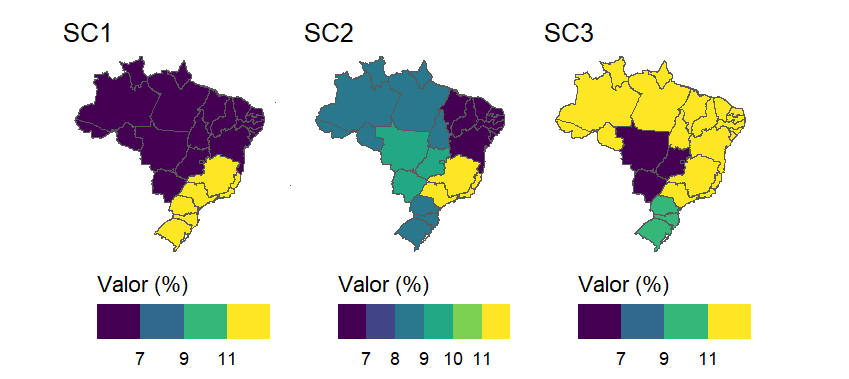
\includegraphics[width=1\linewidth]{figuras/mapa_coropletico_tic_domicilios_2024_g2a_1.png}
	\label{fig:mapa_coropletico_tic_domicilios_2024_g2a_1}
	\footnotesize{Fonte: \cite{tic_domicilios_2024_g2a}.}
\end{figure}

No tocante ao SC1, as regiões Sudeste e Sul foram as regiões em que mais ocorreram serviços na internet sem precisar ir até um posto. 

No tocante ao SC2, a região Sudeste foi a única região em que mais foram realizados partes dos serviços na Internet, mas foi preciso ir a um posto para finalizar, seguida do Centro-Oeste e das regiões Norte e Sul.

No tocante ao SC3, as regiões Norte, Nordeste, Sudeste foram as regiões em que mais se procurou informações na internet, seguidas do Sul e do Centro-Oeste.

\begin{figure}[H]
	\centering
	\caption{Indicador G2A: critério 2 (em \%)}
	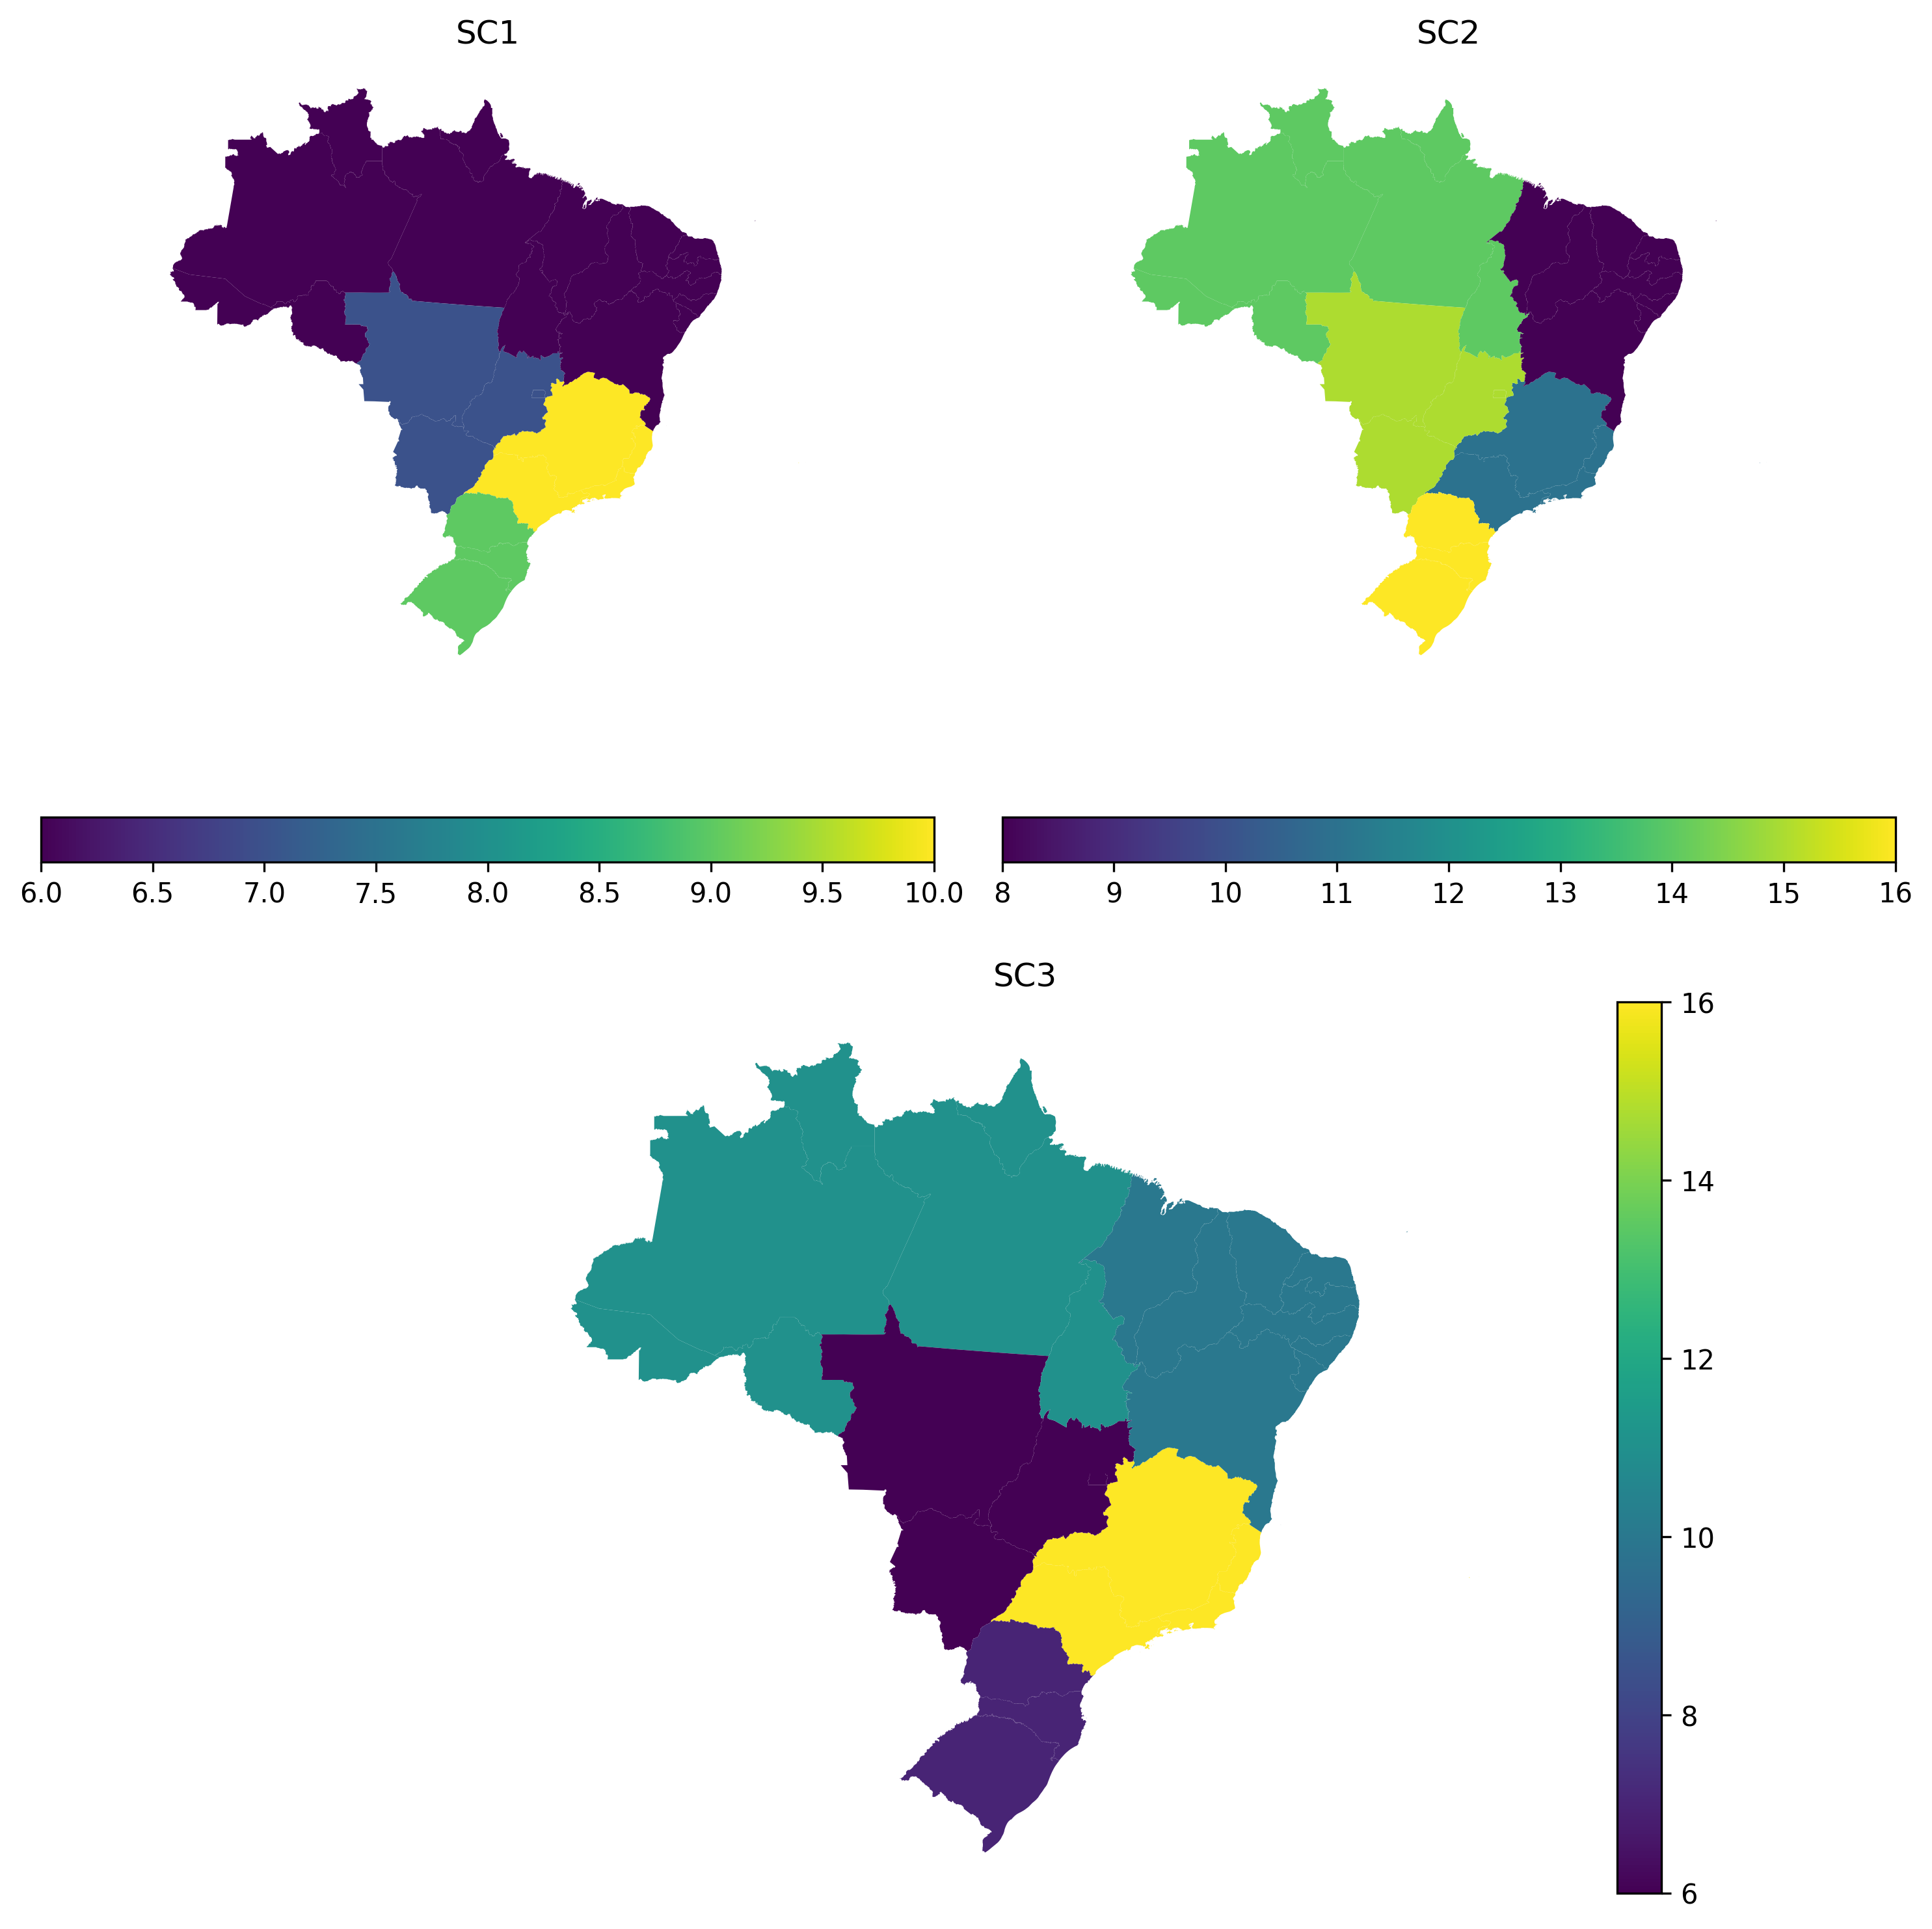
\includegraphics[width=1\linewidth]{figuras/mapa_coropletico_tic_domicilios_2024_g2a_2.png}
	\label{fig:mapa_coropletico_tic_domicilios_2024_g2a_2}
	\footnotesize{Fonte: \cite{tic_domicilios_2024_g2a}.}
\end{figure}

No tocante ao SC1, as regiões Sudeste e Sul foram as regiões em que mais ocorreram serviços na internet sem precisar ir até um posto.

No tocante ao SC2, a região Sudeste foi a região em que mais foram realizados partes dos serviços na Internet, mas foi preciso ir a um posto para finalizar, seguidas  das regiões Sul e Norte, e por fim, do Centro-Oeste.

No tocante ao SC3, a região Sudeste foi a região em que mais se procurou informações na internet, seguida do Nordeste e Norte, bem como, conjuntamente, o Centro-Oeste e o Sul.

\begin{figure}[H]
	\centering
	\caption{Indicador G2A: critério 3 (em \%)}
	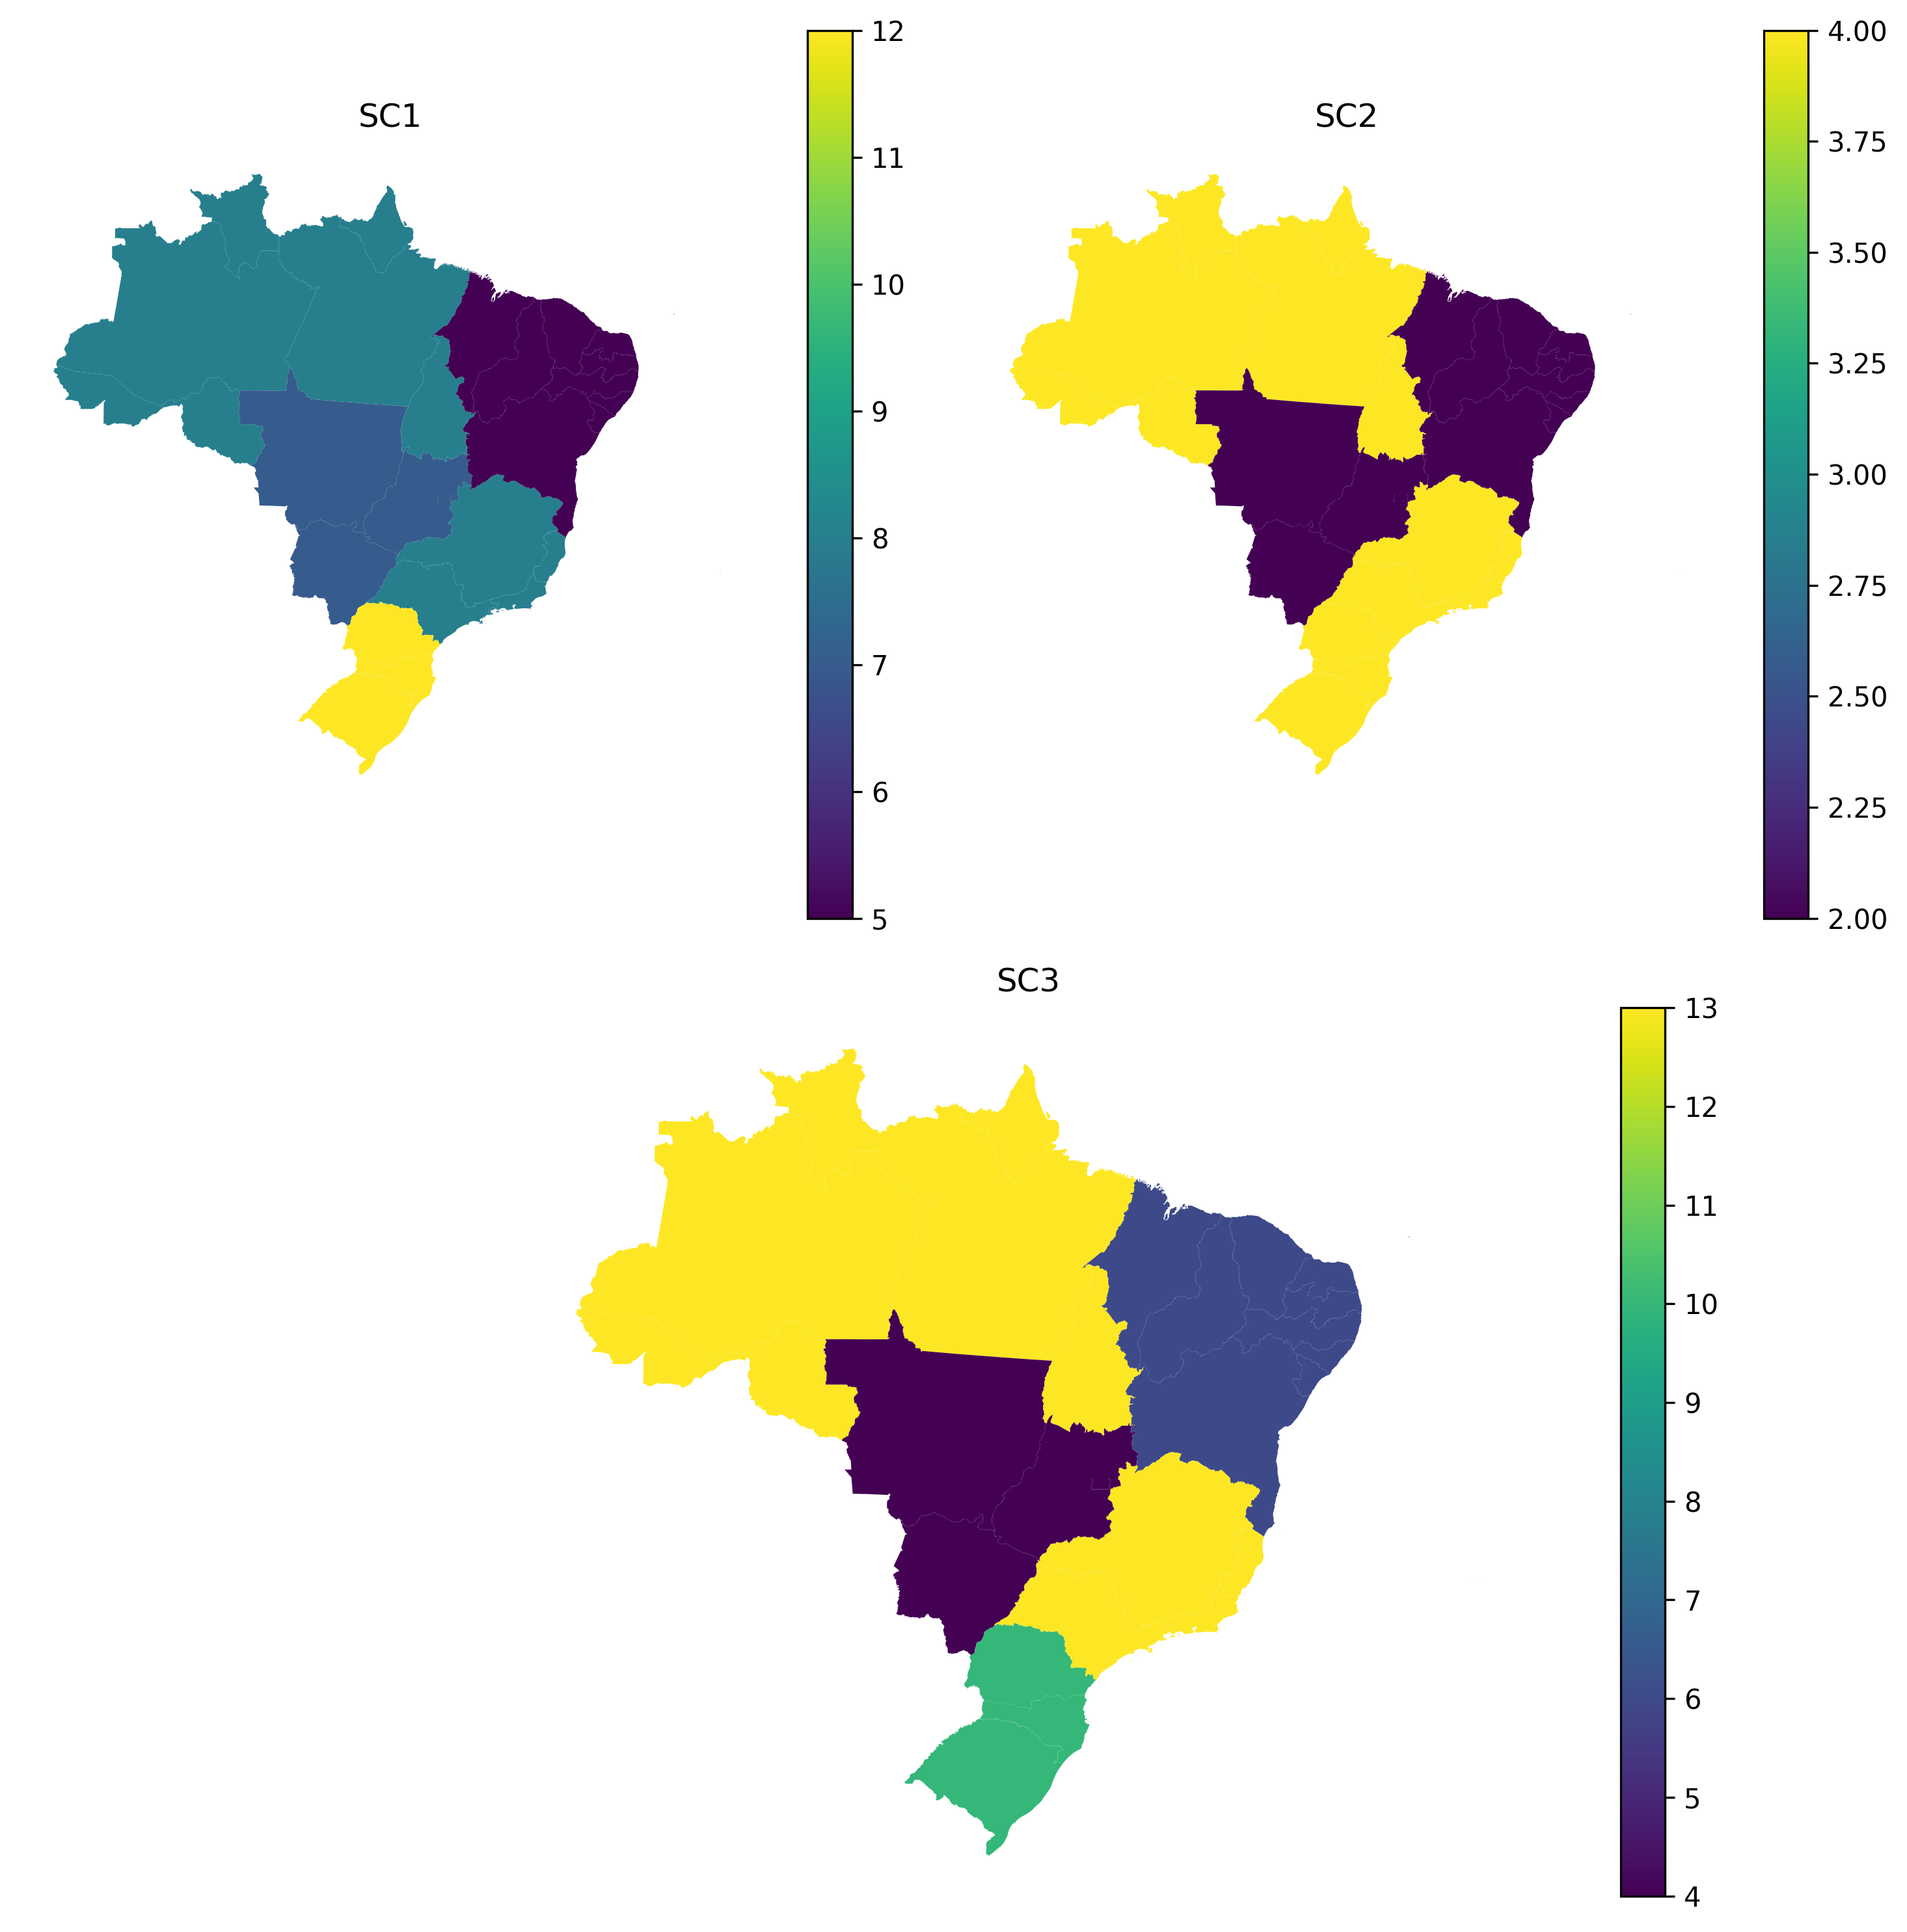
\includegraphics[width=1\linewidth]{figuras/mapa_coropletico_tic_domicilios_2024_g2a_3.png}
	\label{fig:mapa_coropletico_tic_domicilios_2024_g2a_3}
	\footnotesize{Fonte: \cite{tic_domicilios_2024_g2a}.}
\end{figure}

No tocante ao SC1, a região Sul foi a região em que mais ocorreram serviços na internet sem precisar ir até um posto, sendo o Nordeste a região em que mais se foi presencialmente aos postos.

No tocante ao SC2, as regiões Norte, Sudeste e Sul foram as regiões em que mais foram realizados partes dos serviços na Internet, mas foi preciso ir a um posto para finalizar, seguidas do Nordeste e Centro-Oeste.

No tocante ao SC3, as regiões Norte e Sudeste em que mais se procurou informações na internet, seguidas do Nordeste e das regiões Centro-Oeste e Sul.

\begin{figure}[H]
	\centering
	\caption{Indicador G2A: critério 4 (em \%)}
	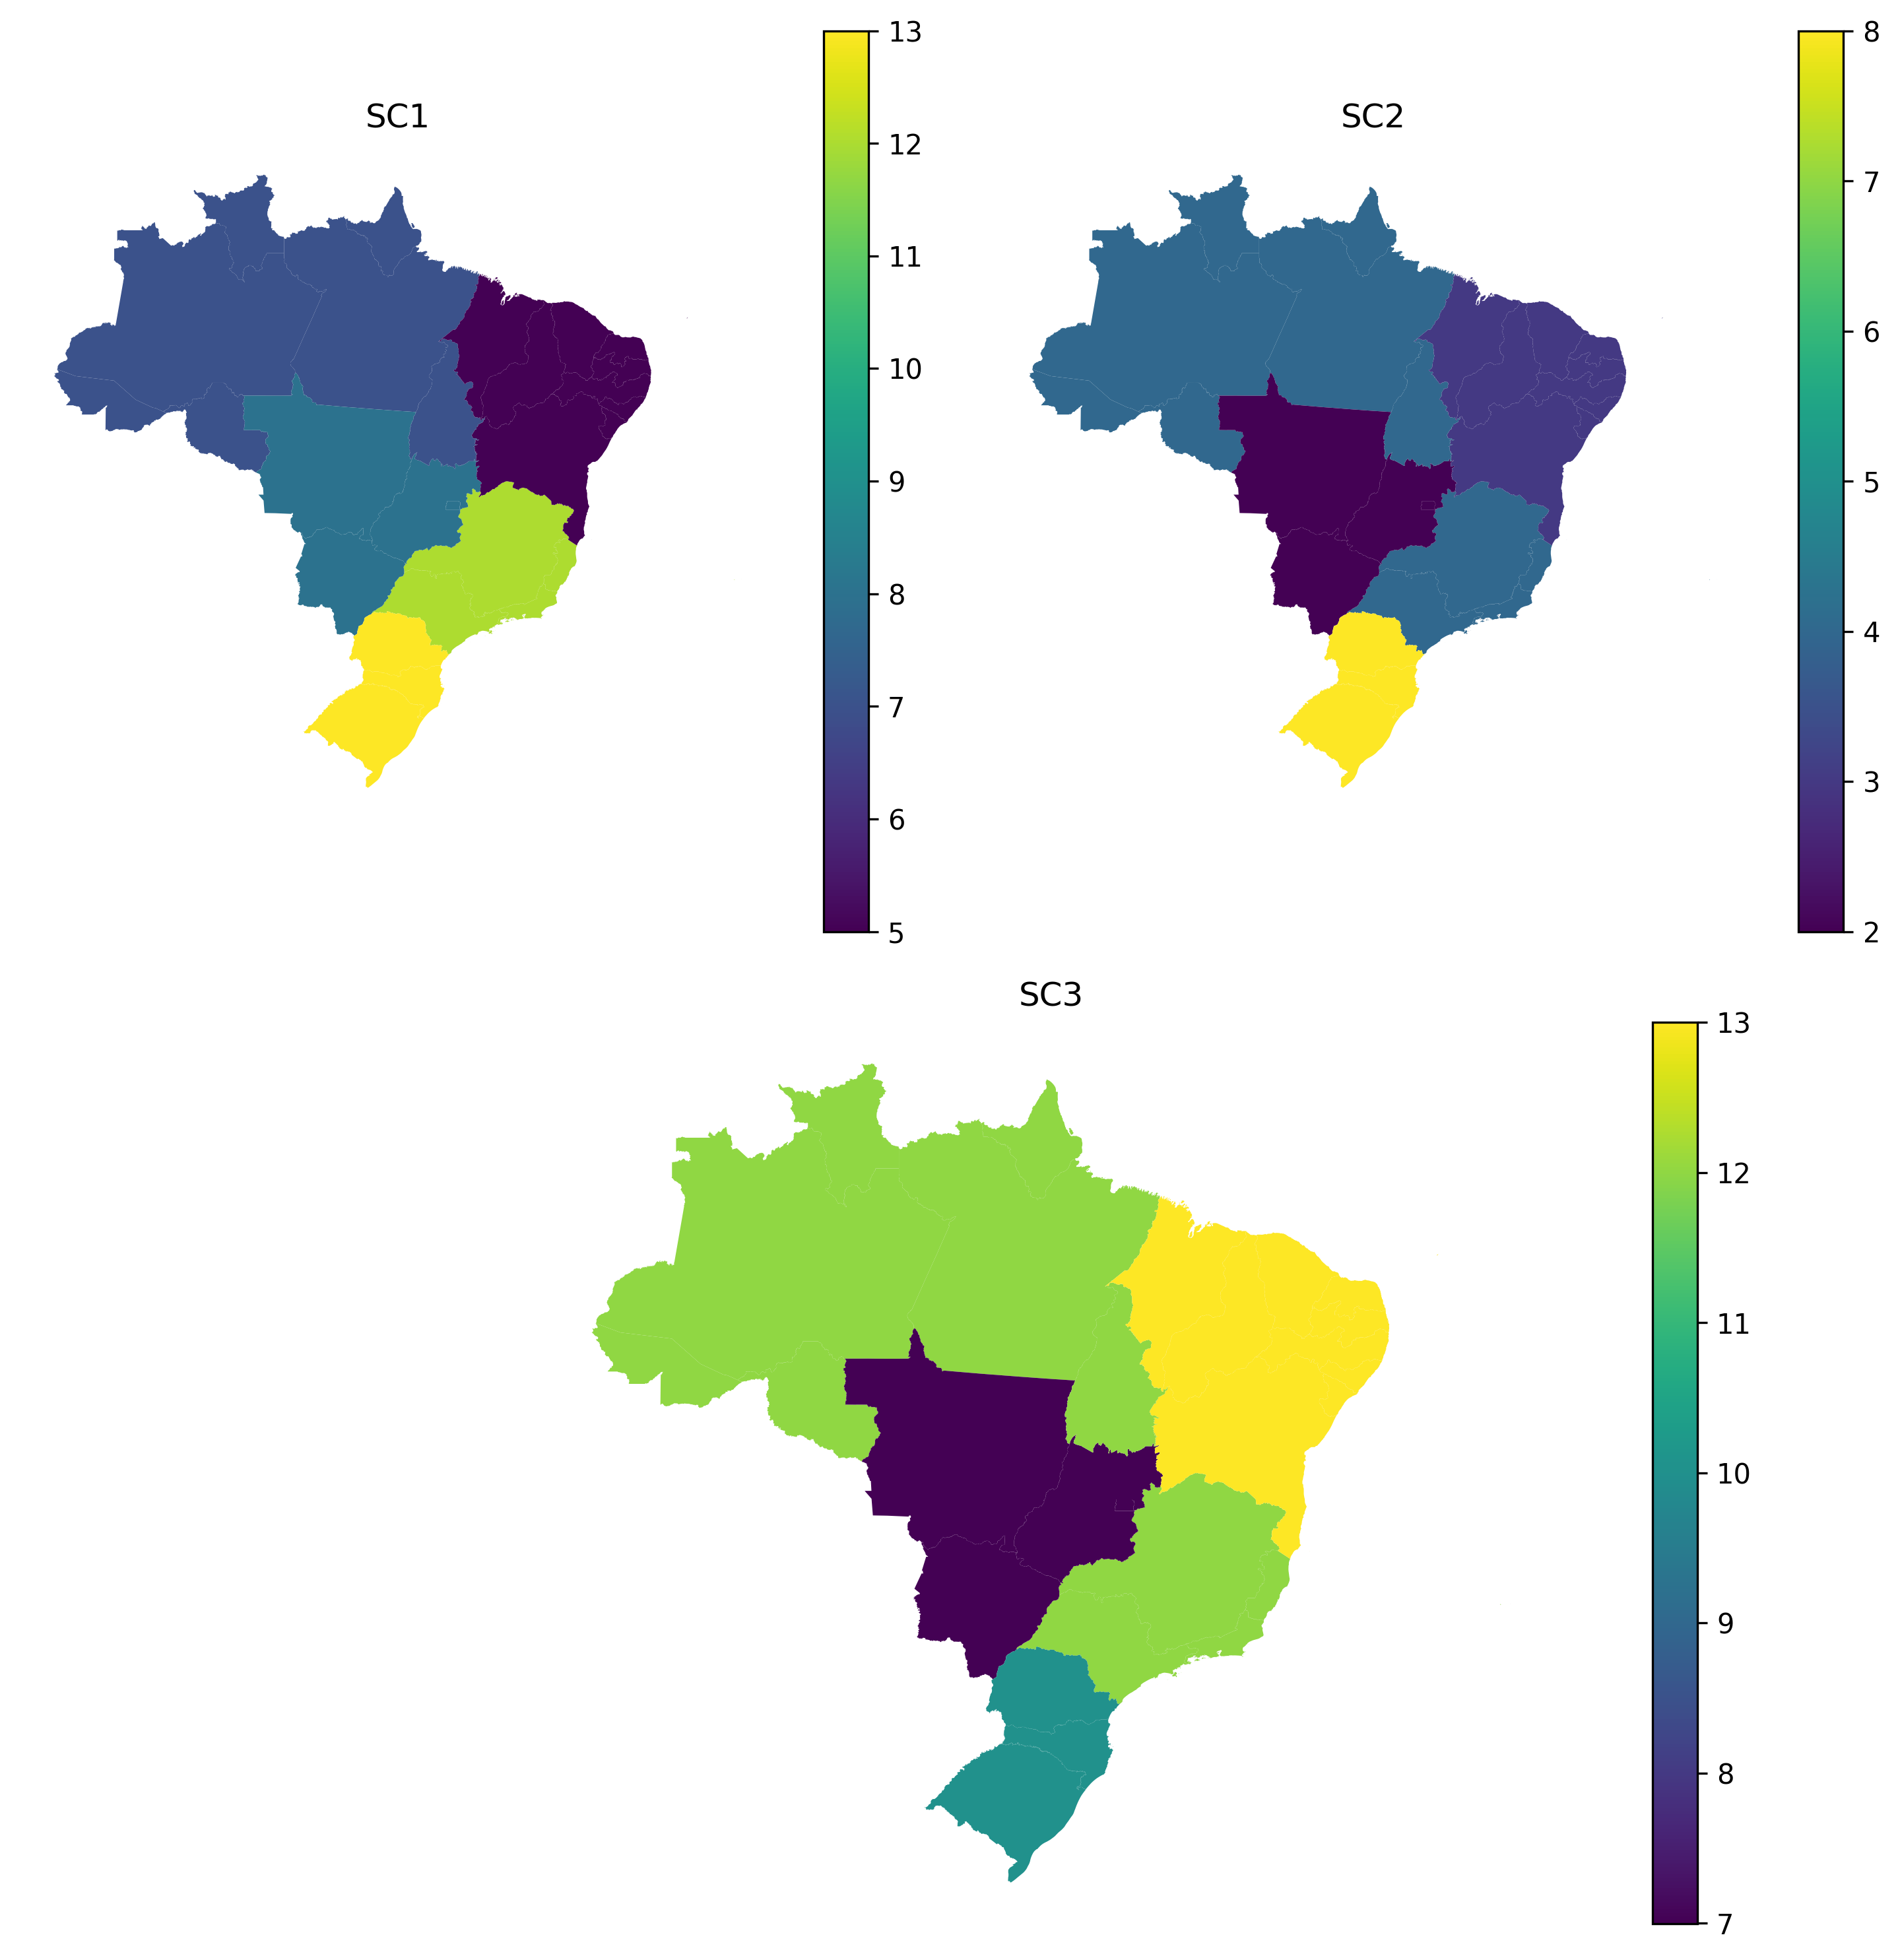
\includegraphics[width=1\linewidth]{figuras/mapa_coropletico_tic_domicilios_2024_g2a_4.png}
	\label{fig:mapa_coropletico_tic_domicilios_2024_g2a_4}
	\footnotesize{Fonte: \cite{tic_domicilios_2024_g2a}.}
\end{figure}

No tocante ao SC1, as regiões Sudeste e Sul foram as regiões em que mais ocorreram serviços na internet sem precisar ir até um posto, seguidas do Centro-Oeste e das regiões Norte e Nordeste.

No tocante ao SC2, a região Sul foi a região em que mais foram realizados partes dos serviços na Internet, mas foi preciso ir a um posto para finalizar, seguidas do Sudeste e Norte e das regiões Centro-Oeste e Nordeste.

No tocante ao SC3, a região Nordeste foi a região em que mais se procurou informações na internet, seguidas do Norte e Sudeste e da região Centro-Oeste.

\begin{figure}[H]
	\centering
	\caption{Indicador G2A: critério 5 (em \%)}
	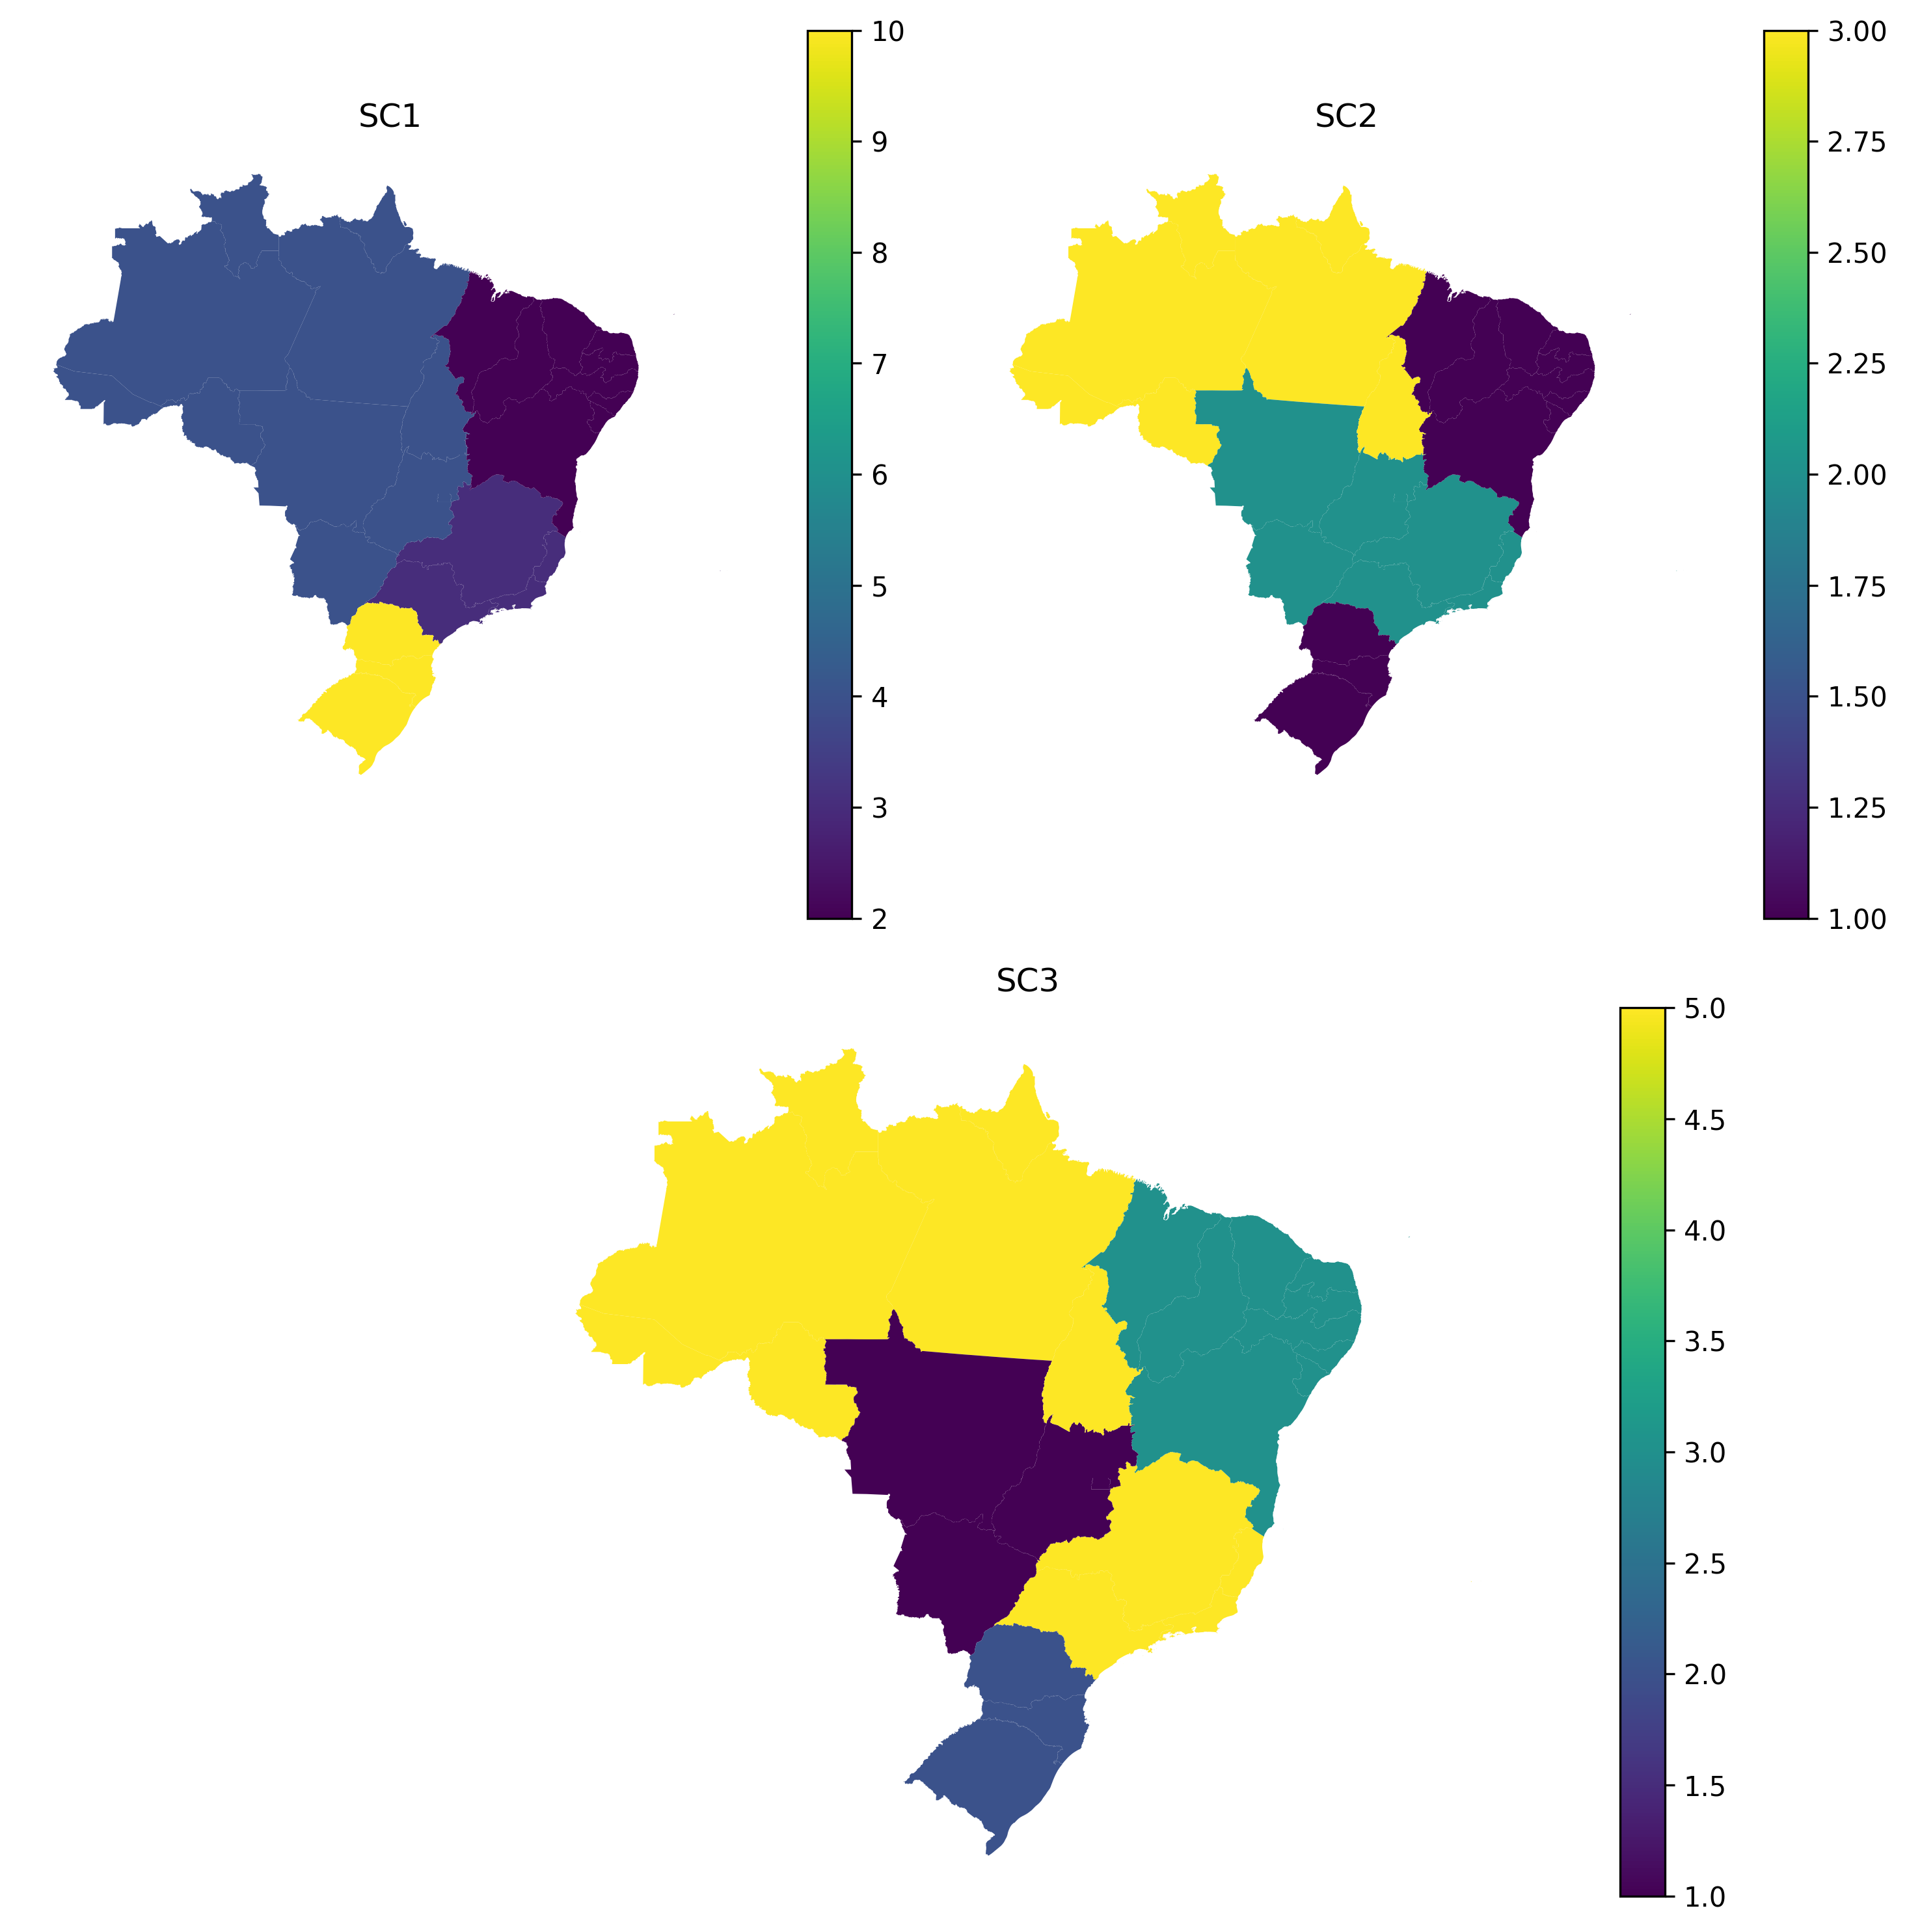
\includegraphics[width=1\linewidth]{figuras/mapa_coropletico_tic_domicilios_2024_g2a_5.png}
	\label{fig:mapa_coropletico_tic_domicilios_2024_g2a_5}
	\footnotesize{Fonte: \cite{tic_domicilios_2024_g2a}.}
\end{figure}

No tocante ao SC1, a região Sul foi a região em que mais ocorreram serviços na internet sem precisar ir até um posto, seguidas do Sudeste, Centro-Oeste e das regiões Norte e Nordeste.

No tocante ao SC2, a região Sul foi a região em que mais foram realizados partes dos serviços na Internet, mas foi preciso ir a um posto para finalizar, seguidas do Centro-Oeste e Norte e das regiões Sudeste e Nordeste.

No tocante ao SC3, as regiões Norte e Nordeste foram a região em que mais se procurou informações na internet, seguidas do Sudeste, Sul e da região Centro-Oeste.

\begin{figure}[H]
	\centering
	\caption{Indicador G2A: critério 6 (em \%)}
	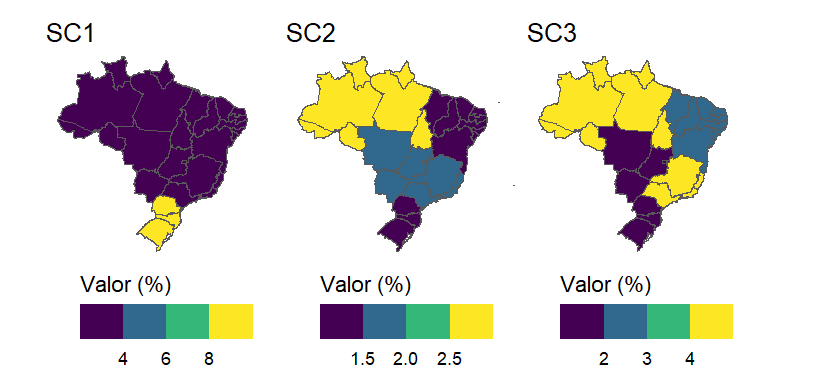
\includegraphics[width=1\linewidth]{figuras/mapa_coropletico_tic_domicilios_2024_g2a_6.png}
	\label{fig:mapa_coropletico_tic_domicilios_2024_g2a_6}
	\footnotesize{Fonte: \cite{tic_domicilios_2024_g2a}.}
\end{figure}

No tocante ao SC1, apenas a região Sul foi a região em que mais ocorreram serviços na internet sem precisar ir até um posto.

No tocante ao SC2, a região Norte foi a região em que mais foram realizados partes dos serviços na Internet, mas foi preciso ir a um posto para finalizar, seguidas do Centro-Oeste e Sudeste e das regiões Sul e Nordeste.

No tocante ao SC3, as regiões Norte e Sudeste foram a região em que mais se procurou informações na internet, seguidas do Nordeste e das regiões Centro-Oeste e Sul.

\begin{figure}[H]
	\centering
	\caption{Indicador G2A: critério 7 (em \%)}
	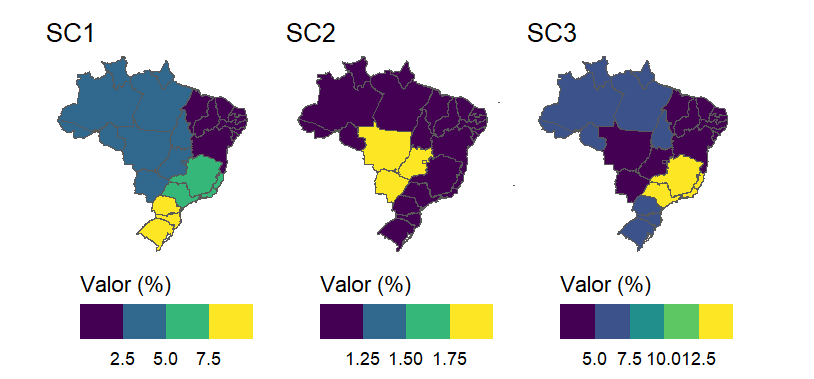
\includegraphics[width=1\linewidth]{figuras/mapa_coropletico_tic_domicilios_2024_g2a_7.png}
	\label{fig:mapa_coropletico_tic_domicilios_2024_g2a_7}
	\footnotesize{Fonte: \cite{tic_domicilios_2024_g2a}.}
\end{figure}

No tocante ao SC1, a região Sul foi a região em que mais ocorreram serviços na internet sem precisar ir até um posto, seguidas das regiões Sudeste, conjuntamente, o Centro-Oeste e o Norte, e por fim, o Nordeste.

No tocante ao SC2, apenas a região Centro-Oeste foi a região em que mais foram realizados partes dos serviços na Internet.

No tocante ao SC3, as regiões Norte e Sudeste foram a região em que mais se procurou informações na internet, seguidas do Nordeste e das regiões Centro-Oeste e Sul.

Terminando a análise do TIC Domicílios 2024, analisar-se-á o indicador G3. O indicador representa os usuários de internet, por atividades de interação com autoridades públicas.

A lista abaixo contém a tabela com a descrição dos seus 3 critérios.  

\begin{itemize}
	\item Procurou informações oferecidas por sites de governo (C1).
	\item Realizou algum serviço público, como emitir documentos pela Internet, preencher e enviar formulários online ou pagar taxas e impostos pela Internet (C2).
	\item Não utilizou a Internet para realizar atividades de interação com autoridades públicas (C3).
\end{itemize}

Haja vista a lista acima, a figura \ref{fig:mapa_coropletico_tic_domicilios_2024_g3}  representa o percentual de usuários de internet, por atividades de interação com autoridades públicas. 

\begin{figure}[H]
	\centering
	\caption{Indicador G3: critérios (em \%)}
	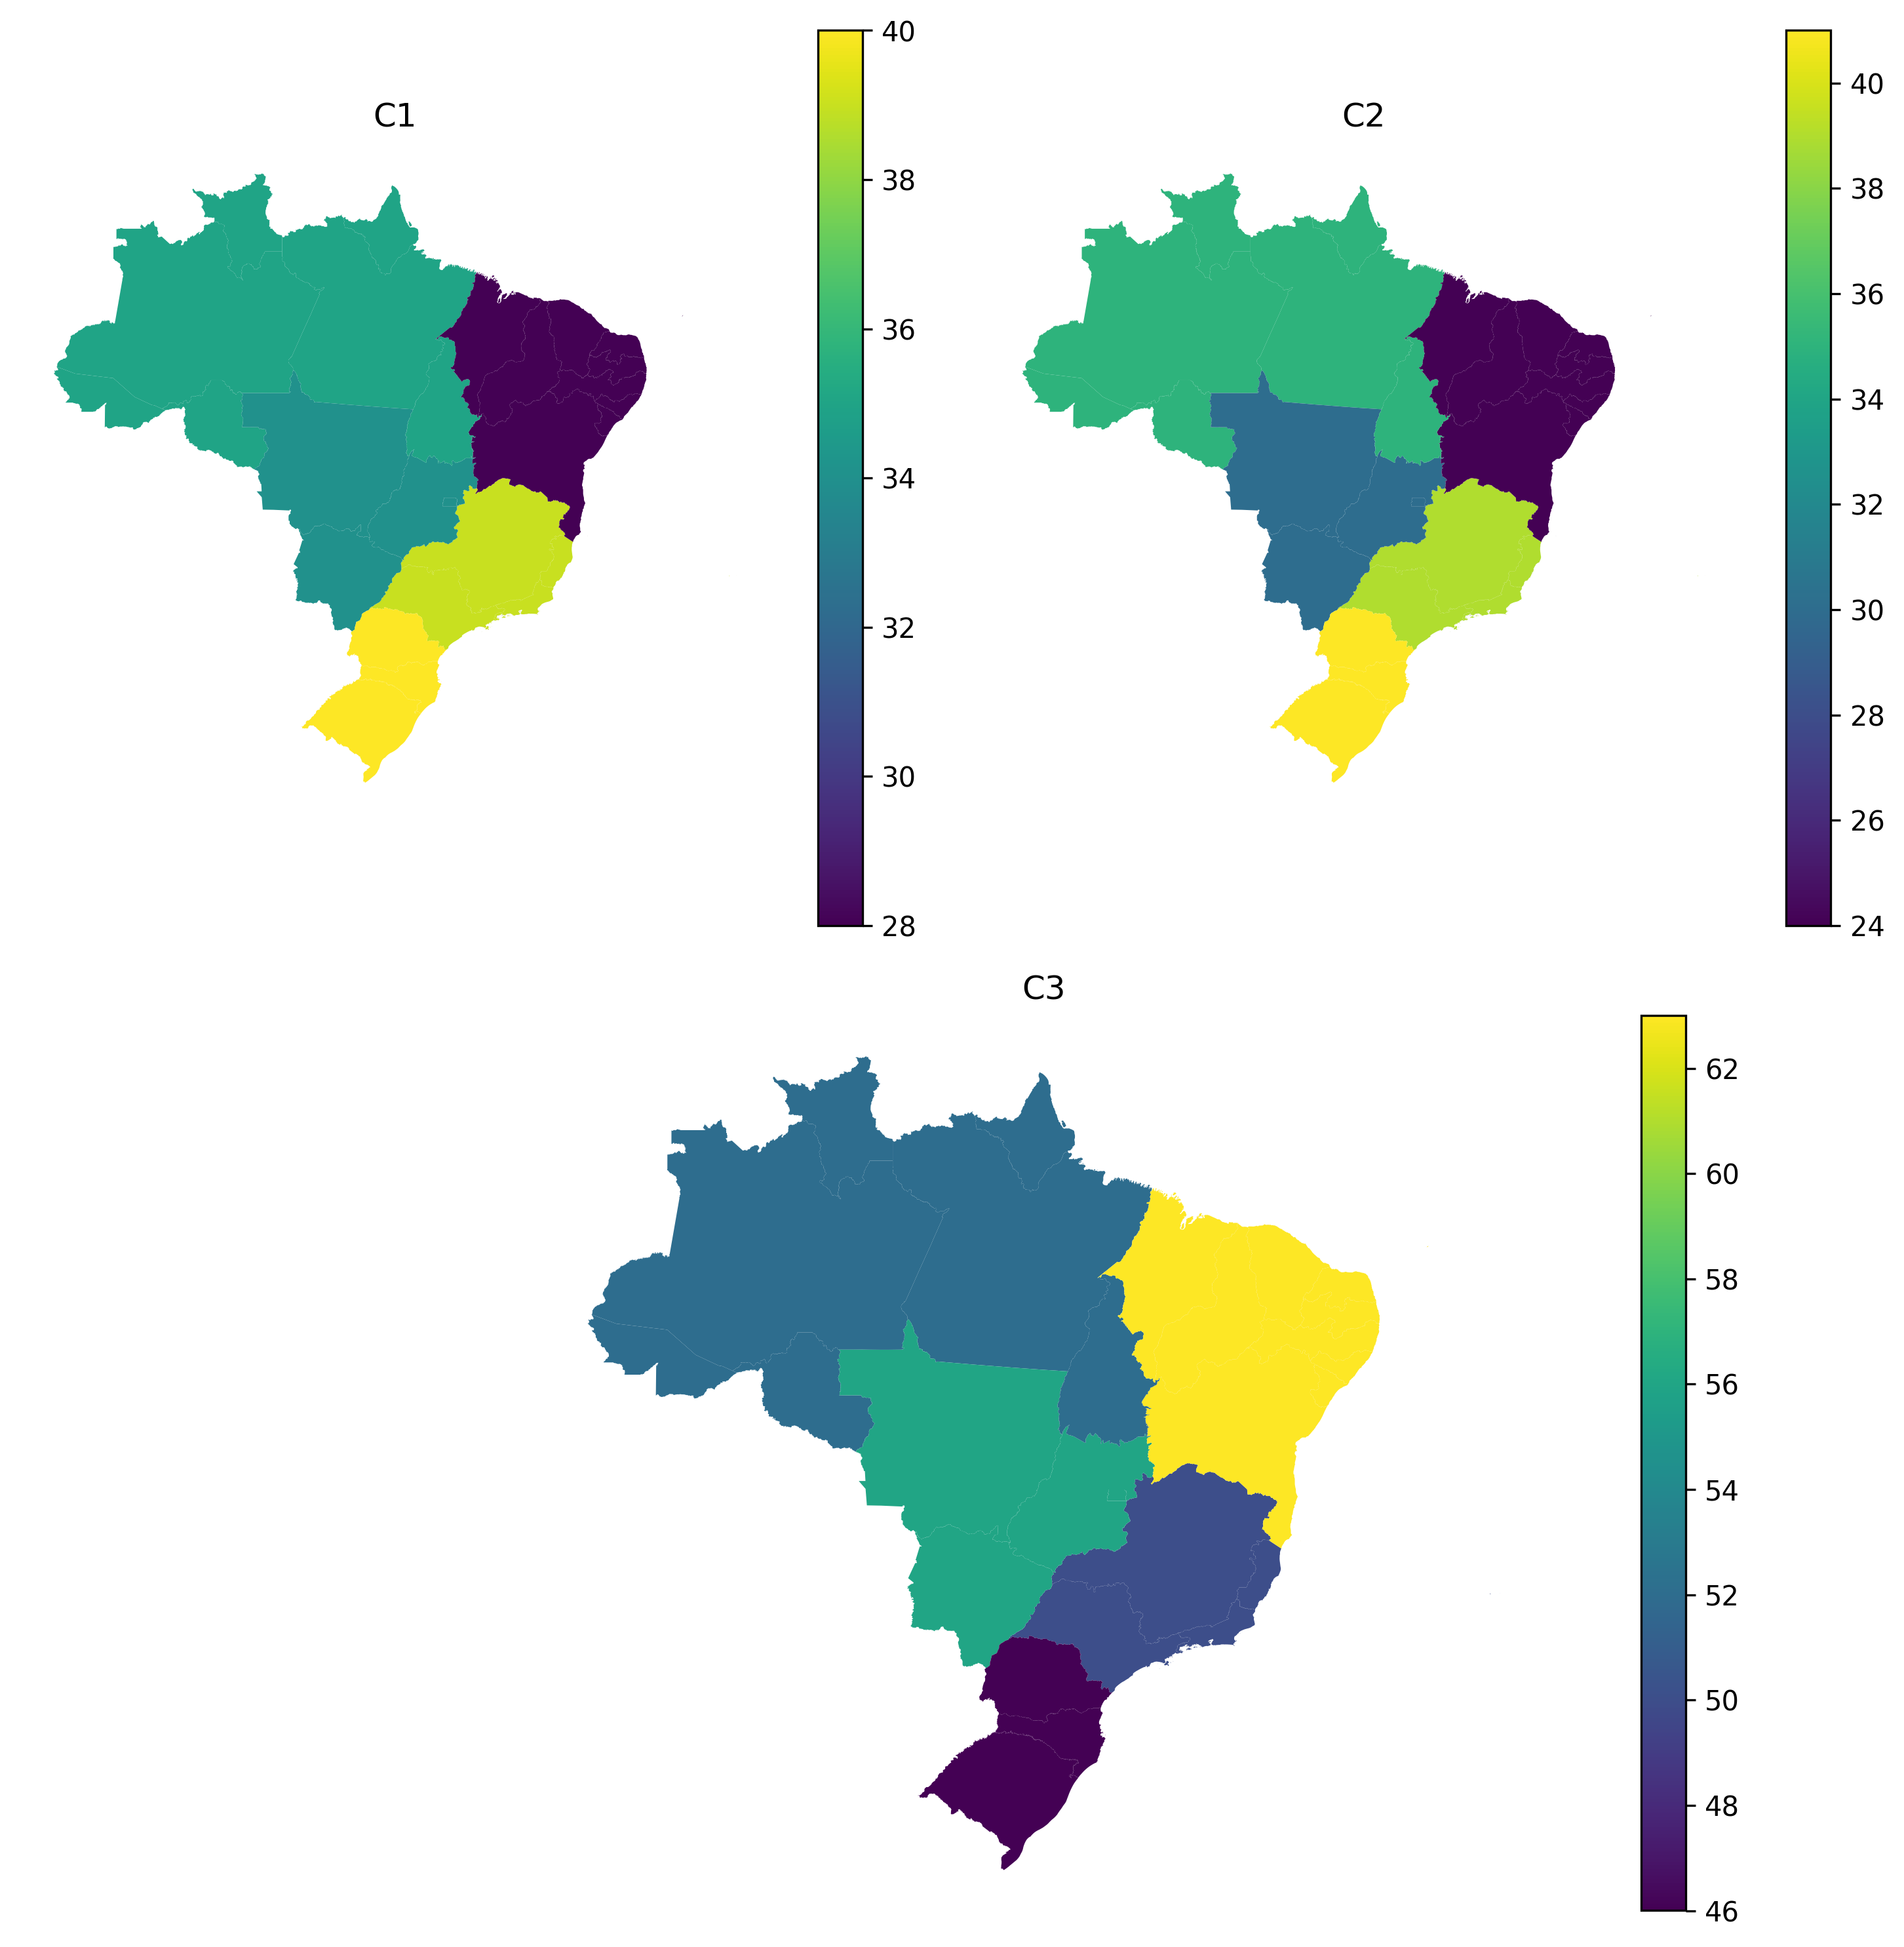
\includegraphics[width=1\linewidth]{figuras/mapa_coropletico_tic_domicilios_2024_g3.png}
	\label{fig:mapa_coropletico_tic_domicilios_2024_g3}
	\footnotesize{Fonte: elaboração própria baseade em \cite{tic_domicilios_2024_g3}.}
\end{figure}

No tocante ao critério G3-1, as regiões Sudeste e Sul foram as regiões em que mais houve procura de informações oferecidas pelo governo, seguidas do Centro-Oeste e Norte, e por fim, pelo Nordeste.

No tocante ao critério G3-2, a região Sul foi a região em que foram realizados alguns serviços públicos, como emitir documentos pela internet, preencher e enviar formulários online ou pagar taxas e impostos pela internet. A região que menos usou serviços públicos foi a Nordeste, superada pelas Centro-Oeste, Norte e Sudeste.

No tocante ao critério G3-3, o Nordeste foi a única região em que a internet não foi utilizada para interagir com as autoridades, seguido do Centro-Oeste e finalmente, o Sudeste e o Sul.

Como foi demonstrado por todas as figuras, nota-se como é notório o uso de governo eletrônico no Brasil. Tal resultado confirma a ideia de \cite{singh2007country}, que argumenta que o uso constante de governo eletrônico justifica sua existência, manutenção e evolução.

\section{Transação do governo eletrônico para o digital no Brasil}

Como expressado nos parágrafos anteriores, com as condições favoráveis, a transformação digital pode se tornar paupável, executável e planejável. Segundo \cite{mitkiewicz2024transformaccao}, a transformação digital pode ser entendida como o processo de utilização das tecnologias da informação e comunicação para gerar soluções visando resolver de forma inovadora e em larga escala os problemas do mundo.

De forma complementar, \cite{alenezi2022understanding} afirma que a transformação digital no governo ou no setor público refere-se ao engajamento diferente e inovador e o trabalho com as partes interessadas, desenvolvendo frameworks para os mecanismos de entrega de serviços eficientes e formação de novos relacionamentos.

No contexto dos parágrafos anteriores, surgem os governos digitais em substituição aos governos eletrônicos. \cite{veiga2016digital} afirma que, diferentemente do governo eletrônico, o governo digital não é apenas sobre tecnologia, é sobre uma operação multifacetada  que requer uma abordagem multidisciplinar e disciplina científica. 

\cite{bounabat2017government} complementa a ideia anterior. O auto cita que o governo digital baseia-se na divulgação aberta e sem precedentes de informações governamentais, aliada à troca em grande volume de informações altamente sensíveis e também pessoais entre agências governamentais e seus clientes. 

O governo digital traz diversos benefícios, além dos benefícios do governo eletrônico. \cite{martins2018war} argumenta que as ferramentas de governo digital promovem transparência, responsabilização e acesso melhorado à informação.

Outra vantagem é mencionada por \cite{veiga2016digital}. O autor afirma que o uso de governo digital e serviços públicos online têm um grande potencial de reduzir o fardo administrativo, bem como, promover inovação e crescimento econômico. Além de contribuir com a diminuição das atividades da economia informal, aumentando a quantidade de pessoas que pagam impostos e reduzindo a corrupção.

Para \cite{kreuz20184textordfeminine}, vive-se e assiste-se à chegada da 4ª Revolução Industrial, que imprime uma modificação substancial na forma pela qual as pessoas e os diversos sistemas se relacionam. 

Complementa \cite{kreuz20184textordfeminine} que o mundo jurídico e o poder estatal necessitam não apenas se adaptar, mas incorporar as tecnologias ao seu m\textit{modus operandi} como meio de implementar a participação social dos cidadãos no processo decisório. E assim, incorporar os preceitos reais de um constitucionalismo latino-americano.

\cite{kreuz20184textordfeminine} argumenta que o estudo de caso realizado mediante o Governo digital brasileiro fornece algumas respostas. O Brasil vem se adaptando e implementando as TICs nos seus processos de relação com a sociedade. A abertura de dados e transparência cresce a cada ano. 

\cite{kenosi2024industrial} em sua revisão da litaratura, indetificou que sua revião sistemática evidência que o potencial transformativo das tecnologias da Revolução Industrial 4.0 em melhorar os serviços de governo eletronico, focando na democrtização da administração pública vi a transparência melhorada, participação cidadã e entrega de serviços públicos.

No referido contexto, como marco legal da transição de governo eletrônico para digital  no Brasil, a \textbf{Lei do Governo Digital}, em seu artigo 1º, segundo \cite{l14129},  dispõe sobre princípios, regras e instrumentos para o aumento da eficiência da administração pública, especialmente por meio da desburocratização, da inovação, da transformação digital e da participação do cidadão.

\cite{carvalho2022nova} cita que Certamente, foi com a Lei nº 14.129, de 29 de março de 2021, que o maior passo foi dado no sentido de implantação do governo digital. A propósito, apesar de ter se autointitulado “lei do governo digital”, a citada legislação possui um campo de incidência ainda mais amplo.

Para \cite{carvalho2022nova}, no caso, o art. 1º da \textbf{Lei do Governo Digital} determina que a lei “dispõe sobre princípios, regras e instrumentos para o aumento da eficiência da administração pública”, e tal objetivo seria perseguido “especialmente por meio da desburocratização, da inovação, da  transformação digital e da participação do cidadão”. 

Para \cite{carvalho2022nova}, ademais, dentre os 26 princípios do governo digital e da eficiência pública (art. 3º), registre-se a presença tanto da “desburocratização, a modernização, o fortalecimento e a simplificação da relação do poder público com a sociedade, 
mediante serviços digitais”, como também do “incentivo à participação social no controle e na fiscalização da administração pública”.

Para \cite{carvalho2022nova}, a abertura de novos espaços de participação social na atividade administrativa do Estado trata-se de um importante passo para uma maior democratização da democracia, seja em relação ao aspecto quantitativo ou qualitativo, pois geralmente 
é a face da administração pública que apresenta o Estado ao cidadão.

\cite{carvalho2022nova} cita 4 aspectos do governo digital: 

\begin{itemize}
	\item Incremento da participação social pelo acesso dos 
cidadãos à informação e ao conhecimento
	\item A participação social digital gerando maior engajamento e 
empoderamento
	\item O governo digital aproximando a sociedade civil e o Estado
	\item Incremento da participação social viabilizada pelo monitoramento
\end{itemize}

Dos aspectos apresentados por \cite{carvalho2022nova}, será discutivo o aspecto do governo digital aproximando a sociedade civil e o Estado. Para \cite{carvalho2022nova}, um aspecto que precisa ser levado em consideração trata de uma forma de aproximação: a do Estado e da sociedade civil. Neste sentido, perceba-se que as novas tecnologias digitais não apenas permitem que a sociedade civil esteja informada, capacitada, engajada e empoderada. Elas também asseguram que o Estado possa melhor detectar qual são as aspirações dos cidadãos.

Complementarmente, para \cite{carvalho2022nova}, nesse momento de consolidação das redes sociais, vê-se a formação de uma opinião pública digital, que permite a qualquer cidadão expressar livremente suas opiniões e inclusive sugerir propostas de ação a serem adotadas pelo administrador público. O cidadão de hoje não pode apenas ser visto como um cliente da administração pública, mas sim um parceiro para a formulação e a execução de políticas estatais.

Para \cite{do2022governo}, a \text{Lei do Governo Digital}, propondo um modelo de governo digital que inaugure uma nova forma de relacionamento entre a Administração Pública e os destinatários de sua atuação, incorpora ferramentas de modificação na dinâmica tradicional regedora dessas mesmas relações.

Ainda para \cite{do2022governo}, em razão do argumento anterior, promove uma conciliação entre a racionalidade jurídica, que se encontra na regularidade do procedimento e na estabilidade das estruturas formais de organização e atuação, e a racionalidade da gestão, que tem por fonte de legitimidade a eficácia das ações desenvolvidas. 

\cite{do2022governo} elogia a mudança do paradigma legal introduzida pela \text{Lei do Governo Digital} como uma a iniciativa é de ser prestigiada, pois no alinhamento entre racionalidade jurídica e racionalidade da gestão tem-se a tradução de um direito fundamental à boa administração.

Porém, limitações para a implementação das políticas públicas de governo digital. \cite{reck2021transformaccao} cita que ainda falta muito a fazer, principalmente no que diz respeito ao processo de inclusão dos que não tem acesso aos serviços indispensáveis à busca de uma cidadania mais efetiva. 

\cite{reck2021transformaccao} complementa que o cenário do parágrafo anterior é composto por cerca de 30 milhões de pessoas, que não estão inseridos no processo democrático, em razão de não terem sido alcançados pelos serviços digitais.  Nos tempos atuais, as políticas públicas podem ser disseminadas por plataformas digitais, notadamente, pelo fato do avanço de serviços como o Governo Digital onde algumas ofertas estão cada mais exclusivas nesse meio, a citar o seguro-desemprego, meu SUS digital e previdência.

Assim, para  \cite{reck2021transformaccao}, vê-se que o exercício da cidadania para muitos, encontra obstáculos, faltando-lhes serem alcançados pelas TICs, bem como por uma educação voltada ao manejo da rede, como também, por lhes faltarem condições de acesso, especialmente à população mais vulnerável, como: negros, camponeses, ribeirinhos, povos originários, populações tradicionais, os de baixa renda; e os que mesmo tendo acesso, não tenham o necessário discernimento para fazê-lo com efetividade.

A \textbf{Lei do Governo Digital} nasceu do Projeto de Lei nº 7.843, de 2017. \cite{pl_lgd} cita como motivações para a proposição da inovação legislativa:

\begin{itemize}
    \item As críticas da qualidade ao atendimento do setor público.
    \item A precariedade e a falta de acesso a serviços públicos como fatores determinantes para o grave quadro de exclusão e desigualdade social que sempre marcou a sociedade brasileira. 
    \item  A simplificação das relações entre pessoas,
    sejam elas físicas ou jurídicas, com o poder público, tema essencial para o acesso a direitos básicos e, principalmente, para o desenvolvimento econômico.
    \item O excesso de exigências burocráticas, a baixa informatização, o ainda frágil acesso à informação, a falta de abertura das bases de dados públicos, a ausência de mecanismos de participação e inovação, além da corrupção, são alguns dos problemas que explicam a precariedade e ineficiência dos serviços públicos prestados
    nas três esferas da federação.
\end{itemize}

Nesse sentido, a \textbf{Lei do Governo Digital}, visando melhorar a administração pública, seu artigo 5º, conforme \cite{l14129}, serão utilizadas soluções digitais para a gestão de suas políticas finalísticas e administrativas e para o trâmite de processos administrativos eletrônicos.

Além disso, \textbf{Lei do Governo Digital}, segundo \cite{l14129}, determina sua aplicação às Administrações Direta e Indireta da União Federal e dos demais entes federados, desde que adotem os comandos da lei por meio de atos normativos próprios, vedada a aplicação da lei às empresas públicas e sociedades de economia mista, suas subsidiárias e controladas que não prestem serviço público.

Haja vista \cite{reck2021transformaccao}, o governo digital não se restringe à automação de processos e à disponibilização de serviços públicos on-line, busca avançar para um modelo de administração pública capaz de integrar as TICs a seus processos internos e aos cidadãos, buscando cumprir os papéis essenciais do Estado de forma mais eficiente, bem como restar serviços públicos mais qualificados. 

De forma complementar ao argumento anterior, \cite{lima2023governo}, com as inovações legislativas trazidas pela \textbf{Lei do Governo Digital}, especialmente com o enfoque em um modelo do Governo digital por plataforma, notadamente na esfera federal, a mudança está em sintonia com as mudanças tecnológicas, principalmente impulsionadas pela pandemia da Covid-19, guarda estrita sintonia com a ordem jurídica constitucional vigente e evidencia essa ordem de preocupação normativa da parte do Poder Público.

A maneira como o poder público se relaciona com a sociedade civil, sob a ótica do governo digital, segundo  \cite{lima2023governo}, é via as plataformas de governo digital, pois constituem realizações que buscam a aproximação entre Administração e cidadãos e cidadãs na esfera digital e, adicionalmente, são os meios pelos quais a atuação pública alcança suas finalidades.

Para \cite{de2020governo}, ao longo dos anos, a administração pública no Brasil se estruturou e foi moldada a partir de um amálgama entre uma concepção jurídica formalista, práticas burocráticas e uma generalizada cultura da desconfiança. 

\cite{de2020governo} complementa a ideia anterior citando as diversas faces 
conhecidas do modelo democrático:  

\begin{itemize}
    \item Interpretações e decisões baseadas em conceitos abstratos, ignorando as suas consequências práticas, defesa de ritos e formas como um fim em si mesmo, exigências de regularização desnecessárias.
    \item Um ambiente institucional que incentiva e premia o conservadorismo e a apatia de servidores e gestores públicos.
\end{itemize}

\cite{de2020governo} argumenta que as iniciativas de governo digital - sucessoras do governo eletrônico - pretendem, justamente, transformar a realidade do modelo burocrático inefetivo, eficaz  e ineficiente, mediante a instituição de serviços públicos digitais, que sejam mais simples, céleres e eficientes.

A implementação das iniciativas de governo digital trata-se, segundo \cite{de2020governo}, da construção de um novo paradigma  de administração pública, fundado sobre os princípios da transparência, da inovação e da confiança  segundo os quais o uso das tecnologias digitais pode e deve viabilizar: 

\begin{itemize}
    \item A ampliação do acesso às informações públicas e a simplificação de 
    mecanismos de prestação de contas e de interação entre a administração 
    pública e a sociedade, incluindo a instituição de novos mecanismos de 
    avaliação dos serviços.
    \item A efetiva e constante inovação, mediante a adoção de modelos 
    administrativos e jurídicos flexíveis, a admissibilidade controlada do risco, a relativa tolerância ao erro, o questionamento de práticas vigentes e a criação de incentivos para a experimentação e para a implementação de soluções criativas por parte de gestores públicos.
    \item Com base na arquitetura disponibilizada pelas tecnologias digitais, a constituição de novos modos de produção da confiança, por meio dos quais seja possível a redução de exigências burocráticas, bem como a garantia de maior simplicidade, celeridade, previsibilidade e segurança nas relações entre cidadãos e órgãos e entidades públicos.
\end{itemize}

Relativo ao primeiro tópico, o Brasil sanou o problema citado com a aprovação da Lei nº 12.527, de 2011 - Lei de Acesso à Informação e com a implementação dos portais da transparência do órgãos e Poderes dos Entes Federados.

O segundo tópico foi sanado pelo \textbf{Lei do Governo Digital} pela criação dos laboratórios de inovação. Para \cite{l14129}, laboratório de inovação é um espaço aberto à participação e à colaboração da sociedade para o desenvolvimento de ideias, de ferramentas e de métodos inovadores para a gestão pública, a prestação de serviços públicos e a participação do cidadão no exercício do controle sobre a administração pública.

O último e terceiro tópico foi sanado com a determinação legal de que apenas o CPF, para pessoas físicas, e o CNPJ, para pessoas jurídicas, como a única forma de identificação aceita pela administração pública, haja vista a \textbf{Lei do Governo Digital} (art. 28, \textbf{caput}), conforme exposto por \cite{l14129}: "Art. 28.  Fica estabelecido o número de inscrição no Cadastro de Pessoas Físicas (CPF) ou no Cadastro Nacional da Pessoa Jurídica (CNPJ) como número suficiente para identificação do cidadão ou da pessoa jurídica, conforme o caso, nos bancos de dados de serviços públicos, garantida a gratuidade da inscrição e das alterações nesses cadastros."

Independentemente dos benefícios apresentados pelos argumentos anteriores, considerando \cite{de2020governo} a ideia de que há diversos obstáculos que podem dificultar ou desvirtuar o sentido e os resultados das políticas de governo digital, dentre elas: o risco de digitalização de fachada e se foi realizada sem as devidas salvaguardas técnicas e jurídicas.

No tocante ao risco de digitalização de fachada, segundo \cite{de2020governo}, pode ocorrer a manutenção da lógica burocrática tradicional sob uma roupagem eletrônica, equívoco muitas vezes encontrado na administração pública brasileira. O segundo problema, a incorporação de tecnologias digitais pode gerar externalidades negativas, produzindo novos riscos e incertezas ou, ainda, abusos e violação de direitos.

Outros fatores são citados como barreiras para a implementação das políticas de governo digital, são para \cite{do2022governo}: 

\begin{itemize}
    \item No campo da resistência cultural, o investimento, obrigatoria
    mente, deve ser no treinamento e na formação das lideranças públicas 
    a conduzirem o processo.
    \item Na relação com o controle, as iniciativas associadas 
    ao governo digital devem se pautar, principalmente, pelo sempre pres
    tigiado vetor da transparência
\end{itemize}

No tocante ao primeiro tópico, \cite{do2022governo} afirma que o investimento, obrigatoriamente, deve ser no treinamento e na formação das lideranças públicas 
a conduzirem o processo. Educação digital deve ser a palavra de ordem dentro da Administração, para os seus próprios agentes, e em favor dos destinatários do governo digital. 

Como resultado da educação para mitigar a resistência à digitalização do poder público, segundo \cite{do2022governo}, ampliada a educação digital, o valor inerente ao governo de mesmo cariz resta autoevidente, e com isso a tendência é de mitigação da resistência a partir da perspectiva de constrição fiscal.

No tocante ao segundo e último tópico, \cite{do2022governo} argumenta que na relação com o controle, principalmente, pelo sempre prestigiado vetor da transparência. O problema não está em navegar em mares nunca dantes navegados, mas sim, em não ter clareza quanto às ondas que se possam ter pela frente.
\chapter{Digitalização das áreas-meio e fim do Poder Judiciário}

Esta capítulo discutirá a digitalização das áreas-meio e fim do Poder Judiciário, focando no Sistema Eletrônico de Informação (SEI), Creta, Plataforma Digital do Poder Judiciário Brasileiro (PDPJ-Br) e o  Processo Judicial Eletrônico (PJe).

\section{Poder Judiciário na redemocratização}

O Brasil pós-democrático foi implementado como uma república  federativa, em concordância com \cite{cf88}, formada pela união indissolúvel dos Estados e Municípios e do Distrito Federal, constitui-se em Estado Democrático de Direito, cujos Poderes são o Executivo, Legislativo e Judiciário.

Haja vista o foco deste trabalho é o Poder Judiciário, esse Poder é composto, segundo \cite{cf88}, no art. 92 da Constituição Federal:

\begin{itemize}
    \item Supremo Tribunal Federal.
    \item Conselho Nacional de Justiça.
    \item Superior Tribunal de Justiça.
    \item Tribunais Regionais Federais e Juízes Federais.
    \item Tribunais e Juízes do Trabalho.
    \item Tribunais e Juízes Eleitorais.
    \item Tribunais e Juízes Militares.
    \item  Tribunais e Juízes dos Estados e do Distrito Federal e Territórios.
\end{itemize}

\cite{cf88} concedeu ao Poder Judiciário autonomia administrativa e financeira. A importância da autonomia para o Poder Judiciário se confirma ao analisar as figuras seguintes relativas ao controle judicial sob o Poder Executivo,  corrupção no Poder Judiciário, Estado de Direito e a corrupção política.

A figura \ref{fig:judicial-constraints-on-the-executive-index} mostra a situação mundial do controle judicial sobre o Poder Executivo em 2024.

\begin{figure}[H]
	\centering
	\caption{Índice de controle judicial sobre o Poder Executivo}
	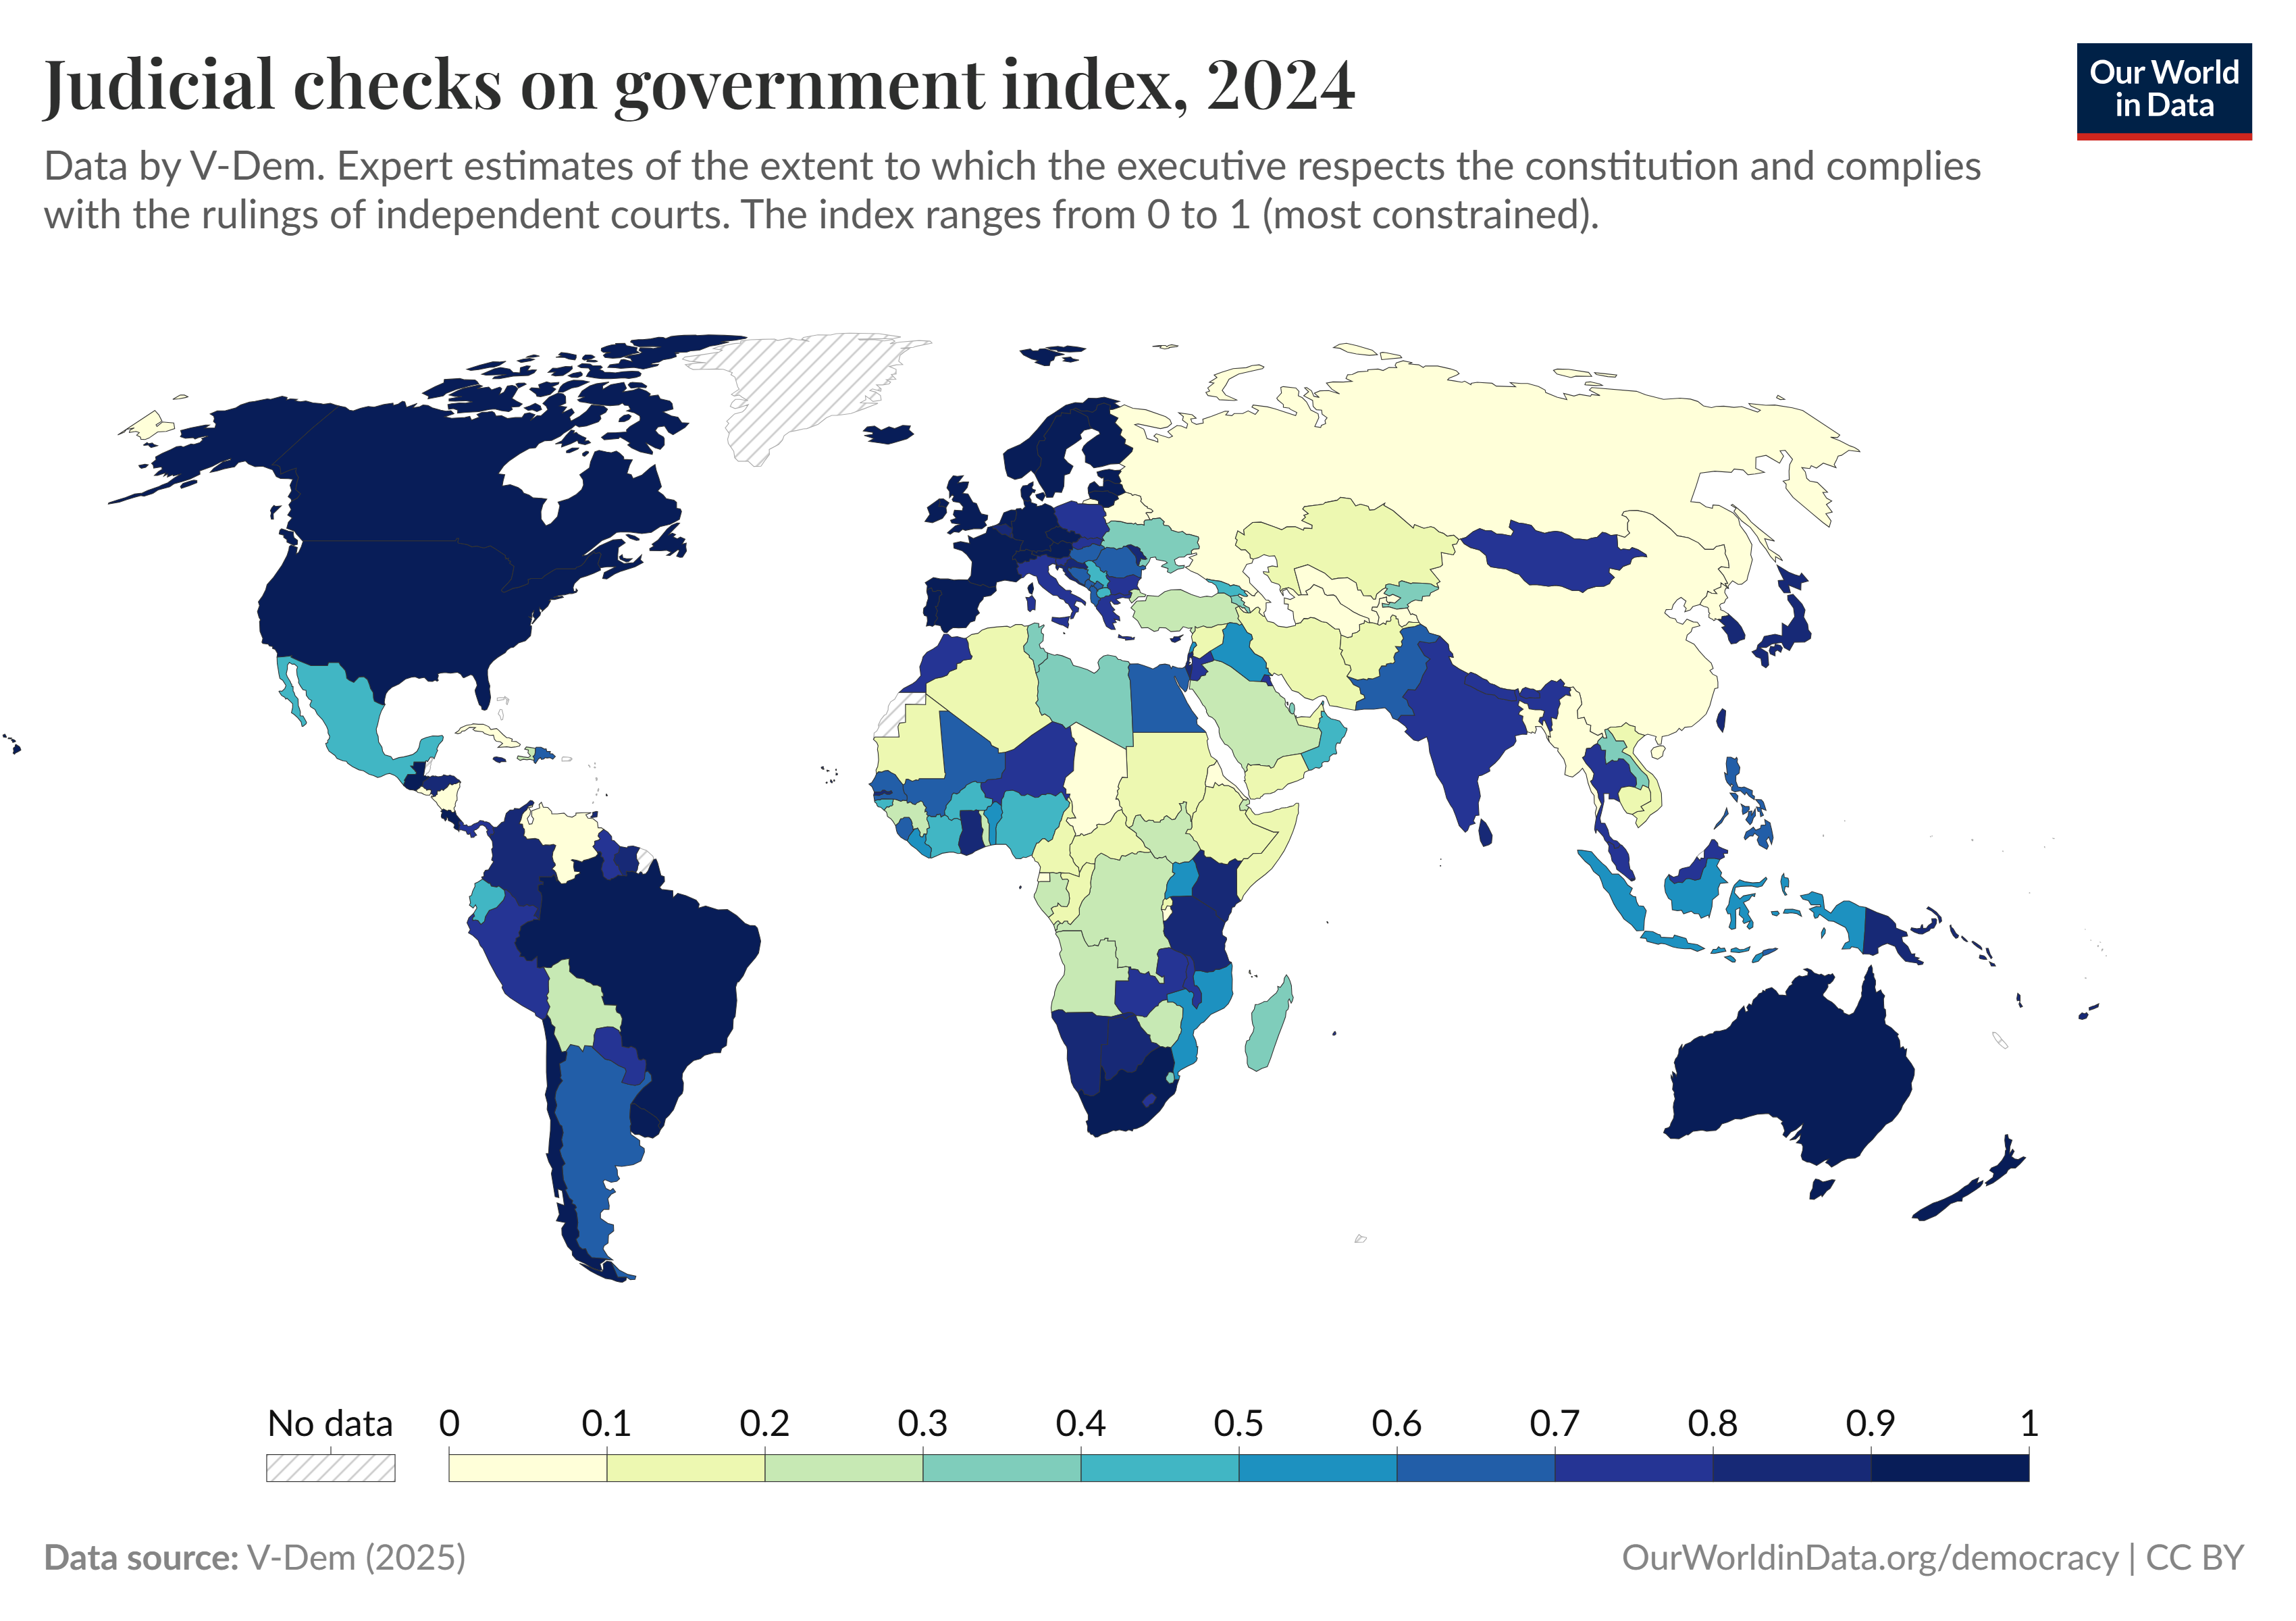
\includegraphics[width=1\linewidth]{figuras/judicial-constraints-on-the-executive-index.png}
	\label{fig:judicial-constraints-on-the-executive-index}
	\footnotesize{Fonte: \cite{jus_constraints_on_gov}.}
\end{figure}

Nota-se como o Poder Judiciário tem pouquíssimo controle sobre o Poder Executivo na em uma quantidade grande de países. A figura detalha o referido controle judicial no Brasil desde 1822 até 2024.

\begin{figure}[H]
    \centering
    \caption{Índice de controle judicial sobre o Poder Executivo no Brasil (1822-2024)}
    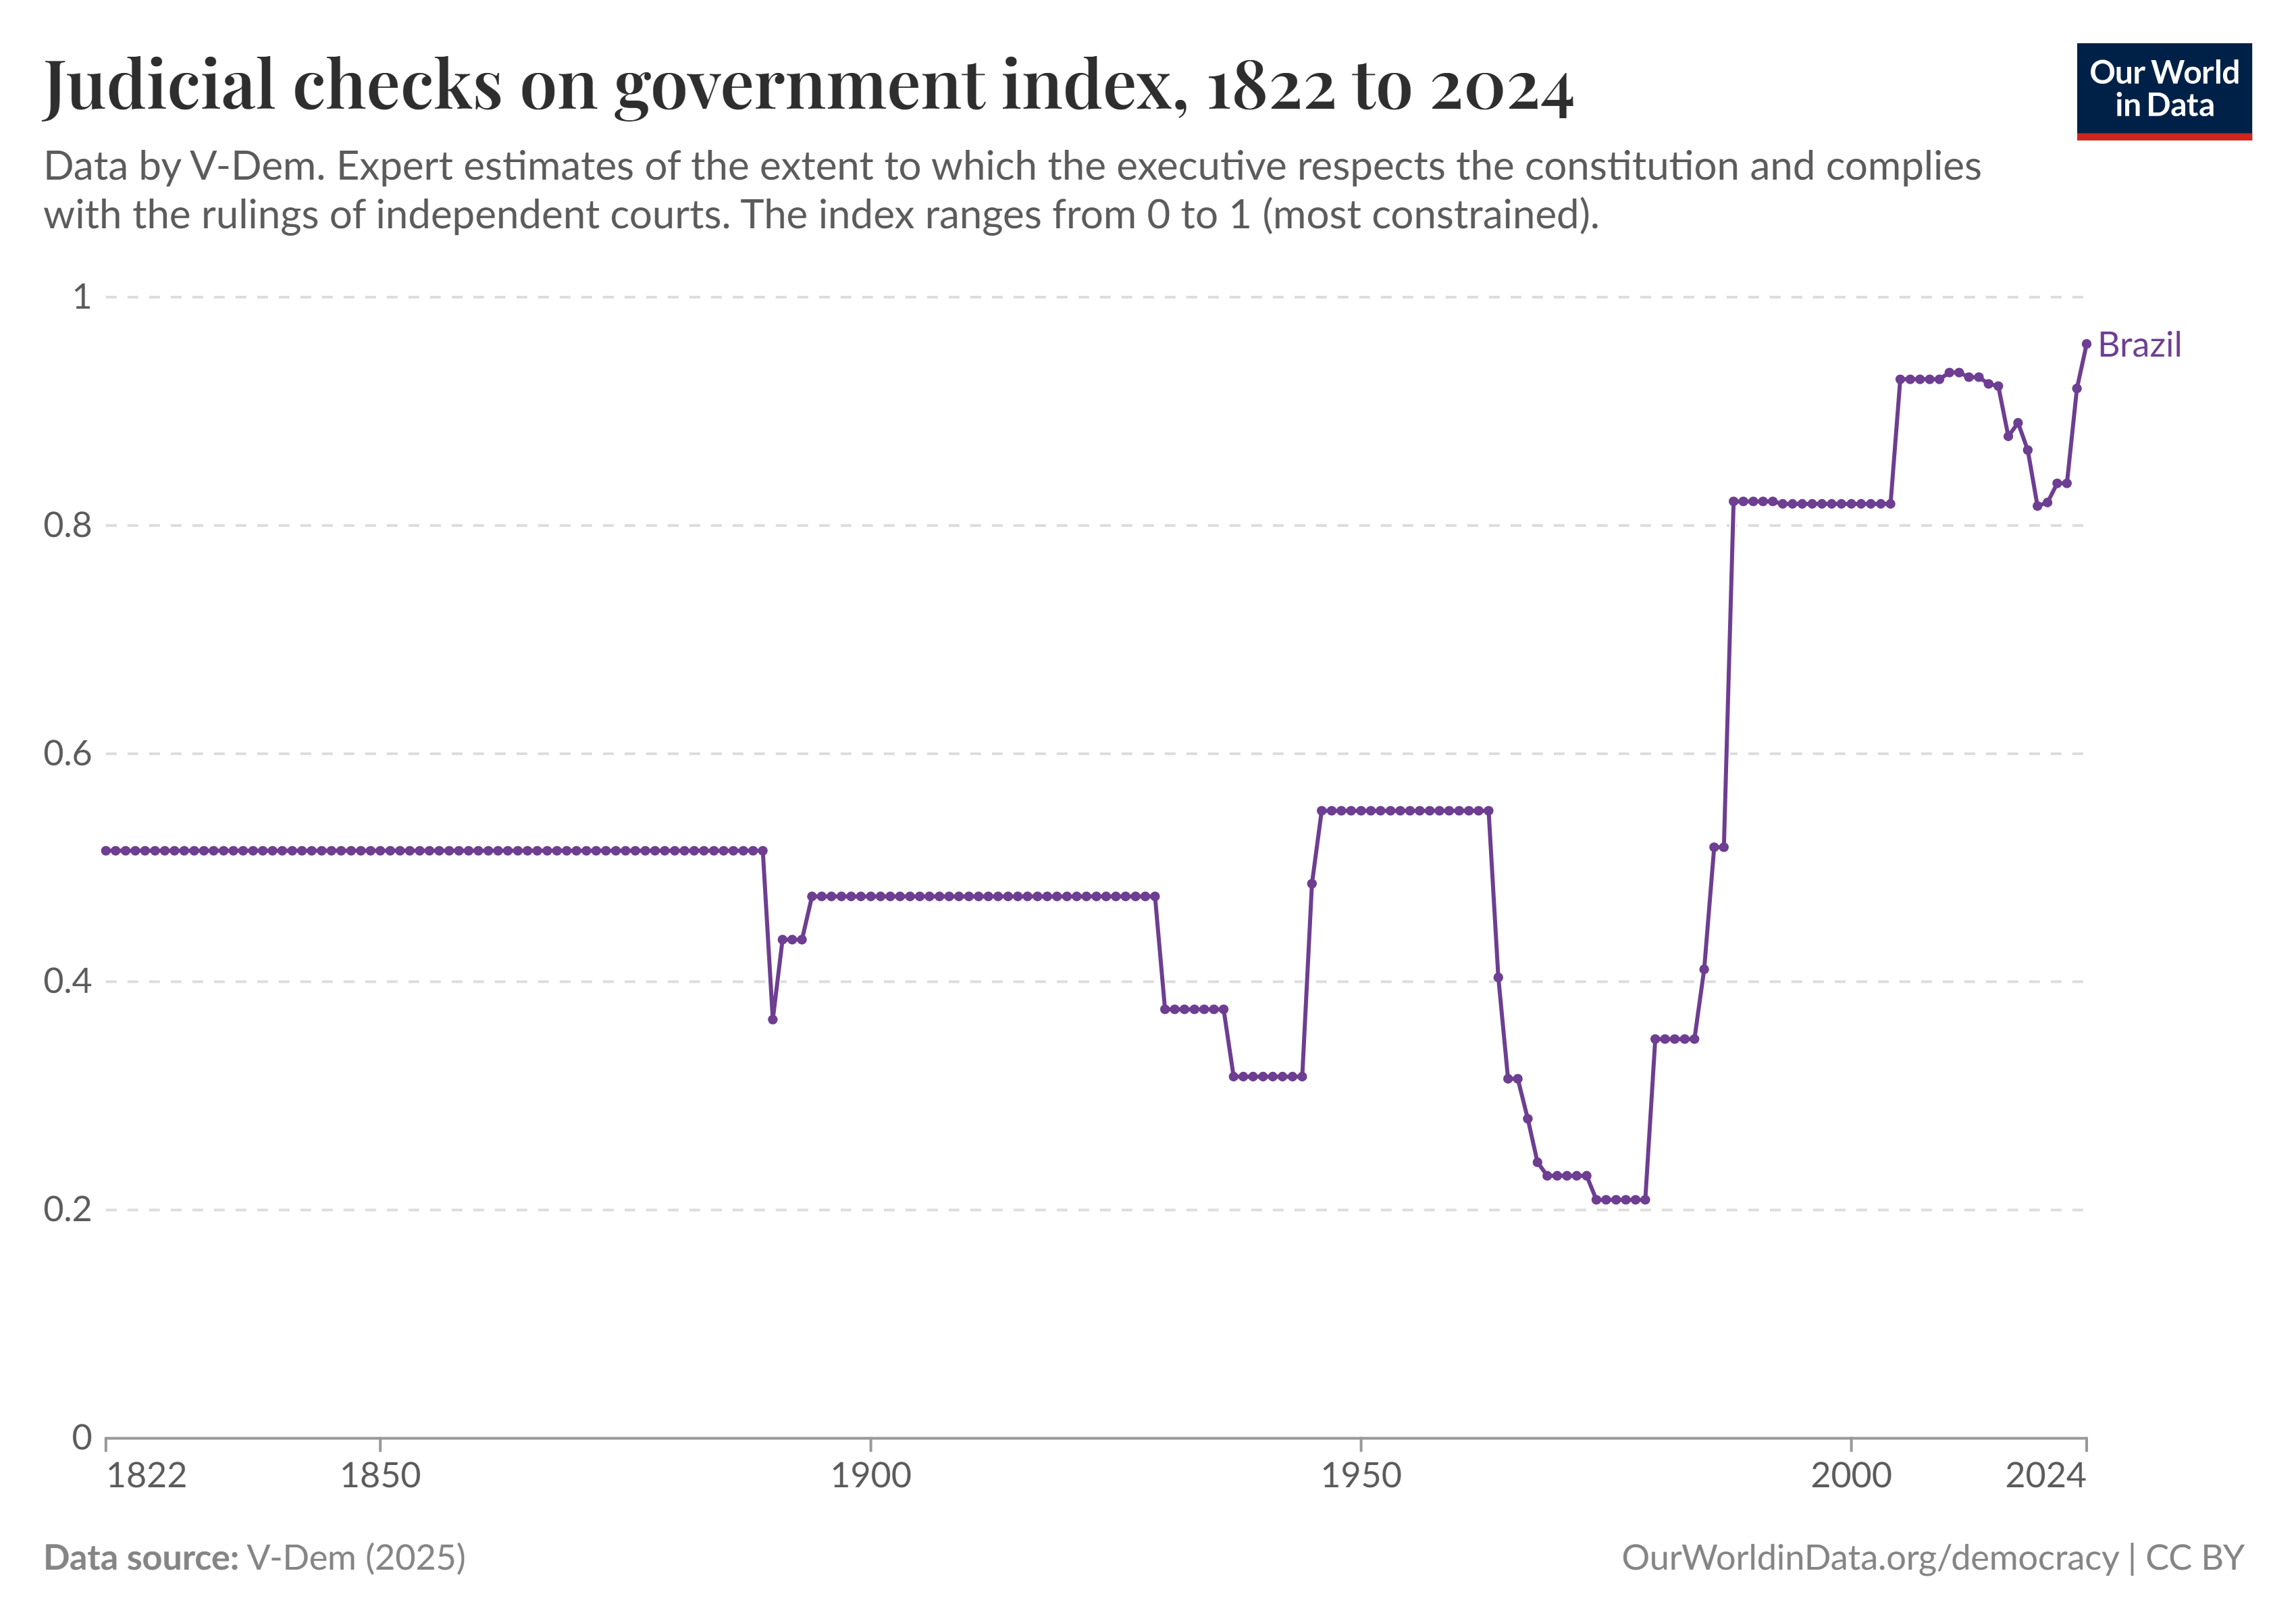
\includegraphics[width=1\linewidth]{figuras/judicial-constraints-on-the-executive-index-brazil.png}
    \label{fig:judicial-constraints-on-the-executive-index-brazil}
    \footnotesize{Fonte: \cite{jus_constraints_on_gov}.}
\end{figure}

No tocante a figura \ref{fig:judicial-constraints-on-the-executive-index-brazil}, nota-se como a democracia melhorou os índices do Brasil. Em 2024, o Brasil quase atingiu o valor máximo - 0,96 - enquanto a média mundial foi 0,664. Apenas 31 países de 193 - equivalente a 16\% do total - alcançaram uma pontuação de, no mínimo, 0,9 de 1,0 até o máximo.

A figura \ref{fig:quartis_controle_jus_sobre_gov} contém o Índice de controle judicial sobre o Poder Executivo.

\begin{figure}[H]
    \centering
    \caption{Índice de controle judicial sobre o Poder Executivo}
    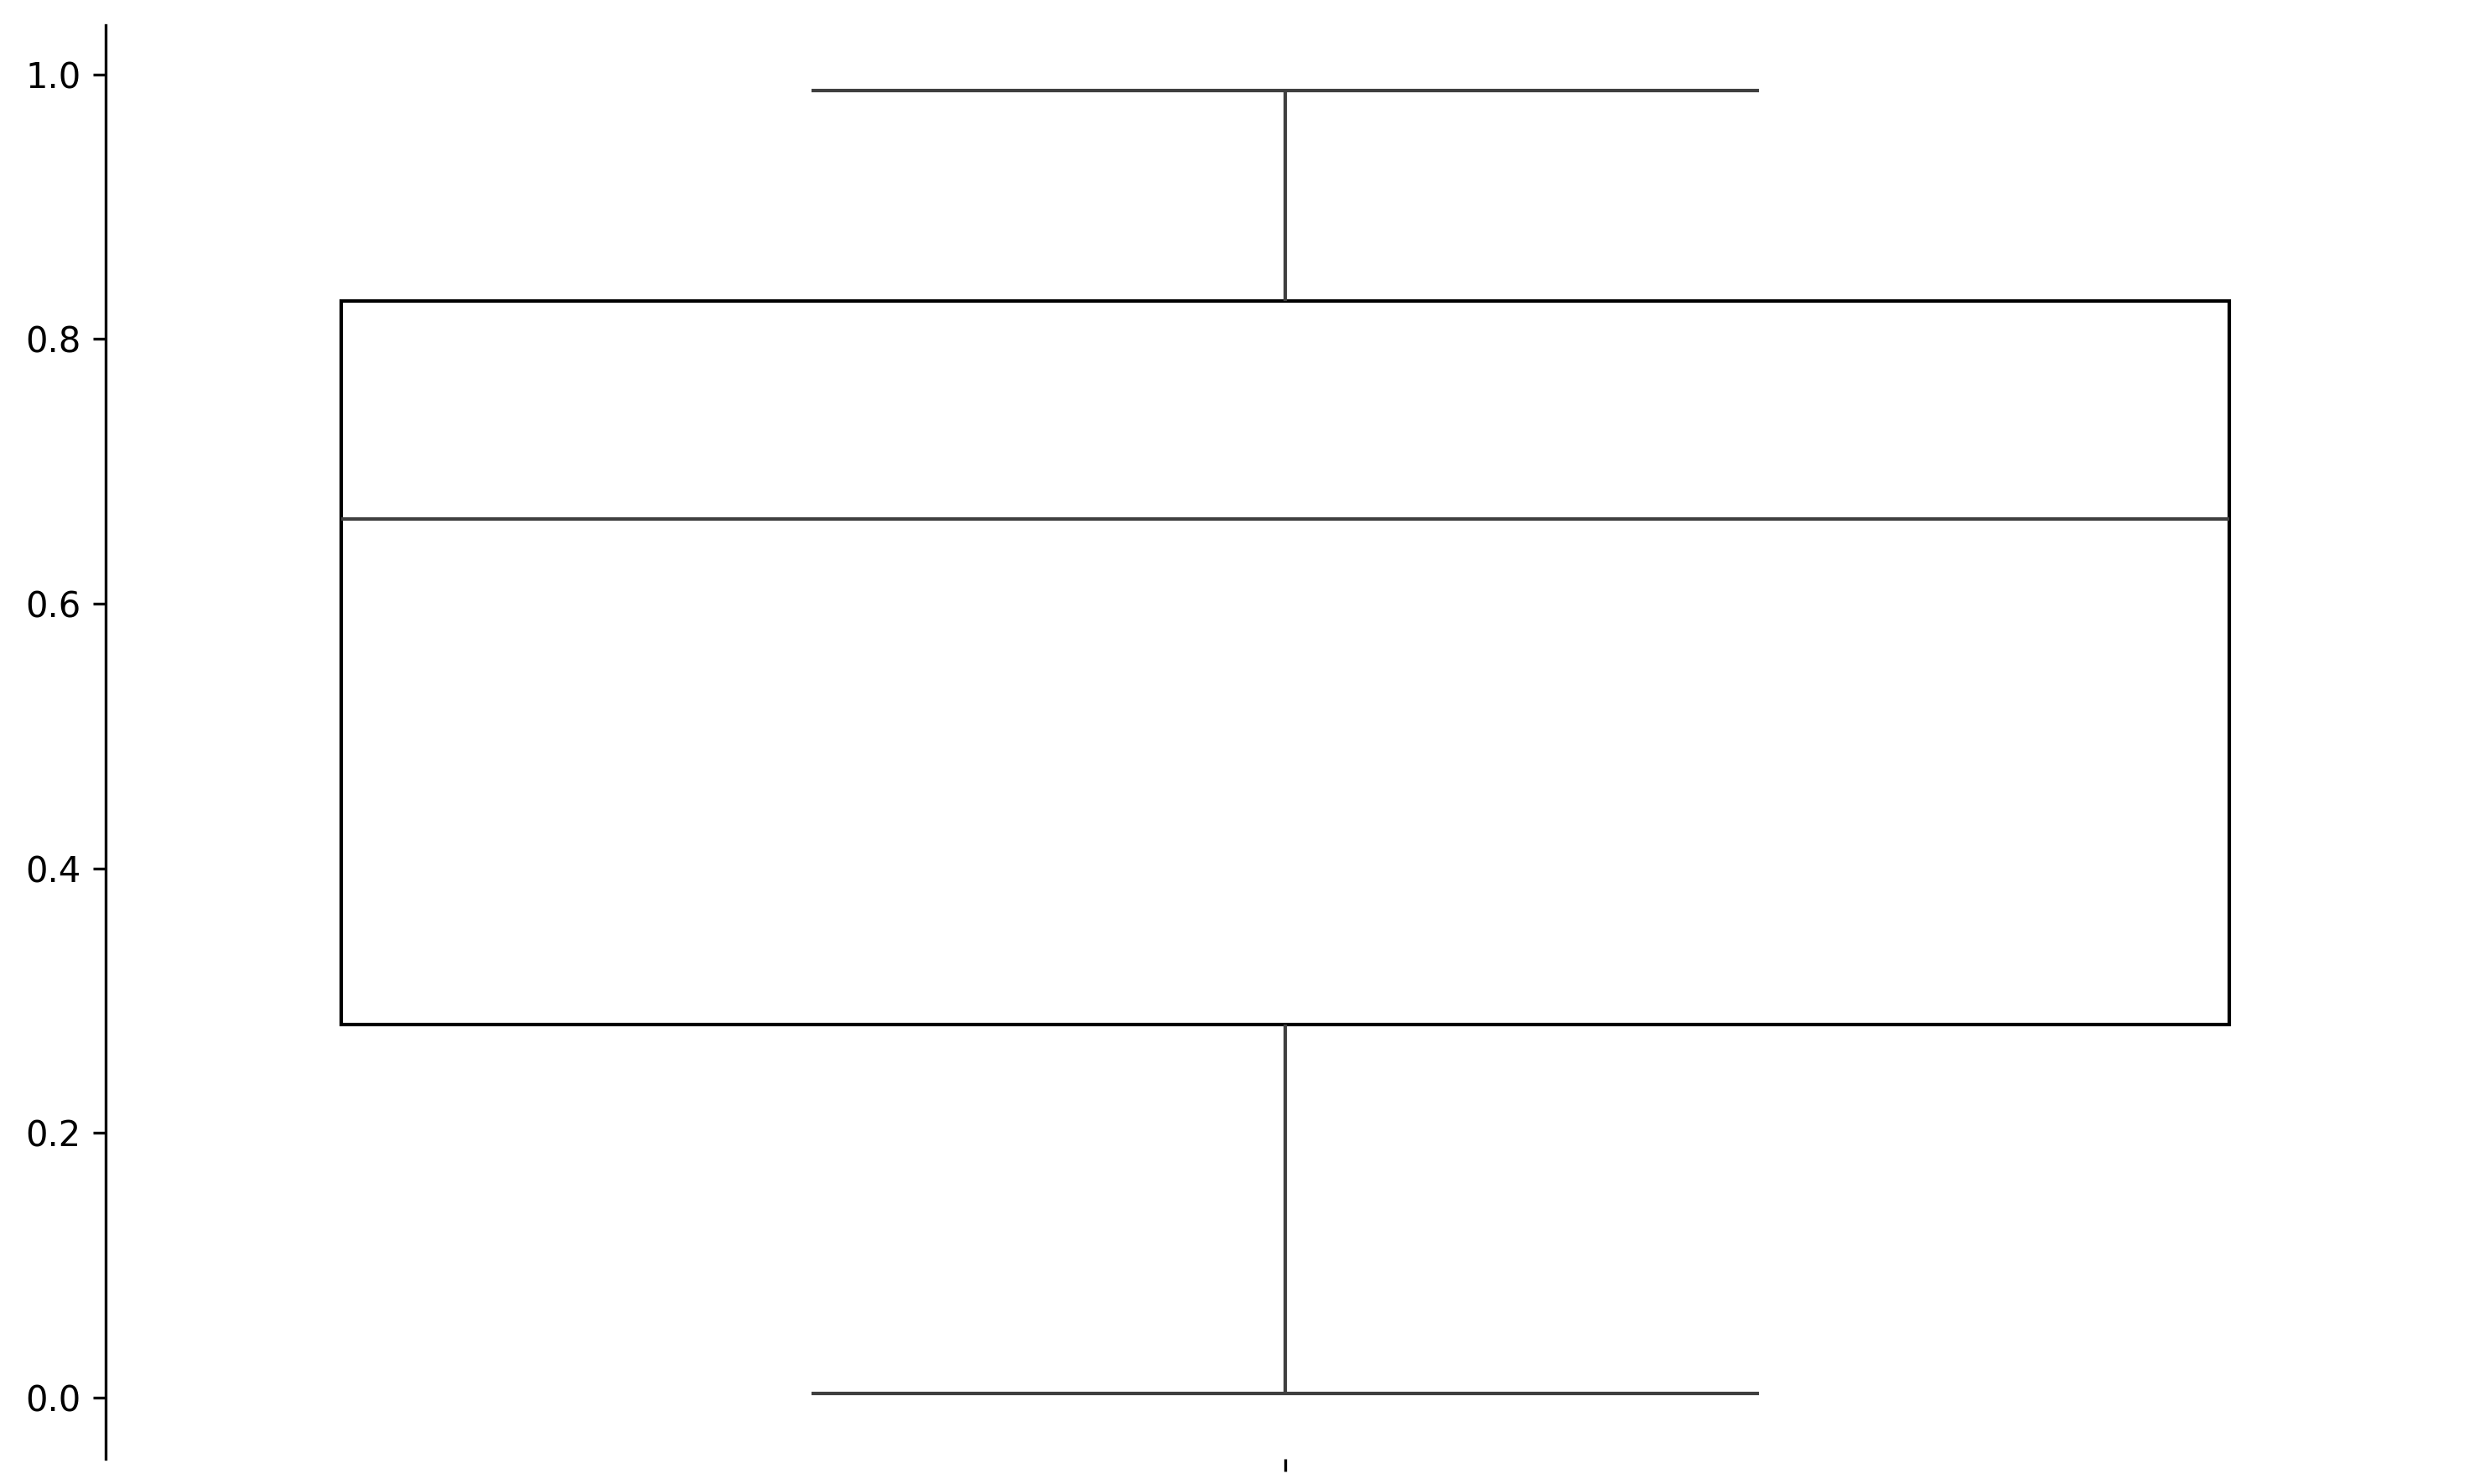
\includegraphics[width=1\linewidth]{figuras/quartis_controle_jus_sobre_gov.png}
    \label{fig:quartis_controle_jus_sobre_gov}
    \footnotesize{Fonte: elaboração própia baseada em \cite{jus_constraints_on_gov}.}
\end{figure}

A figura \ref{fig:quartis_controle_jus_sobre_gov}, que mostra a distribuição do índice de controle judicial sobre o Poder Executivo, ilustra que no ano de 2024 teve um valor mínimo de 0,003 e um máximo de 0,988. A média dos dados foi de 0,664. Além disso, 25\% dos valores ficaram abaixo de 0,282 (1º quartil), enquanto 75\% dos valores foram inferiores a 0,829 (3º quartil).

A figura \ref{fig:judicial-corruption-score} mostra os índices globais de corrupção judiciária.

\begin{figure}[H]
	\centering
	\caption{Pontuação de corrupção judicial no mundo em 2024}
	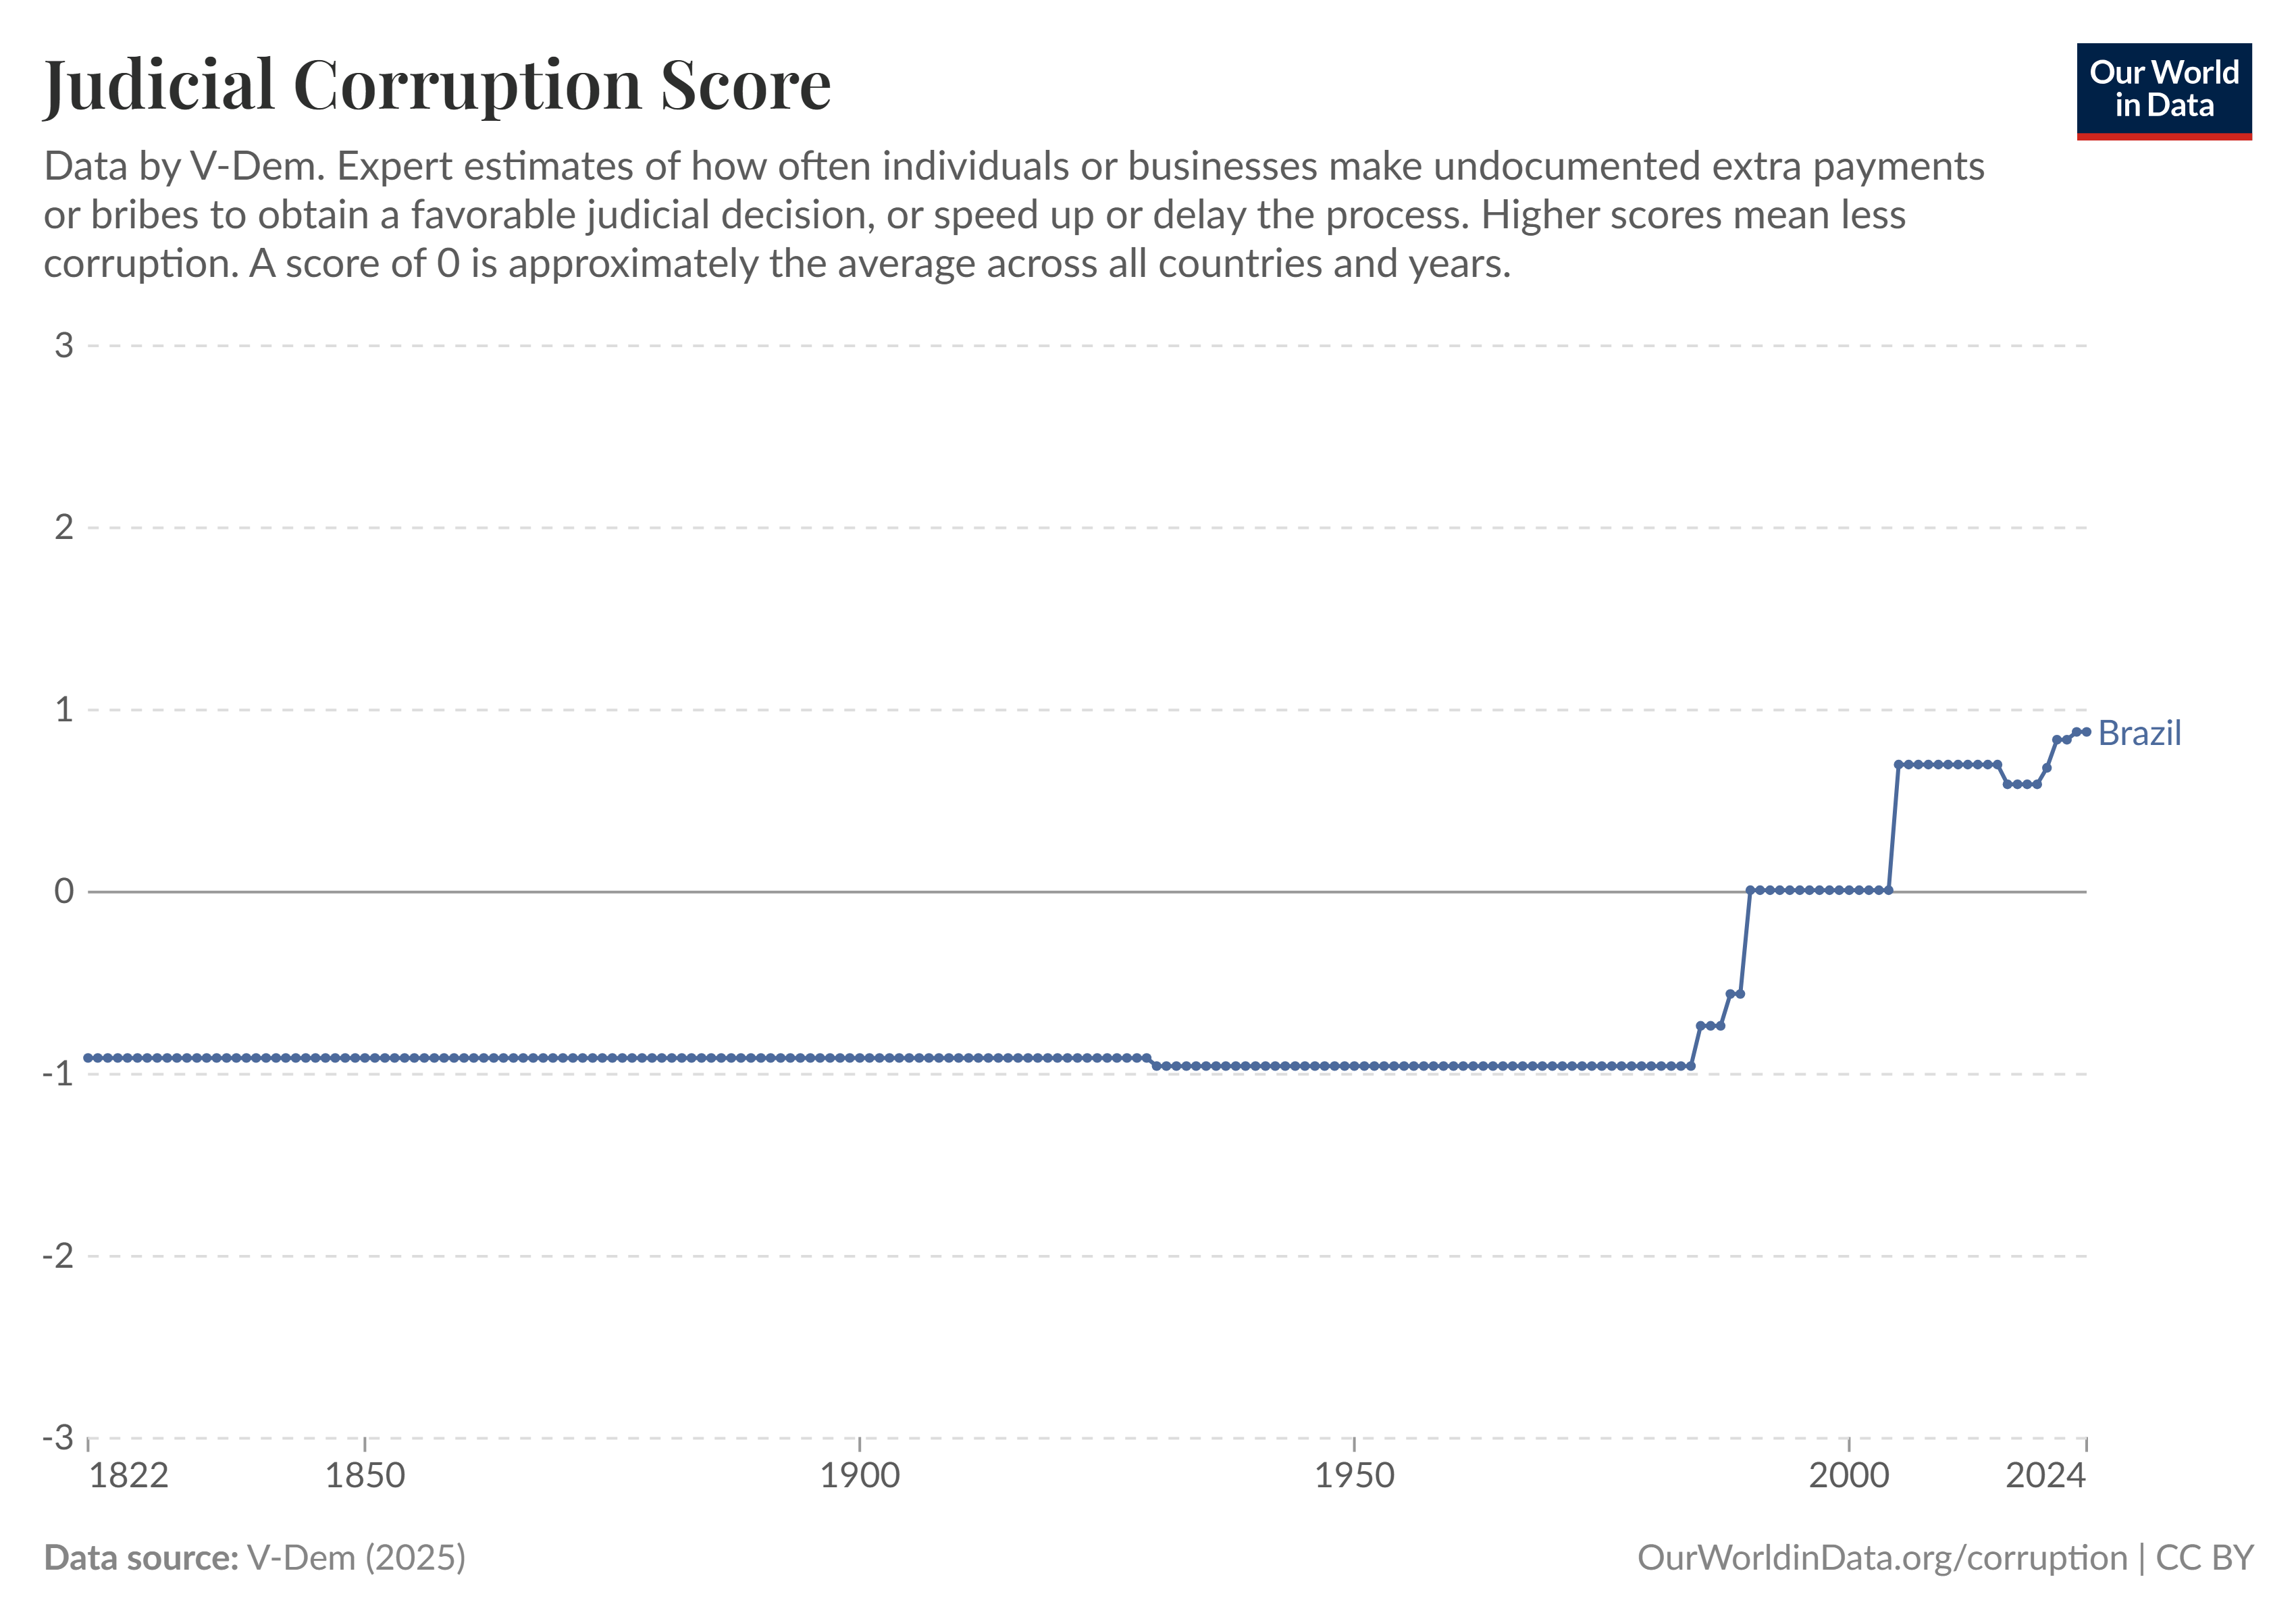
\includegraphics[width=1\linewidth]{figuras/judicial-corruption-score.png}
	\label{fig:judicial-corruption-score}
	\footnotesize{Fonte: \cite{judicial-corruption-score}.}
\end{figure}

Nota-se que uma quantidade grande de países tem alta corrupção judiciária. A figura \ref{fig:judicial-corruption-score} complementa a anterior ao especificar a situação histórica do Brasil (desde 1822 até 2024).

A figura \ref{fig:judicial-corruption-score-brazil} mostra como o Brasil melhorou o aspecto da corrupção judiciária. 

\begin{figure}[H]
    \centering
    \caption{Pontuação de corrupção judicial no Brasil (1822-2024)}
    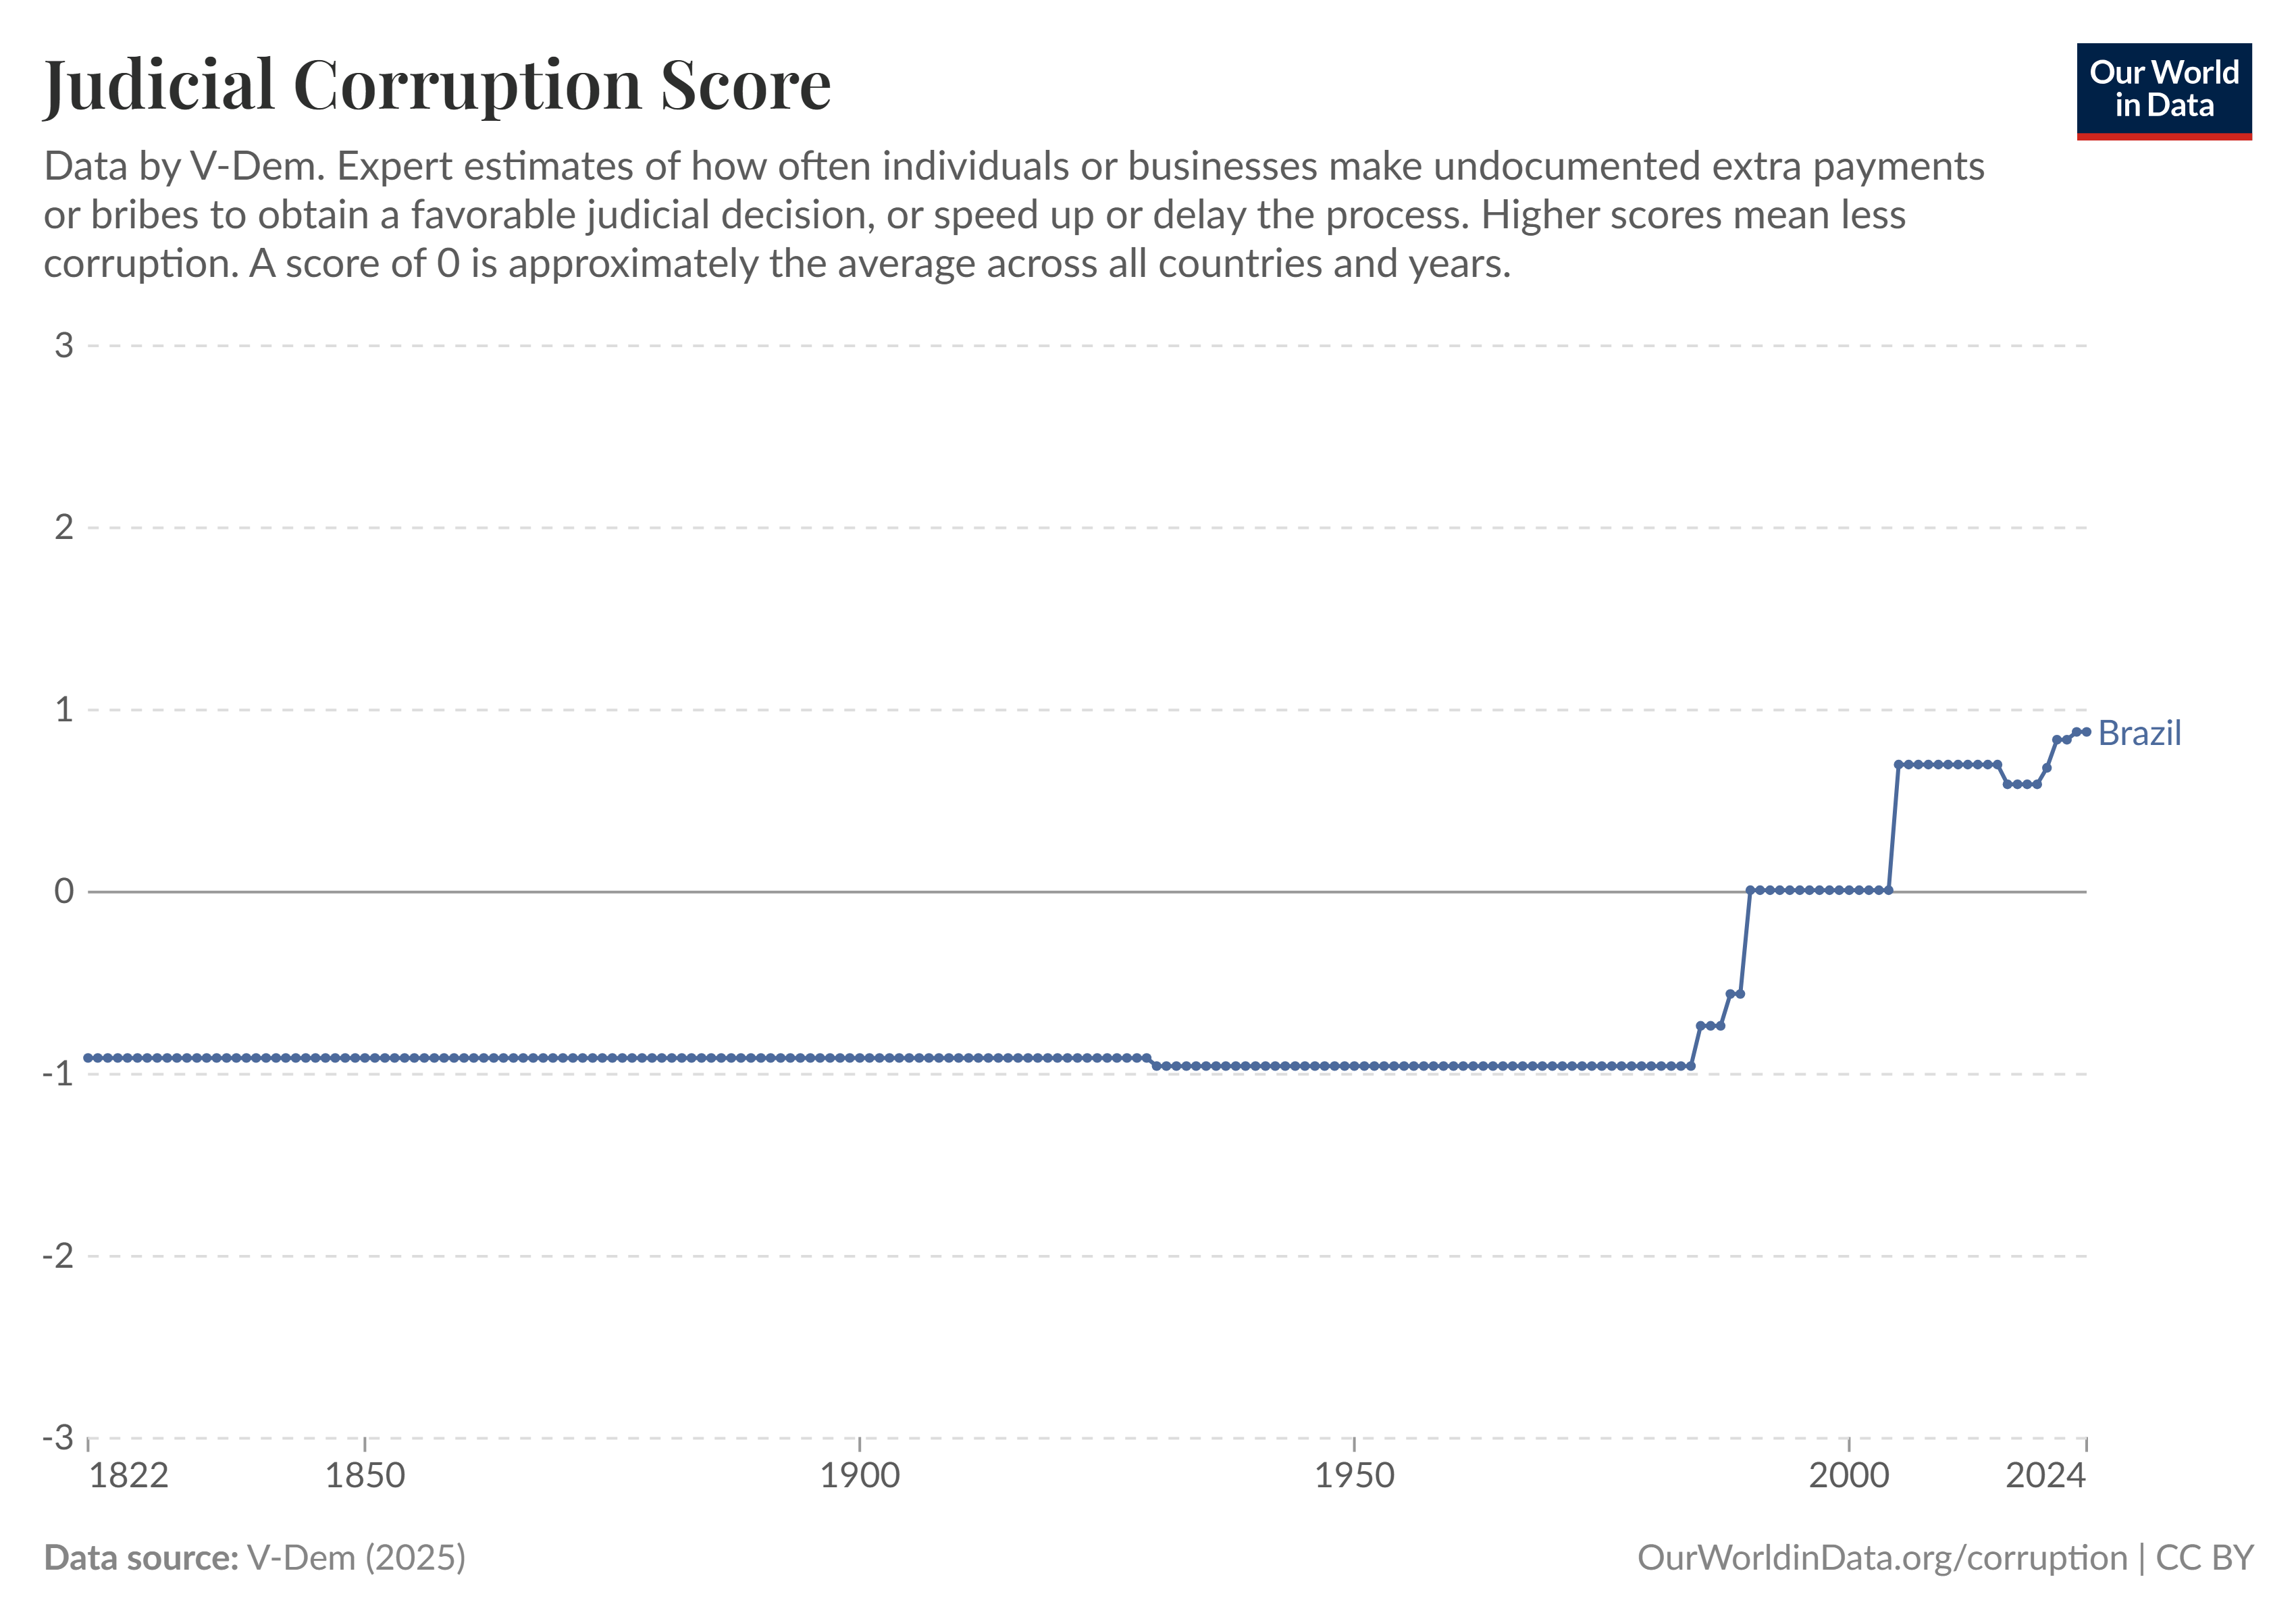
\includegraphics[width=1\linewidth]{figuras/judicial-corruption-score-brazil.png}
    \label{fig:judicial-corruption-score-brazil}
    \footnotesize{Fonte: \cite{judicial-corruption-score}.}
\end{figure}

Durante décadas, o Brasil ficou na faixa -1, alcançando 0 até 0,88. A atual pontuação do Brasil não está entre as melhores, pois ainda há as pontuações 2 e 3. No entanto, como a média mundial foi 0,249, o Brasil está acima da média mundial, porém o país foi superado por 66 países, cujas pontuações superaram 0,88. A quantidade de países que atingiu, no mínimo, 1 foi 29,84\%; no tocante a pontuação 2, foi 12\%; e por fim, 3 foi 3\% e nenhum atingiu 4 (valor máximo).

De maneira complementar, a figura \ref{fig:quartis_corrupcao_judiciaria} contém o gráfico de caixa da pontuação de corrupção judicial.

\begin{figure}[H]
    \centering
    \caption{Gráfico da caixa: corrupção judiciária}
    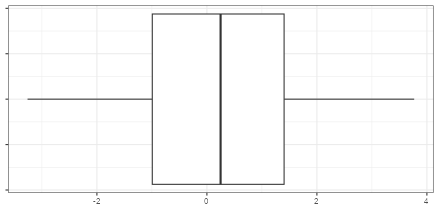
\includegraphics[width=1\linewidth]{figuras/quartis_corrupcao_judiciaria.png}
    \label{fig:quartis_corrupcao_judiciaria}
    \footnotesize{Fonte: elaboração própria baseada em \cite{judicial-corruption-score}.}
\end{figure}

A figura \ref{fig:quartis_corrupcao_judiciaria}, que mostra a distribuição do índice de corrupção judiciária, ilustra que no ano de 2024 teve um valor mínimo de -3,2610 e um máximo de 3,7690. A média dos dados foi de 0,2490. Além disso, 25\% dos valores ficaram abaixo de -0,9930 (1º quartil), enquanto 75\% dos valores foram inferiores a 1,4035 (3º quartil).

A figura \ref{fig:rule-of-law-index} mostra como a situação em 2024 do Estado de Direito no mundo.

\begin{figure}[H]
	\centering
	\caption{Estado de Direito no mundo em 2024}
	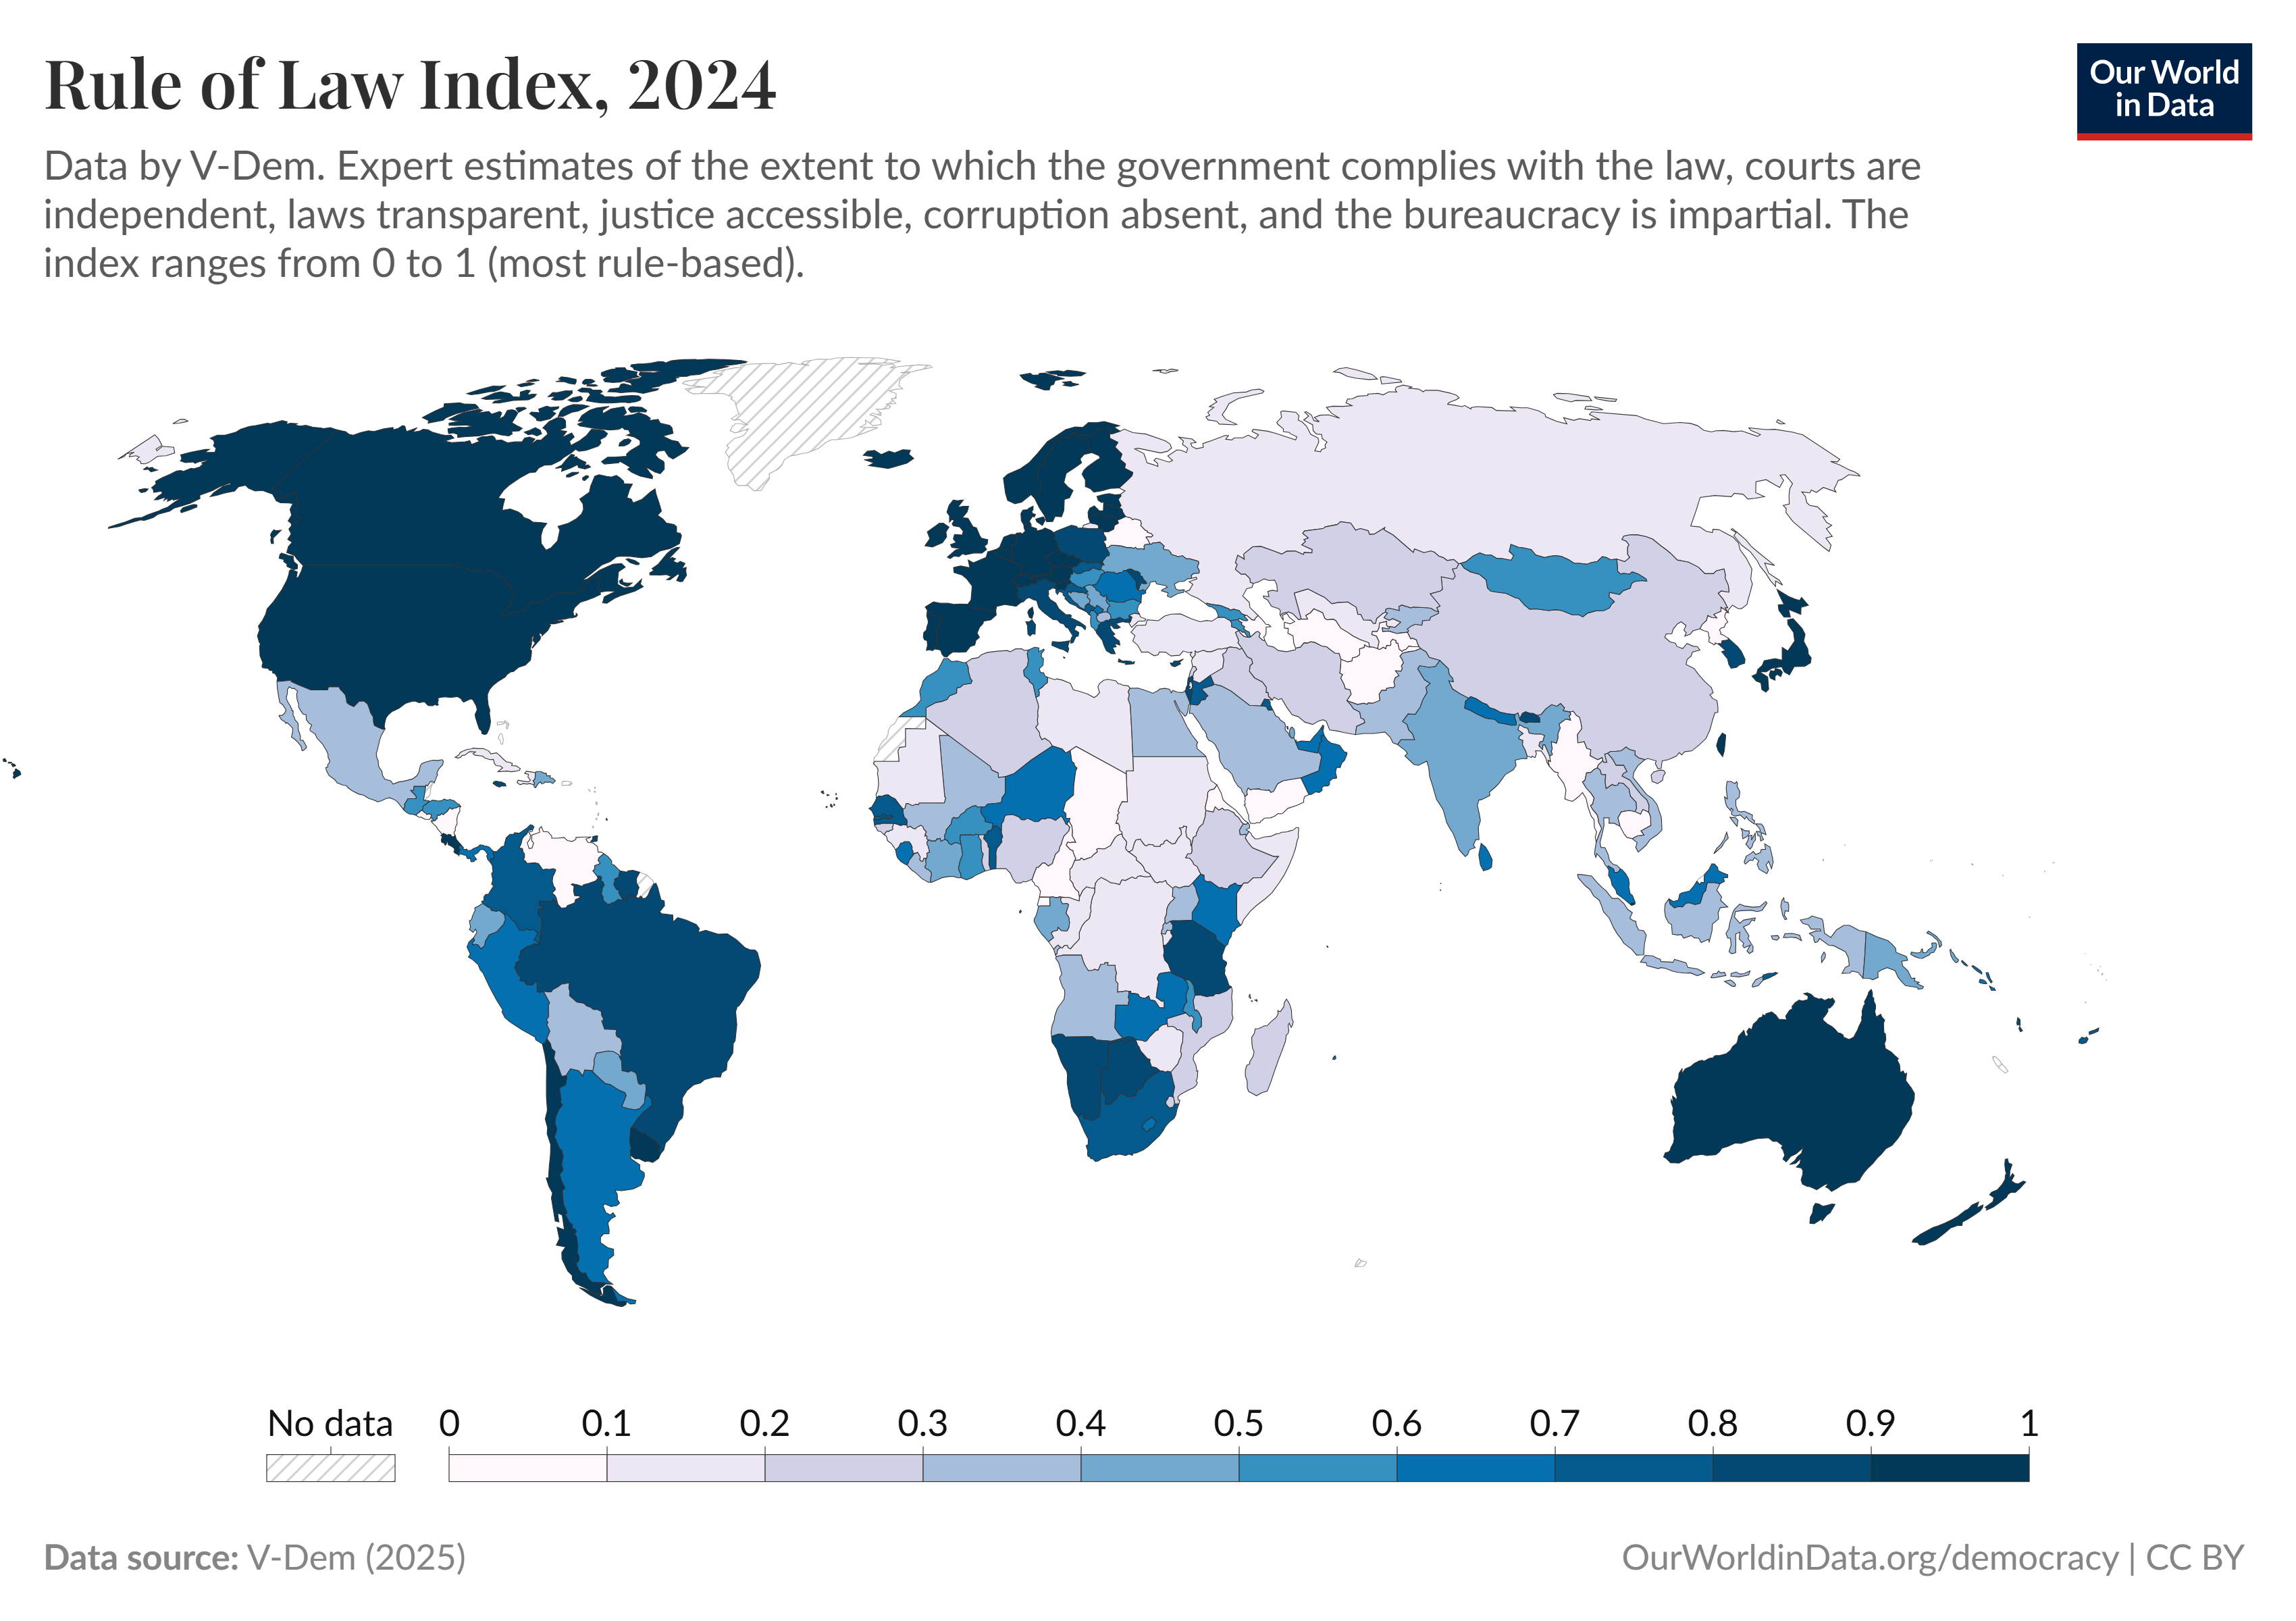
\includegraphics[width=1\linewidth]{figuras/rule-of-law-index.png}
	\label{fig:rule-of-law-index}
	\footnotesize{Fonte: \cite{rule-of-law-index}.}
\end{figure}

Nota-se como a instituição do Estado de Direito é muito fraco ou inexistente em muitos países do globo. De forma complementar a figura anterior, a figura \ref{fig:rule-of-law-index-brazil} mostra à situação histórica do Estado de Direito no Brasil (desde 1822 até 2024)

\begin{figure}[H]
	\centering
	\caption{Estado de Direito no Brasil (1822-2024)}
	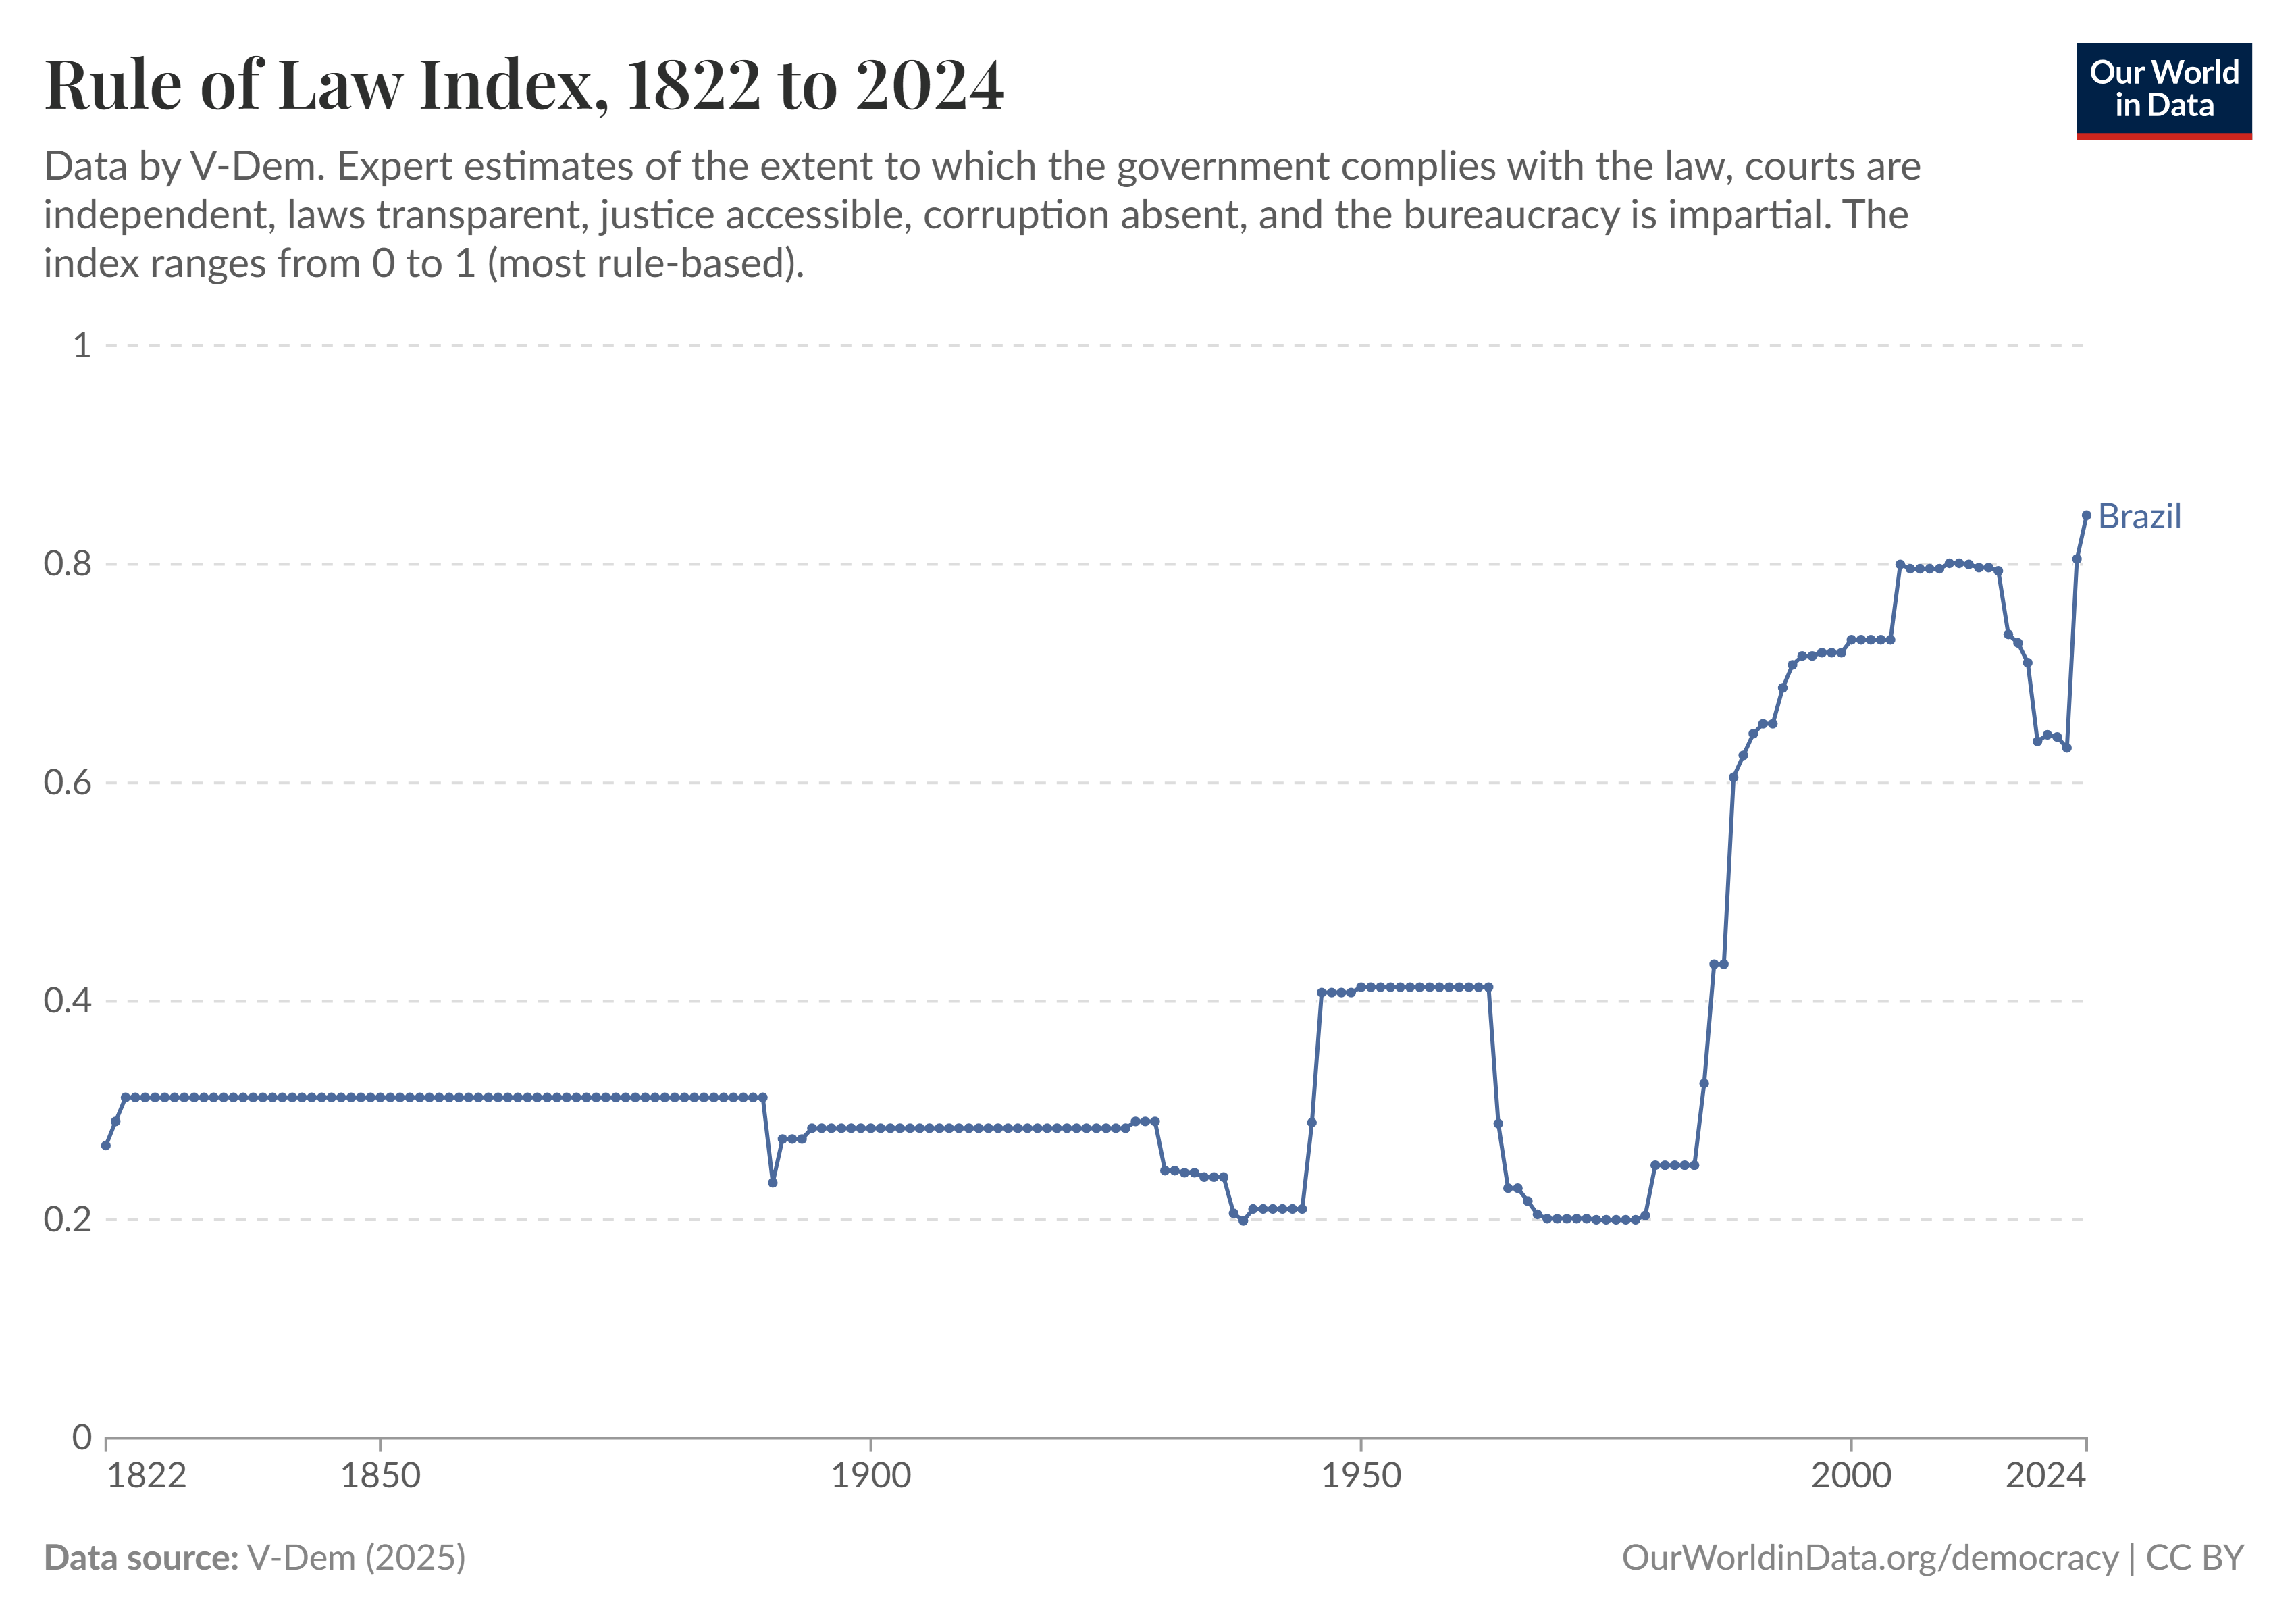
\includegraphics[width=1\linewidth]{figuras/rule-of-law-index-brazil.png}
	\label{fig:rule-of-law-index-brazil}
	\footnotesize{Fonte: \cite{rule-of-law-index}.}
\end{figure}

Nota-se como o Brasil evoluiu no aspecto do Estado de Direito. Durante mais de 100 anos (1822 até quase 1950), o Brasil ficou na baixa faixa 0,2-0,4, no entanto, atingiu o valor de 0,8 em 2023 e 0,84 em 2024 via políticas públicas que almejaram esse crescimento.

A figura \ref{fig:quartis_estado_direito} contém um gráfico de caixa.

\begin{figure}[H]
	\centering
	\caption{Gráfico da caixa: Estado de Direito}
	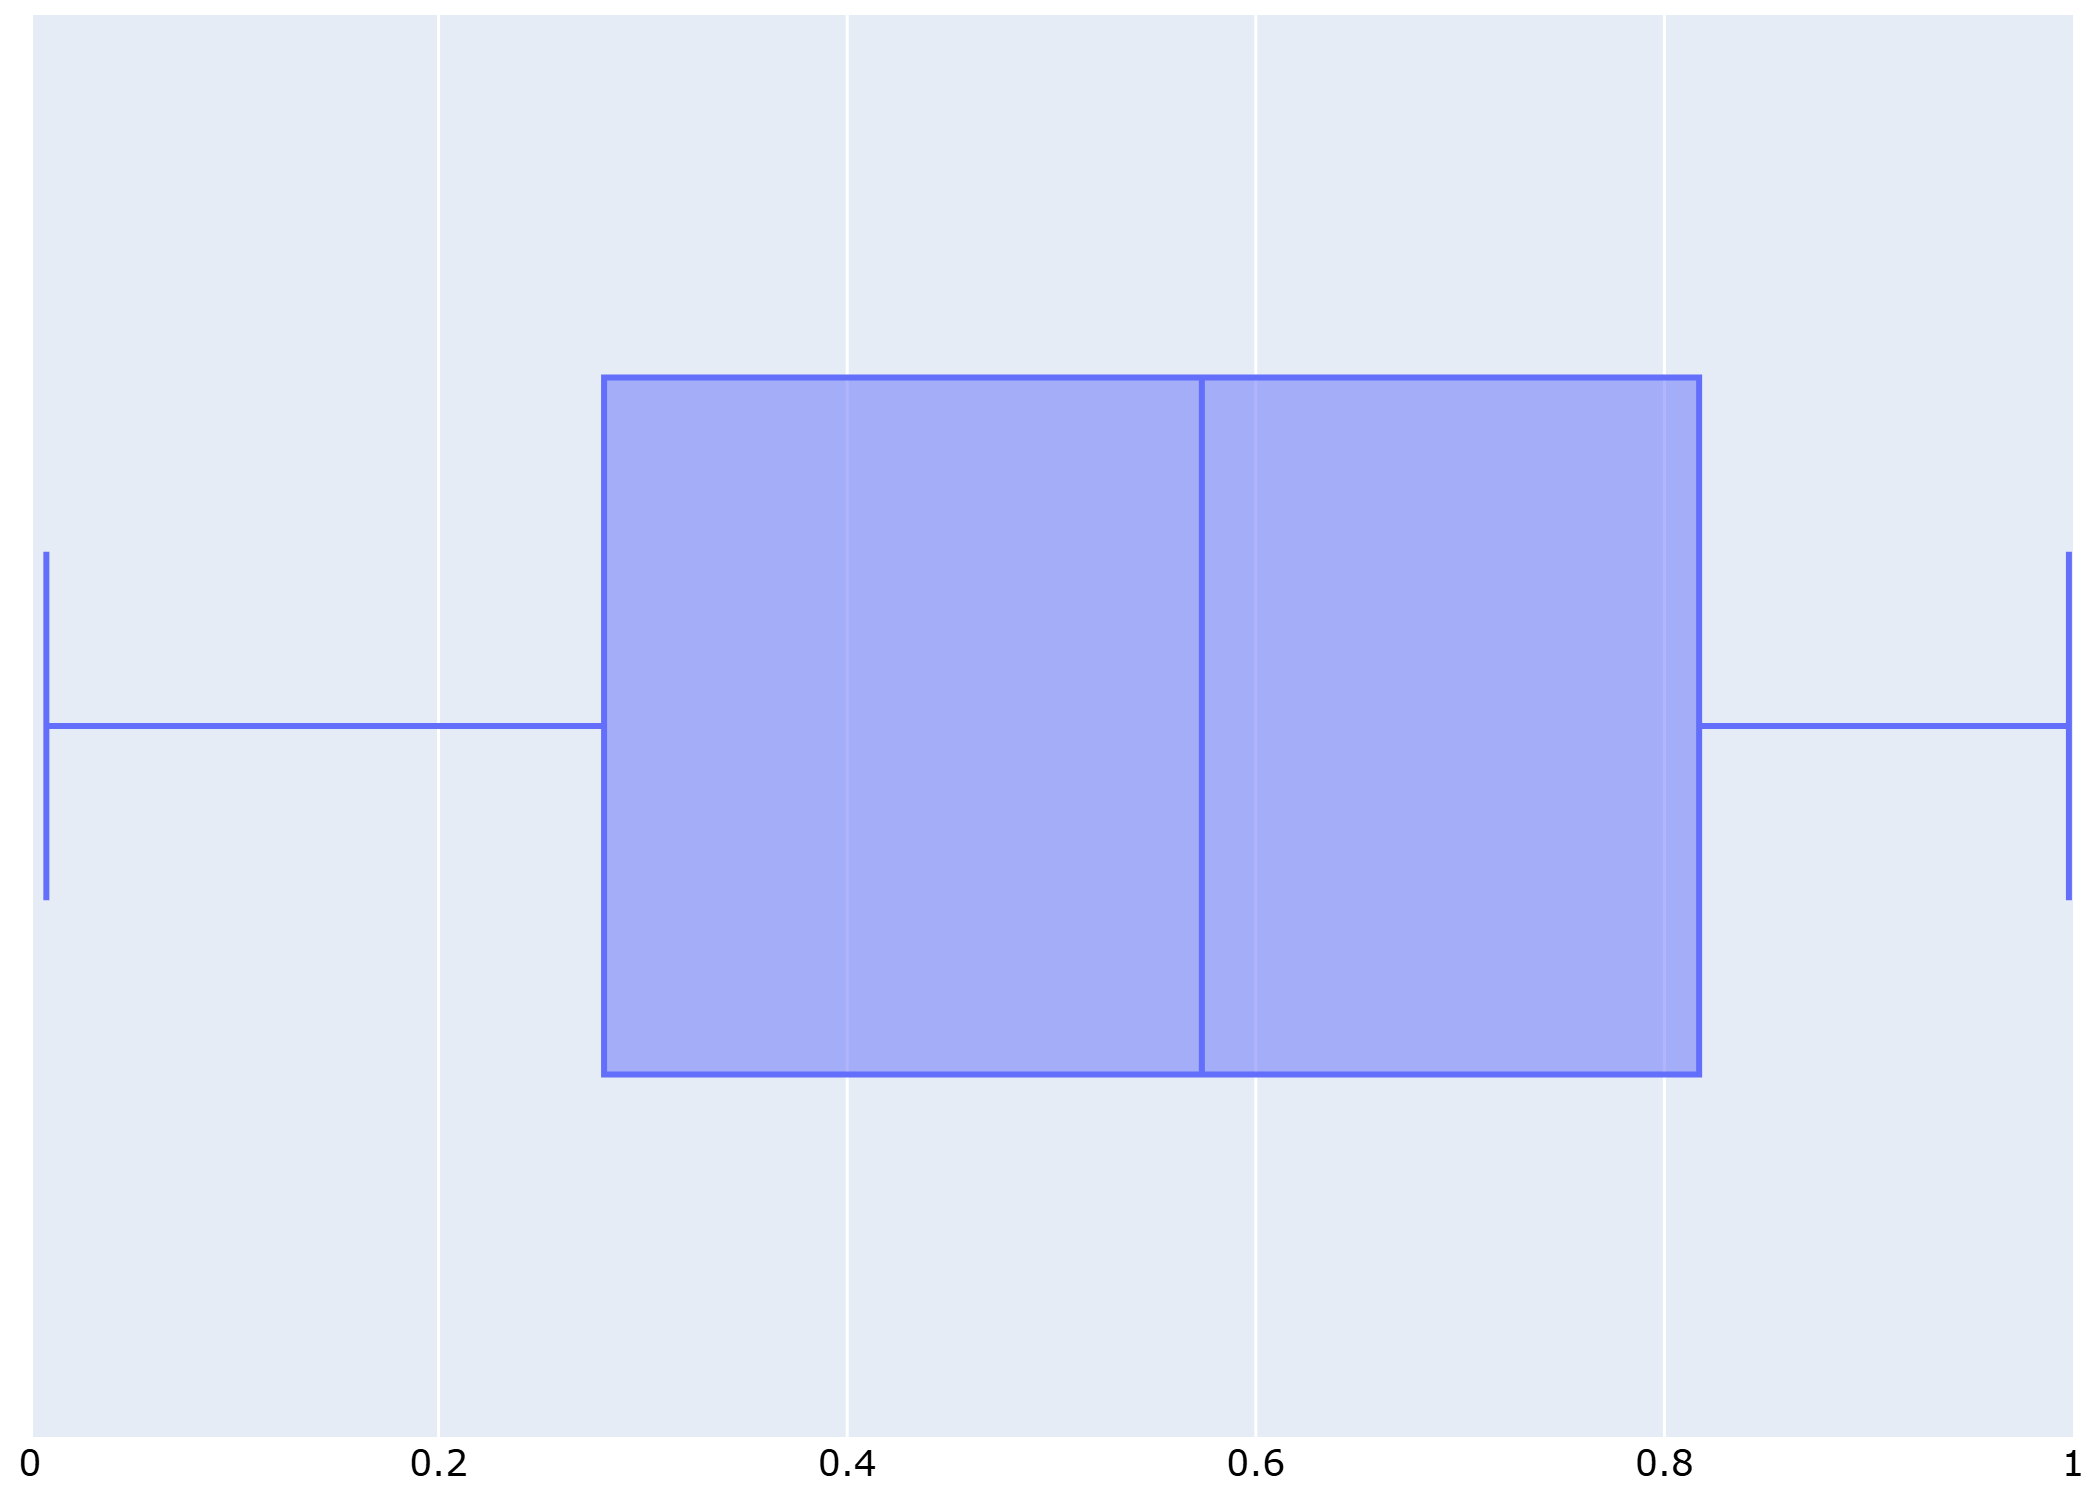
\includegraphics[width=1\linewidth]{figuras/quartis_estado_direito.png}
	\label{fig:quartis_estado_direito}
	\footnotesize{Fonte: elaboração própria baseada em \cite{rule-of-law-index}.}
\end{figure}

A figura \ref{fig:quartis_estado_direito}, que mostra a distribuição do índice de corrupção judiciária, ilustra que no ano de 2024 teve um valor mínimo de 0,008 e um máximo de 0,998. A média dos dados foi de 0,5736. Além disso, 25\% dos valores ficaram abaixo de 0,282 (1º quartil), enquanto 75\% dos valores foram inferiores a 0,816 (3º quartil).

Além da análise gráfica, estudou-se se há correlação entre o índice de democracia eleitoral com os índices de controle judicial sob o Poder Executivo, corrupção no Poder Judiciário, Estado de Direito e liberdades civis.

A figura \ref{fig:comparacao_democracia} contém um gráfico de barras que contêm os coeficientes de correlação das relações entre o índice de democracia eleitoral com os índices de controle judicial sob o Poder Executivo, corrupção no Poder Judiciário, Estado de Direito e liberdades civis.

\begin{figure}[H]
	\centering
	\caption{Coeficiente de correlação: índice de democracia eleitoral x índices de controle judicial sob o Poder Executivo, corrupção no Poder Judiciário, Estado de Direito e liberdades civis}
	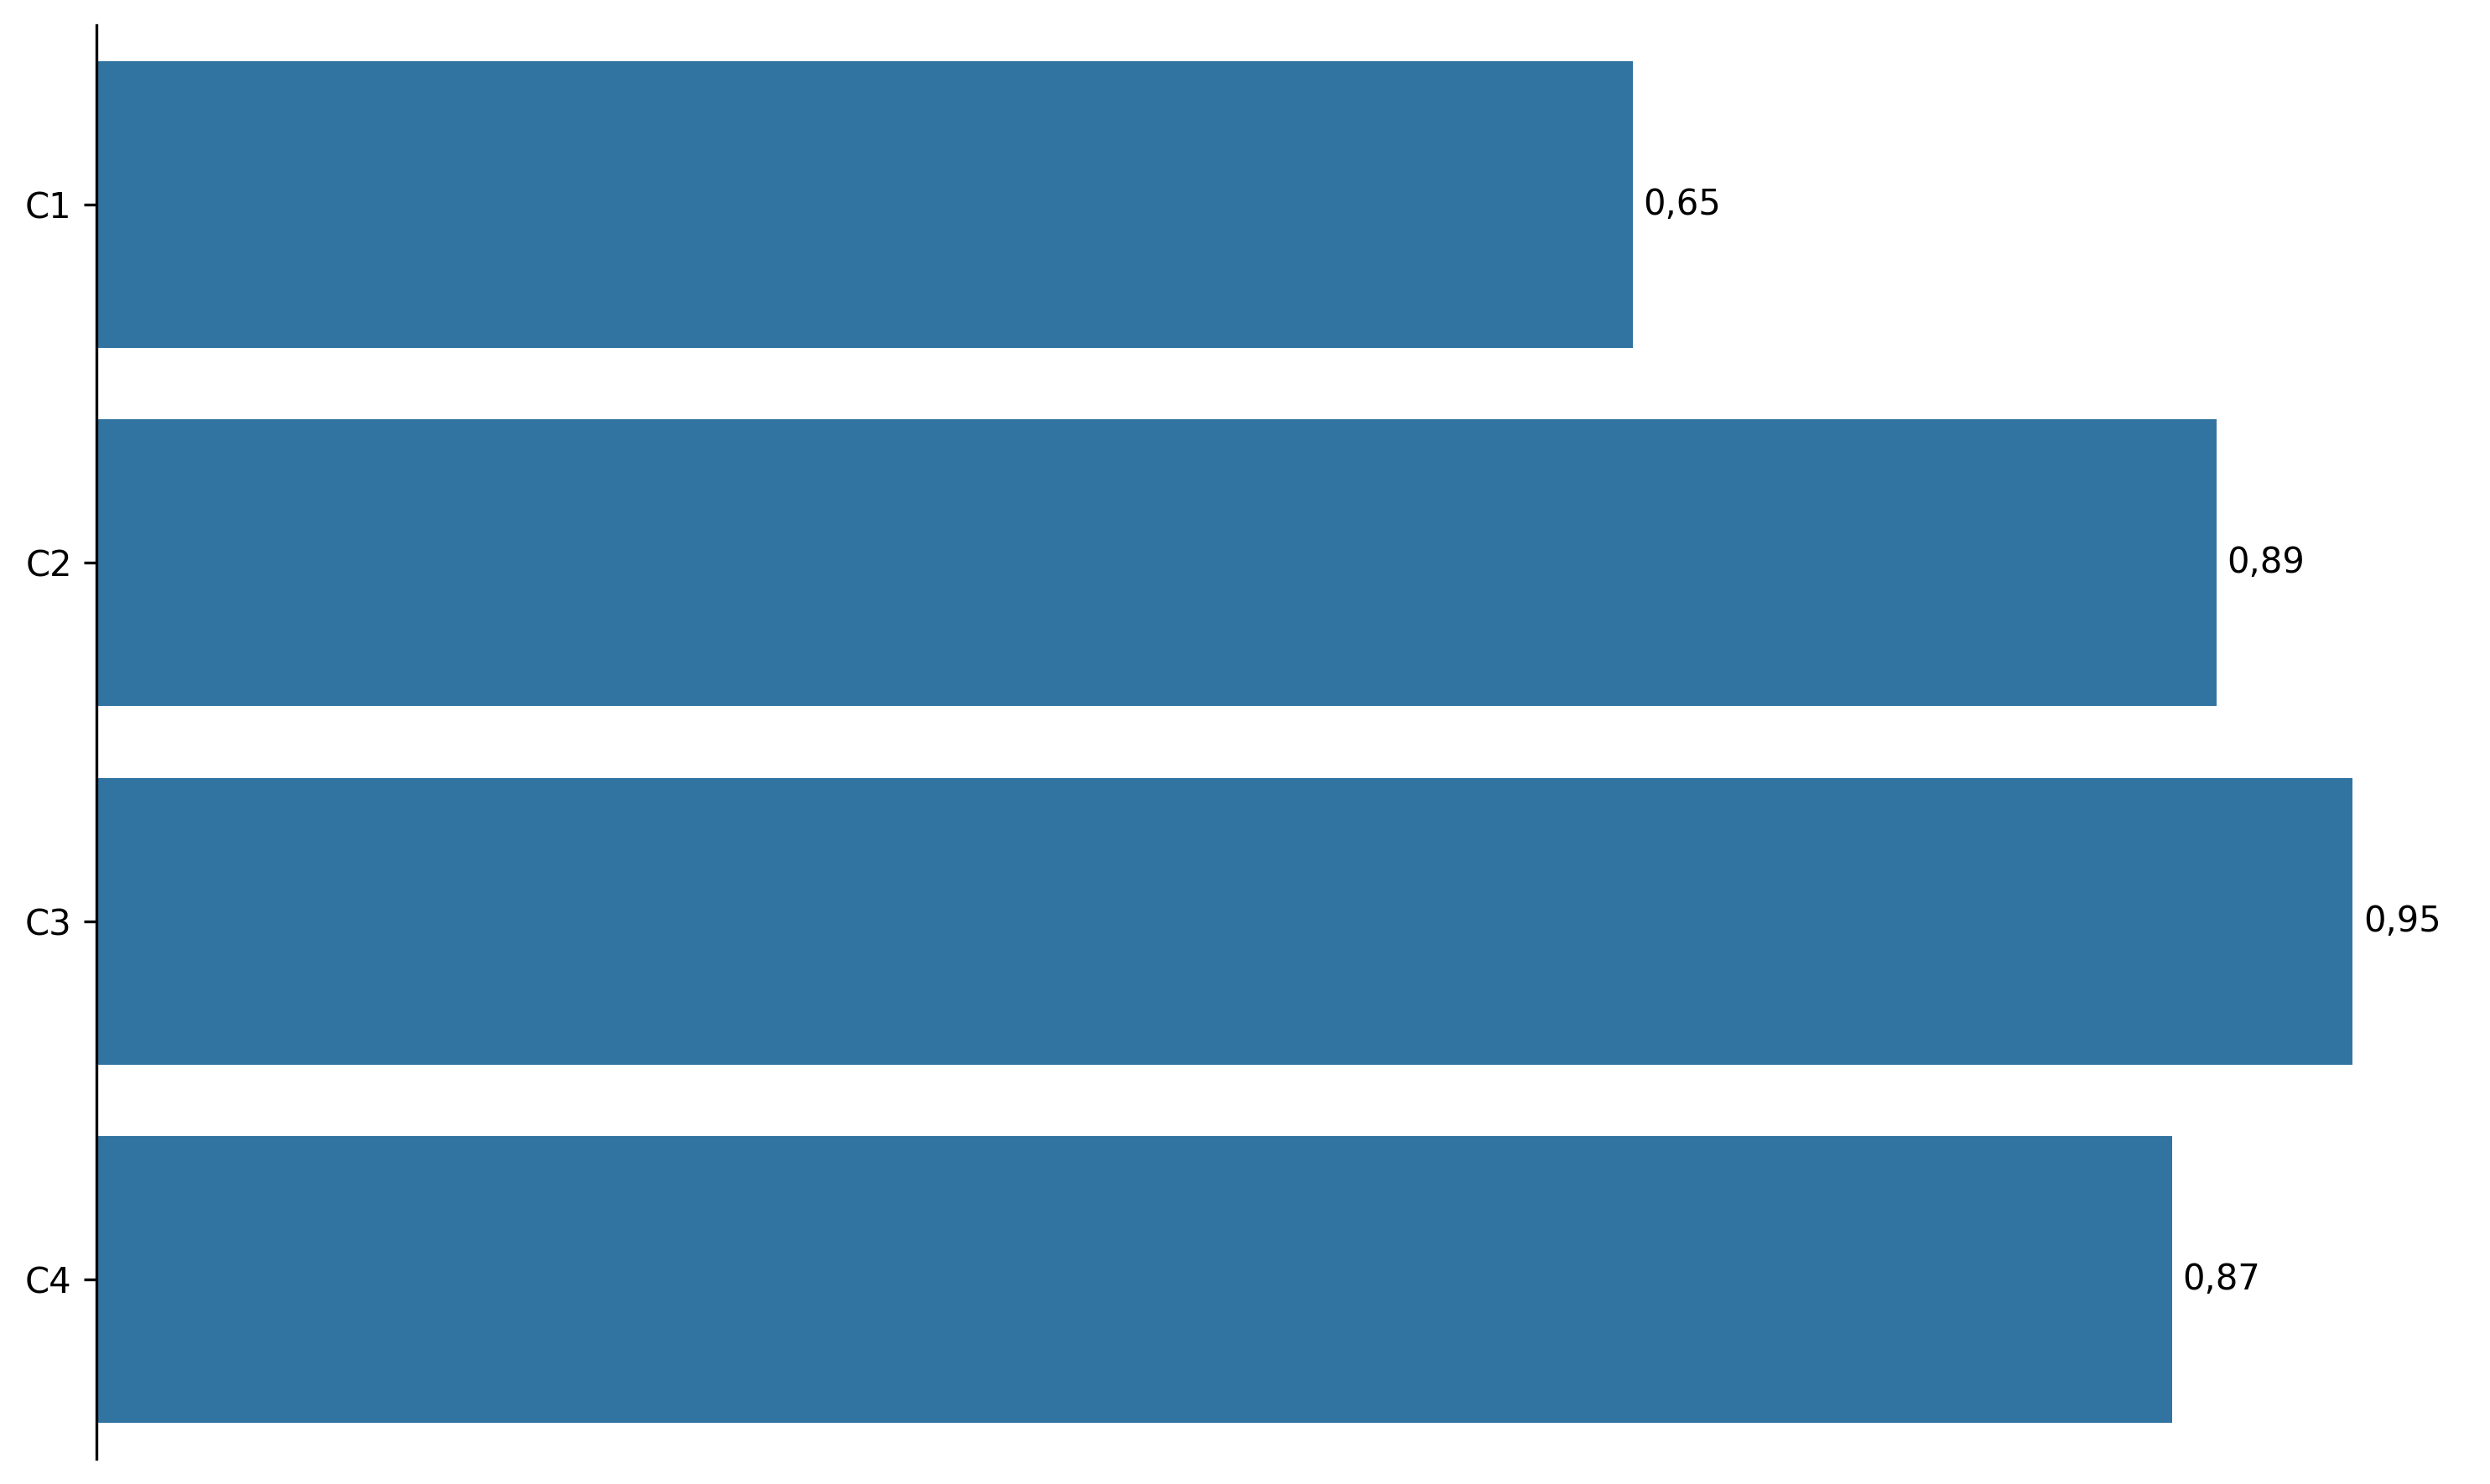
\includegraphics[width=1\linewidth]{figuras/comparacao_democracia.png}
	\label{fig:comparacao_democracia}
	\footnotesize{Fonte: elaboração própria baseada em \cite{rule-of-law-index}, \cite{jus_constraints_on_gov}, \cite{judicial-corruption-score} e \cite{human-rights-index-vdem}.}
\end{figure}

Nota-se da figura \ref{fig:comparacao_democracia} que a relação índice de democracia eleitoral x índice de corrupção judiciária tem uma correlação positiva média, enquanto as relações dos índices de controle judicial sob o Poder Executivo, liberdade civil e de Estado de Direito com o índice de democracia eleitoral tem correlações positivas fortes. Ou seja, controle judicial sob o Poder Executivo, liberdade civil e de Estado de Direito têm grande impacto na democracia. 

Considerando a análise de coeficiente de correlação anterior, destaque-se que o Brasil está em posição privilegiada, pois, se apenas 25\% dos 193 países alcançaram uma pontuação superior e metade alcançou menos que a média mundial, isso é um indicativo de que autocracias são prevalentes. \cite{nord2025democracy} informa que o Brasil, juntamente com o Equador, Lesoto e a Polônia, pararam e reverteram processos de autocratização antes da disrupção da democracia, exibindo resiliência a rupturas autocráticas.

Outros dados que reforçam a importância da democracia no Brasil foram apresentados por \cite{nord2025democracy} no relatório \textbf{Democracy Report 2025} da V-Dem relativo ao ano de 2024 na lista abaixo:

\begin{itemize}
    \item Democracias liberais representam menos de 12\% da população mundial, ou seja, menos de 900 milhões de pessoas.
    \item Democracias eleitorais representam 17\% da população mundial.
    \item 40\%  da população mundial - 3,1 bilhões de pessoas - vive em países que estão em processo de autocratização.
    \item Há mais autocracias do que democracias no mundo: 91 contra 88. Em 2023, era o contrário.
    \item O mundo tem apenas 29 liberais, o que torna o regime o mesmo comum.
    \item 72\% das pessoas no mundo vivem em autocracias, percentual mais alto desde 1978.
\end{itemize}

\section{O Poder Judiciário como garantidor de direitos do Brasil}

Dados internacionais confirma a real democracia do Brasil. \cite{rule-of-law-index} mostra na figura \ref{fig:key-features-of-liberal-democracy} como os índices de uma democracia liberal no Brasil são altos.

\begin{figure}[H]
	\centering
	\caption{Característica principal de democracia eleitoral no Brasil em 2024}
	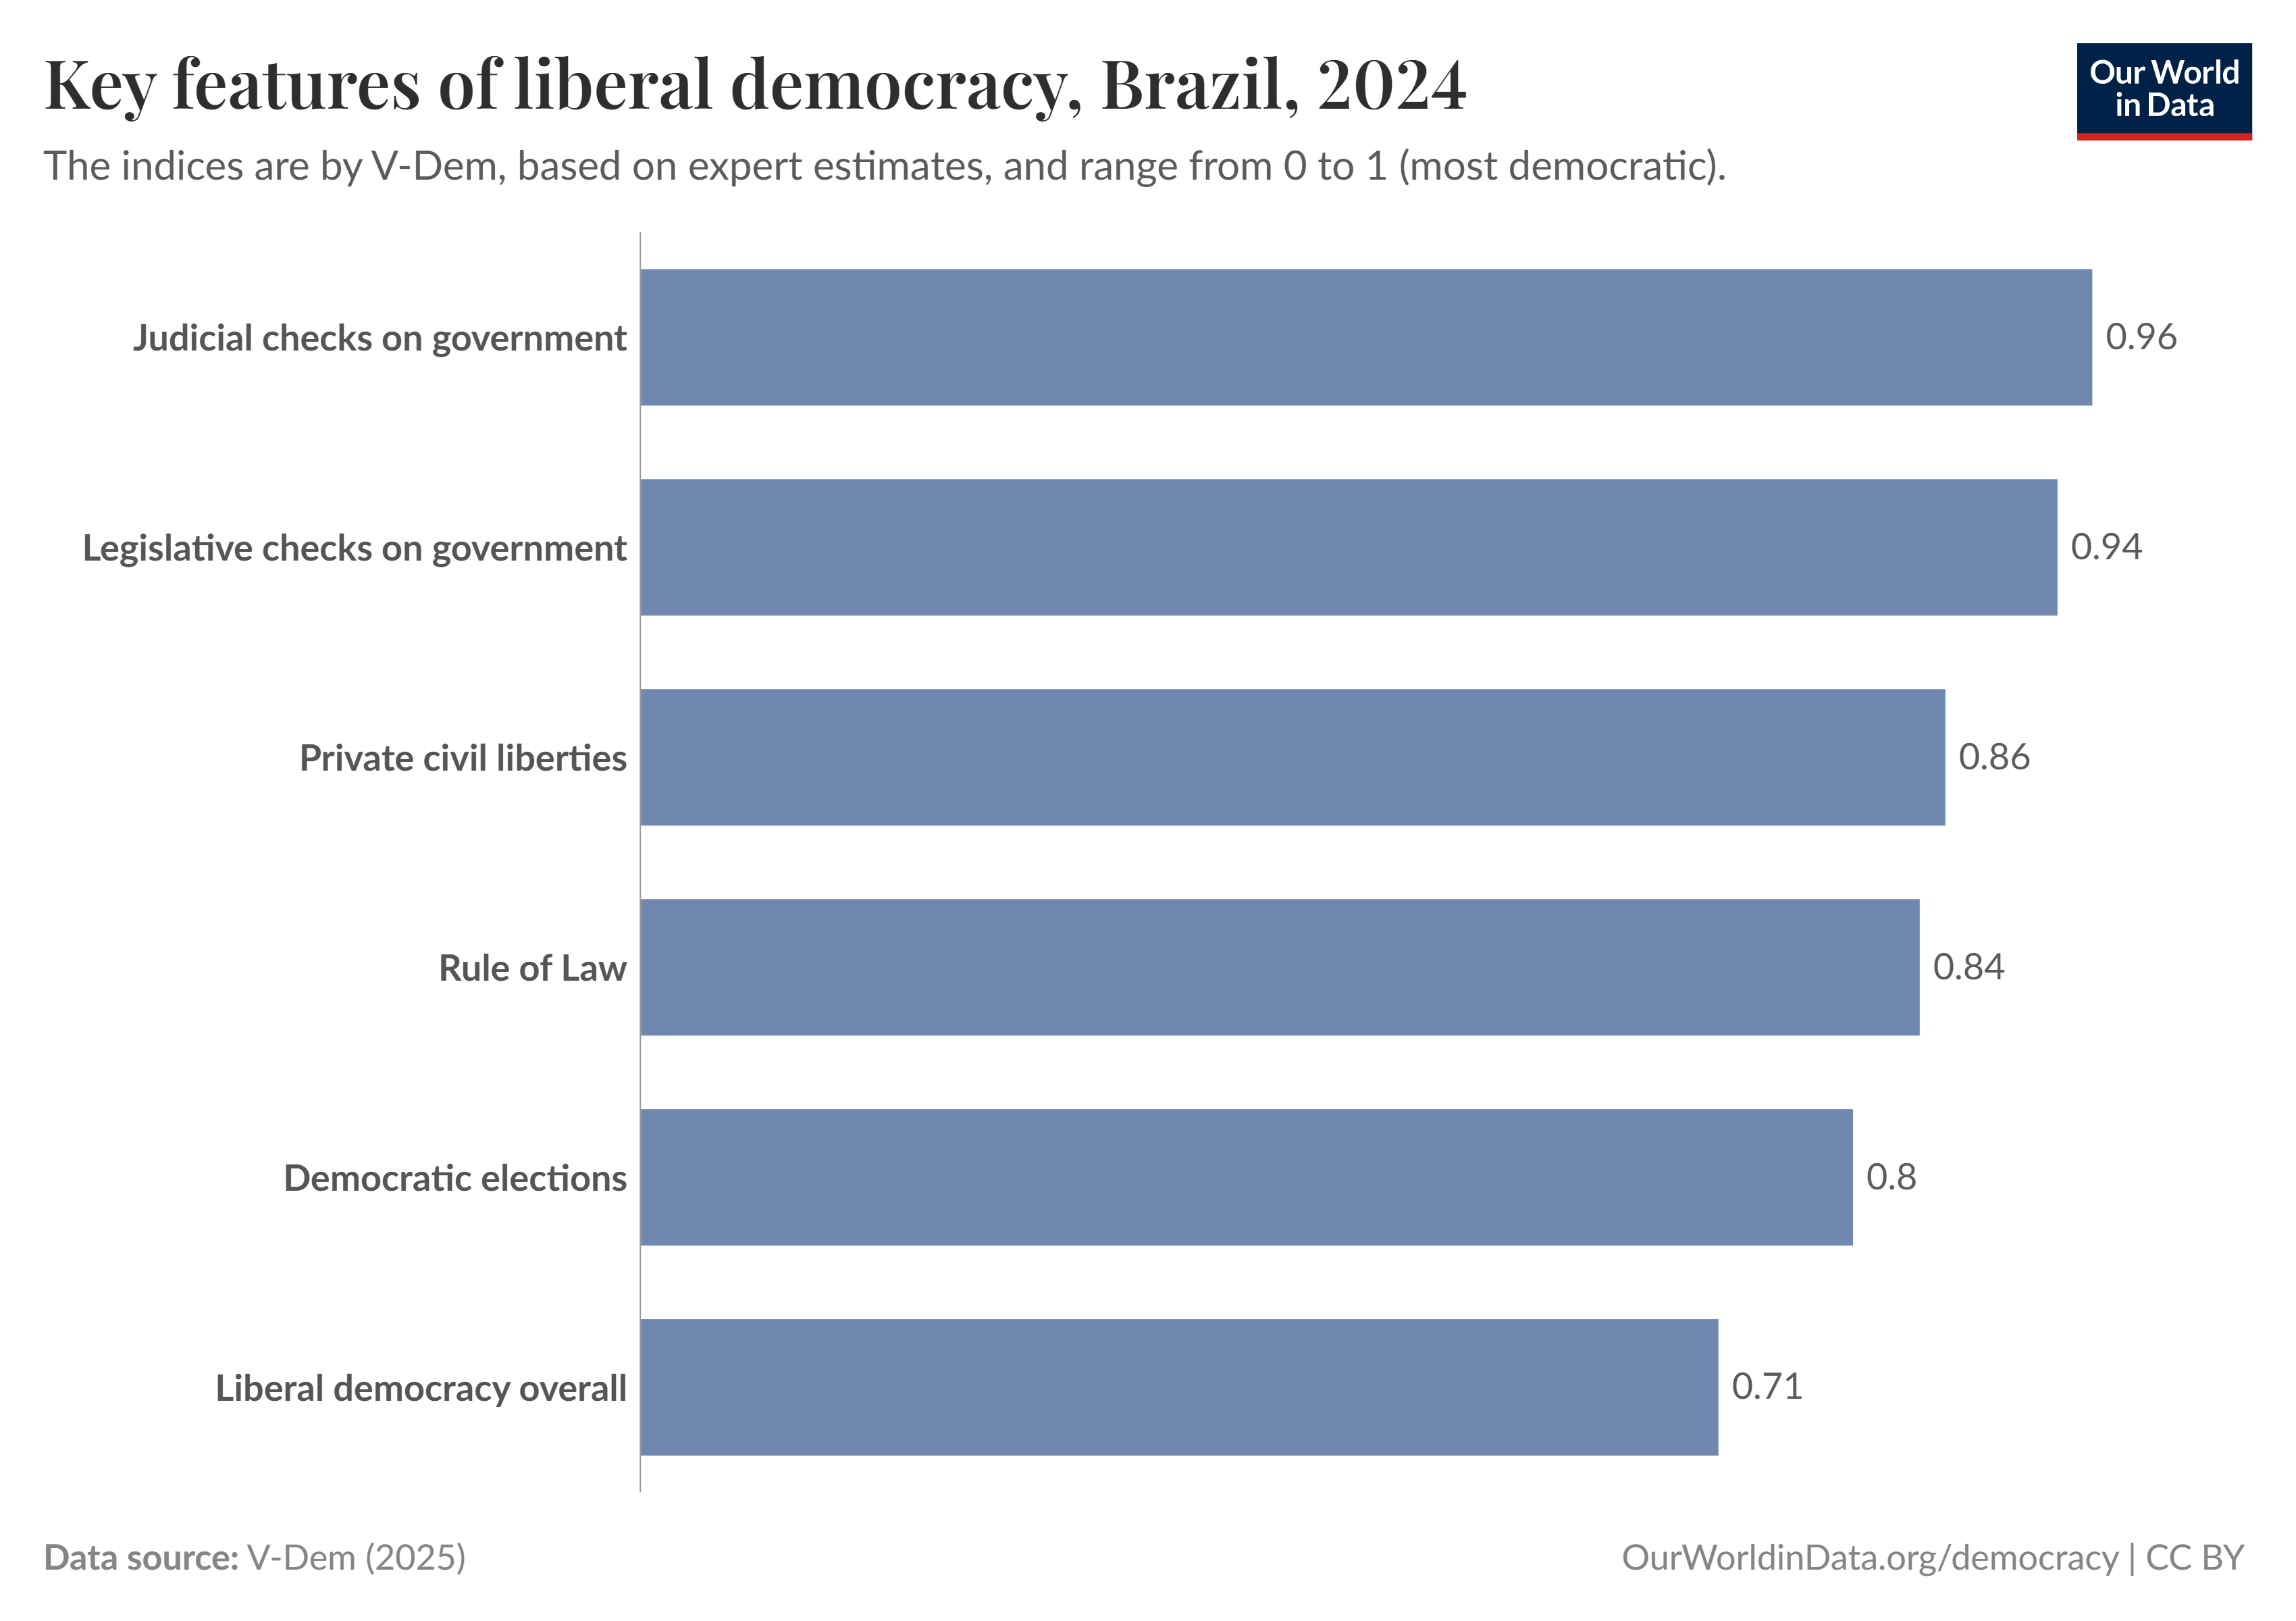
\includegraphics[width=1\linewidth]{figuras/key-features-of-liberal-democracy.png}
	\label{fig:key-features-of-liberal-democracy}
	\footnotesize{Fonte: \cite{rule-of-law-index}.}
\end{figure}

Como expresso pela figura \ref{fig:key-features-of-liberal-democracy}, além do controle judicial sobre o Poder Executivo e o Estado de Direito já citados em parágrafos anteriores, o controle legislativo sobre o Poder Executivo, as liberdades civis, as eleições democráticas são altas.

No tocante à liberdade de expressão e associação, bem como, as liberdades civis, a figura \ref{fig:comparacao_liberdade_expressao_associacao_dh}.
.
\begin{figure}[H]
	\centering
	\caption{Índice de liberdade de expressão, liberdade de associação e de liberdades civis no Brasil e a média mundial em 2024}
	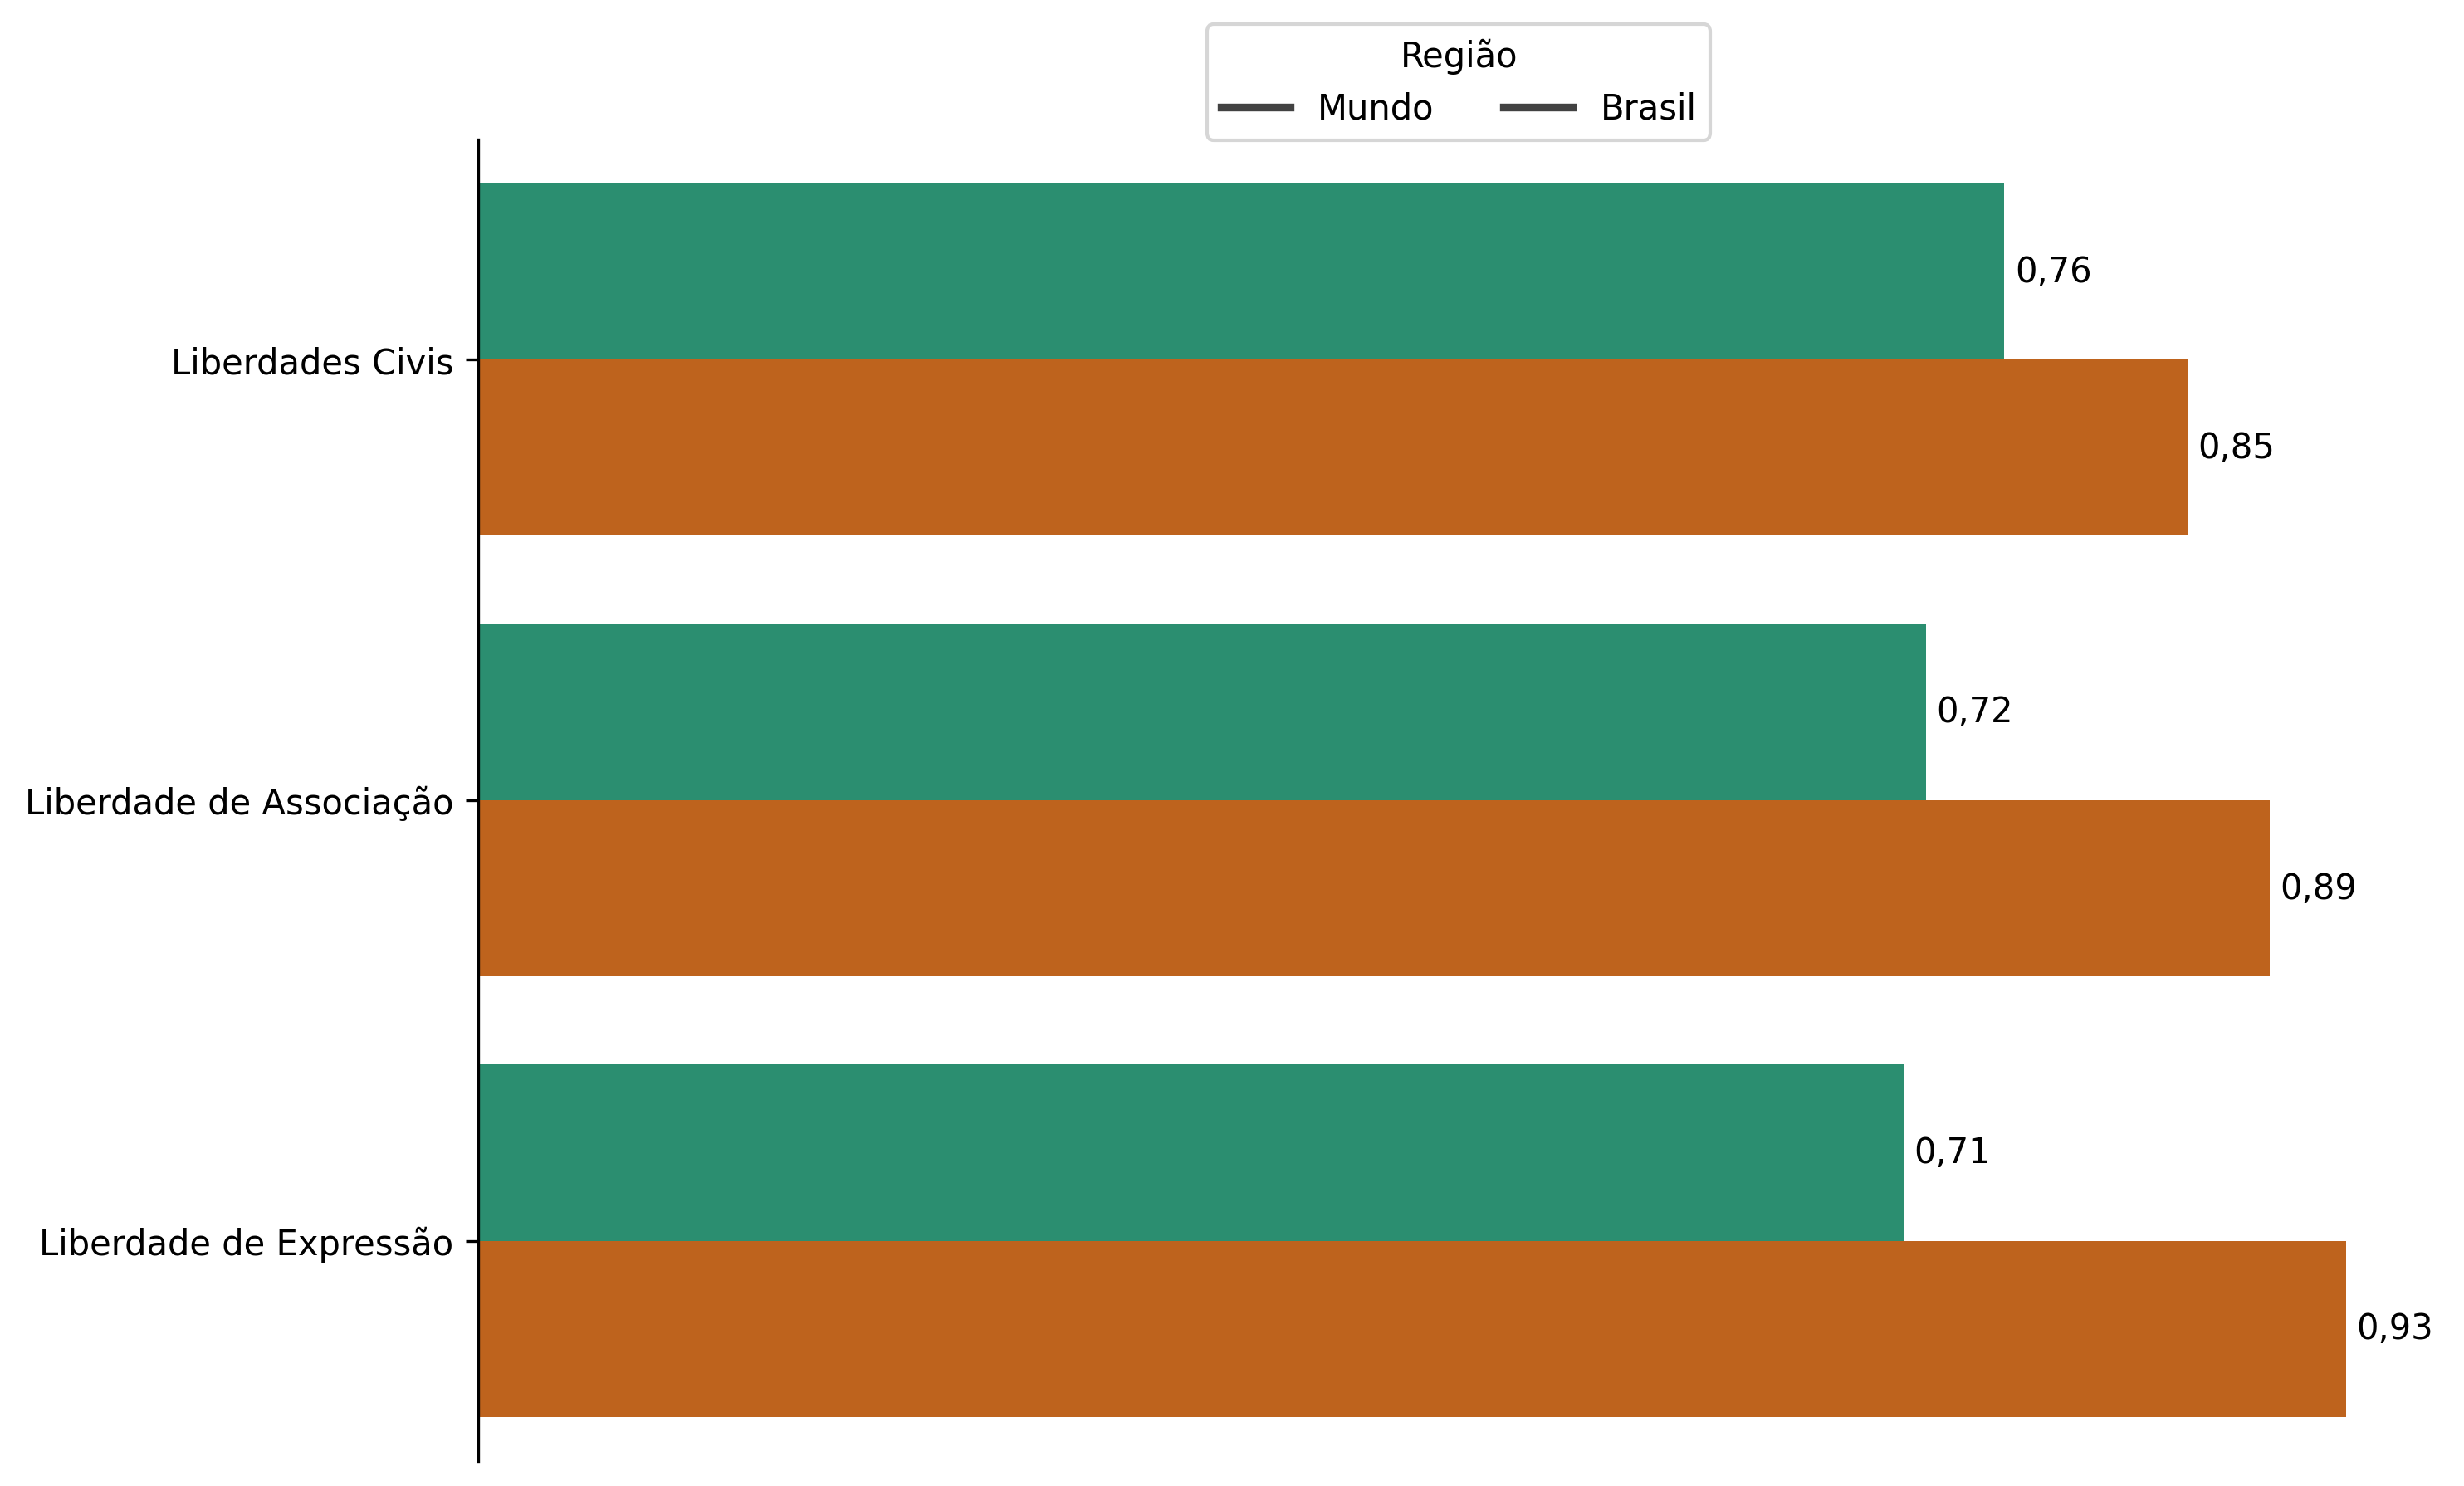
\includegraphics[width=1\linewidth]{figuras/comparacao_liberdade_expressao_associacao_dh.png}
	\label{fig:comparacao_liberdade_expressao_associacao_dh}
	\footnotesize{Fonte: elaboração própria baseada em \cite{freedom-of-association-index}, \cite{freedom-of-expression-index} e \cite{human-rights-index-vdem}.}
\end{figure}

Conforme expresso na figura \ref{fig:comparacao_liberdade_expressao_associacao_dh}, o Brasil se destaca nos quesitos liberdade de expressão e associação, bem como, os direitos humanos em relação à média mundial.

Os tópicos citados nas figuras \ref{fig:key-features-of-liberal-democracy} e \ref{fig:comparacao_liberdade_expressao_associacao_dh} representam temas ligados à Constituição Federal de 1988. Um exemplo é direito de associação, presente no art. 5º, XVII da Carta Magna, conforme \cite{cf88}, declara como plena a liberdade de associação para fins lícitos, vedada a de caráter paramilitar. O art. 37, VI, nos termos da Constituição, haja vista \cite{cf88}, garante ao servidor público civil o direito à livre associação sindical.

Outro exemplo é o do controle legislativo sobre o Poder Executivo. A Constituição Federal de 1988 concedeu ao Congresso Nacional, com auxilio do Tribunal de Contas da União, haja vista \cite{cf88}, poder fiscalizador sob o Poder Executivo via comissões permanentes, temporárias, especiais e as de inquérito parlamentar.

A Constituição Federal de 1988, assim argumentado por \cite{cf88}, concedeu competência constitucional para o Congresso Nacional sustar os atos normativos do Poder Executivo que exorbitem do poder regulamentar ou dos limites de delegação legislativa.

Ao Congresso Nacional, segundo \cite{cf88}, cabe sustar os efeitos jurídicos, respeitados os direitos adquiridos, de medidas provisórias expedidas pelo Presidente da Republica. E, por fim, conduzir a remoção do cargo de Presidente da República do seu ocupante.

As informações alarmantes apresentadas por \cite{nord2025democracy} expõem o quão benéfica tem sido a democracia para o Brasil desde a redemocratização. Embora o Brasil ainda apresente desafios, o país está em processo de melhoria institucional. Um exemplo disso é o fato do Brasil ter tido a capacidade de reverter uma tentativa de autocratização enquanto 40\%  da população mundial vive em países que estão em processo de autocratização.

Como consequência da argumentação anterior, \cite{pires2021paradoxo} corrobora a independência do Poder Judiciário. Para o autor, o Poder Judiciário obteve níveis elevados de independência com a Constituição Federal de 1988, que em um esforço para fortalecer a independência individual dos juízes, os termos e condições de mandato foram significativamente aprimorados.  Bem como, a Constituição Federal também fortaleceu a independência funcional do judiciário como instituição de governança, isolando-o do sistema político mais amplo.

No tocante aos direitos humanos, algumas decisões de caráter nacional foram aprovadas. Na ADPF 527, de acordo com \cite{adpf527}, "Assim, com base em diálogo institucional estabelecido com o Poder Executivo, como explicitado acima, ajusto os termos da cautelar já deferida para outorgar às transexuais e travestis com identidade de gênero feminina o direito de opção por cumprir pena: (i) em estabecimento prisional feminino; ou (ii) em estabelecimento prisional masculino, porém em área reservada, que garanta a sua segurança."

Outra decisão afeta aos direitos é a jurisprudência do STJ em relação a interpretação judicial e a aplicação do art. 318-A do Código de Processo Penal, introduzido pela Lei nº 13.769, de 2018, haja vista \cite{cpp}:

\noindent
\begin{flushleft}
\setlength{\leftskip}{4cm}
\small
"Art. 318-A.  A prisão preventiva imposta à mulher gestante ou que for mãe ou responsável por crianças ou pessoas com deficiência será substituída por prisão domiciliar, desde que: (Incluído pela Lei nº 13.769, de 2018).

I - não tenha cometido crime com violência ou grave ameaça a pessoa;              (Incluído pela Lei nº 13.769, de 2018).

II - não tenha cometido o crime contra seu filho ou dependente. (Incluído pela Lei nº 13.769, de 2018)." \cite{cpp}
\end{flushleft}

Visando a plena garantia dos direitos humanos por mulheres que são mães ou responsáveis legais, o STJ tem diversas decisões que usaram o art. 318-A do Código de Processo Penal. 

O RHC 145.931/MG, de 2021, aplicou o art. 318-A do Código de Processo Penal, cujo texto da ementa segue abaixo:

\noindent
\begin{flushleft}
\setlength{\leftskip}{4cm}
\small
"RECURSO EM HABEAS CORPUS. EXECUÇÃO PENAL.	EXECUÇÃO DE PENA PRIVATIVA DE LIBERDADE DE 9 ANOS DE RECLUSÃO. REGIME INICIAL FECHADO. CONDENAÇÃO PELA PRÁTICA DOS CRIMES DE TRÁFICO DE DROGAS E ASSOCIAÇÃO PARA O TRÁFICO. PRETENSÃO DE CONCESSÃO DE PRISÃO DOMICILIAR. PACIENTE GENITORA DE CRIANÇAS DE 6 E 2 ANOS DE IDADE. POSSIBILIDADE. CARACTERIZADA INEFICIÊNCIA ESTATAL EM DISPONIBILIZAR VAGA À RECORRENTE EM ESTABELECIMENTO PRISIONAL PRÓPRIO E ADEQUADO À SUA CONDIÇÃO PESSOAL, DOTADOS DE ASSISTÊNCIA MÉDICA PRÉ-NATAL E PÓS-PARTO, BERÇÁRIOS E CRECHES. ARTS. 82, § 1º, E 83, § 2º, DA LEP. PRESÍDIO FEMININO MAIS PRÓXIMOS DISTANTE 230 KM DA RESIDÊNCIA. CONVIVÊNCIA E AMAMENTAÇÃO IMPOSSIBILITADA. PROTEÇÃO INTEGRAL À CRIANÇA. PRIORIDADE. HC COLETIVO STF N. 143.641/SP. PRECEDENTES DO STJ. LIMINAR DEFERIDA. PARECER MINISTERIAL PELA CONCESSÃO DA ORDEM, EM MENOR EXTENSÃO, A FIM DE QUE A CORTE DE JUSTIÇA SEJA INSTADA A EXAMINAR O MÉRITO DO WRIT IMPETRADO NAQUELA INSTÂNCIA NO TOCANTE À TESE ALEGADA NA INICIAL DA AÇÃO MANDAMENTAL. ILEGALIDADE MANIFESTA 	EVIDENCIADA. RECURSO PROVIDO." \cite{rhc145931}
\end{flushleft}

Evidencia-se da análise da ementa que a mulher julgada foi está sendo condenada por tráfico de drogas e associação ao tráfico, porém na condição de genitora de duas crianças de 2 e 6 anos, foi-lhe concedida a possibilidade de responder em prisão domiciliar, conforme é demostrado abaixo:

\noindent
\begin{flushleft}
\setlength{\leftskip}{4cm}
\small
"2. Ademais, o CPP (com as alterações promovidas pela Lei nº 13.769/2018) passou a prever a substituição da prisão preventiva  por domiciliar à mulher gestante, mãe ou responsável por crianças ou pessoas com deficiência, desde que não tenha cometido crime com violência ou grave ameaça e o delito não tenha sido cometido o crime 	contra seu filho ou dependente, facultando, ainda, a aplicação de medidas cautelares (arts. 318-A e 318-B do CPP)." \cite{rhc145931}
\end{flushleft}

O posicionamento do Superior Tribunal foi reiterado por outra decisão, a Reclamação nº 40.676/SP.

\noindent
\begin{flushleft}
\setlength{\leftskip}{4cm}
\small
"1. A jurisprudência desta Corte tem se orientado no sentido de que deve ser dada uma interpretação extensiva tanto ao julgado proferido pelo Supremo Tribunal Federal no Habeas Corpus coletivo n. 143.641, que somente tratava de prisão preventiva de mulheres gestantes ou mães de crianças de até 12 anos, quanto ao art. 318-A do Código de Processo Penal, para autorizar também a concessão de prisão domiciliar às rés em execução provisória ou definitiva da pena, ainda que em regime fechado." \cite{reclamacao40676}
\end{flushleft}

Nota-se como a instância superior da Justiça Comum tem foco na dignidade da pessoas humana ao estabelecer como padrão de julgamento a aplicação plena do art. 318-A do Código de Processo Penal, focando na necessidade dos filhos e dependentes legais das mulheres rés na Justiça Criminal, concomitantemente, na condição de responsável e cuidadora de pessoas das rés de pessoas que delas dependem.

De forma complementar, o STF expediu em 2018 o HC nº 143.641/SP. De acordo com \cite{hc143641}, a determinação da Suprema Corte deu-se devido a reclamação das defensorias públicas dos Estados e da União de que as apenadas estavam sofrendo graves de violações dos direitos como gestantes e que seus filhos estariam sendo afetados por extensão, de modo que suas penas em unidades prisionais poderiam ser substituídas por penas alternativas, ou por estarem em prisão preventiva, seriam absorvidas depois. 
	
Outro fatores que motivaram a reclamação perante o Supremo Tribunal Federal, segundo \cite{hc143641}, foram as condições precárias das unidades prisionais que afetam tanto as apenadas, quanto sua prole. Adicionalmente, as apenas estavam tendo outros direitos que estão sendo desrespeitados, não se podendo penalizá-las pela falta de estrutura estatal adequada para fazê-los valer.

Complementarmente, haja vista \cite{hc143641}, foi argumentado que é o direito de punir, e não o direito à vida, à  integridade e à liberdade individual, que deve ser mitigado. Além disso, os reclamantes destacaram também a vulnerabilidade socioeconômica das mulheres presas preventivamente no Brasil. Requereram, por fim, a concessão da ordem para revogação da prisão preventiva decretada contra todas as gestantes puérperas e mães de crianças, ou sua substituição pela prisão domiciliar

Como resultado da independência proporcionada pela Constituição Federal, \cite{pires2021paradoxo} cita que os tribunais receberam controle total sobre seus assuntos administrativos, pessoais e disciplinares, de modo que o Poder Judiciário obteve controle quase total sobre seu orçamento.

No tocante à liberdade de expressão, \cite{daliberdade} cita que, na condição de um dos mais prestigiados direitos das sociedades democráticas, a liberdade de expressão encontra tutela na Constituição Federal, cujo art. 5º, inciso IV, dispõe que “é livre a manifestação do pensamento, sendo vedado o anonimato”.

Para \cite{daliberdade}, o direito à liberdade de expressão, que possui destacada função na concretização do Estado Democrático, em muitas situações se revela em rota de colisão com outros direitos de mesma hierarquia constitucional, principalmente quando está em jogo a delimitação da sua amplitude. 

Nesse sentido, em concordância com \cite{daliberdade}, Para a Corte Suprema, como visto, as linhas que autorizam restrições ao exercício da liberdade de expressão são bastante estreitas. Nesse contexto, o Tribunal não tem admitido proteção à liberdade de expressão em atos de incitação ao ódio, à intolerância e a violência, assim como tem vedado - para além do campo jurídico - manifestações que denotem conteúdo imoral, devendo, ainda, tal liberdade ser pautada pelo resguardo de outros direitos
fundamentais, como a honra, à intimidade e a privacidade.

Um exemplo da ação do Supremo Tribunal Federal foi a equiparação do crime de homofobia com o racismo, com base na Lei nº 7.716, de 1989. Conforme \cite{ado26}:

\noindent
\begin{flushleft}
\setlength{\leftskip}{4cm}
\small
"1. Até que sobrevenha lei emanada do Congresso Nacional destinada a
implementar os mandados de criminalização definidos nos incisos XLI e XLII do
art. 5º da Constituição da República, as condutas homofóbicas e transfóbicas, reais ou
supostas, que envolvem aversão odiosa à orientação sexual ou à identidade de gênero de
alguém, por traduzirem expressões de racismo, compreendido este em sua dimensão
social, ajustam-se, por identidade de razão e mediante adequação típica, aos preceitos
primários de incriminação definidos na Lei nº 7.716, de 08/01/1989, constituindo,
também, na hipótese de homicídio doloso, circunstância que o qualifica, por configurar motivo torpe (Código Penal, art. 121, § 2º, I, “in fine”);" \cite{ado26}
\end{flushleft}

Outra marco ligado à liberdade de impressa foi a declaração de não-recepção pela Constituição Federal de 1988 da Lei nº 5.250, de 1967 - conhecida como Lei da Impressa. O Supremo Tribunal Federal aprovou a ADPF 130/DF visando garantir a liberdade de impressa no Brasil. Segundo \cite{adpf130}:

\noindent
\begin{flushleft}
\setlength{\leftskip}{4cm}
\small
"Tirante, unicamente, as restrições que a Lei Fundamental de 1988 prevê para o 'estado de sítio' (art. 139), o Poder Público somente pode dispor sobre matérias lateral ou reflexamente de imprensa, respeitada sempre a ideia-força de que quem quer que seja tem o direito de dizer o que quer que seja. Logo, não cabe ao Estado, por qualquer dos seus órgãos, definir previamente o que pode ou o que não pode ser dito por indivíduos e jornalistas. As matérias reflexamente de imprensa, suscetíveis, portanto, de conformação legislativa, são as indicadas pela própria Constituição, tais como: direitos de resposta e de indenização, proporcionais ao agravo; proteção do sigilo da fonte ("quando necessário ao exercício profissional"); responsabilidade penal por calúnia, injúria e difamação; diversões e espetáculos
públicos; estabelecimento dos "meios legais que garantam à pessoa e à família a possibilidade de se defenderem de programas ou programações de rádio e televisão que contrariem o disposto no art. 221, bem como da propaganda de produtos, práticas e serviços que possam ser nocivos à saúde e ao meio ambiente" (inciso II do § 3º
do art. 220 da CF); independência e proteção remuneratória dos profissionais de imprensa como elementos de sua própria qualificação técnica (inciso XIII do art. 5º); participação do capital estrangeiro nas empresas de comunicação social (§ 4º do
art. 222 da CF); composição e funcionamento do Conselho de Comunicação Social (art. 224 da Constituição)." \cite{ado26}
\end{flushleft}

\cite{da2023cadernos} cita outras julgados do STF relativos à liberdade de expressão no periódico \textbf{Cadernos de Jurisprudência do Supremo Tribunal Federal: Concretizando Direitos Humanos} cuja temática é a \textbf{liberdade de expressão, democracia e novas tecnologias}, tais como o HC nº 82.424, o RE nº 511.961, as ADPF nº 187, 4.815, as ADI nº 5.122, 2.566, 4.451, por exemplo.

Como forma de evitar a ingerência do Poder Executivo, \cite{pires2021paradoxo} argumenta que a Constituição Federal estabeleceu o STF é o responsável pela elaboração do orçamento anual da Justiça Federal e pelo encaminhamento direto ao Congresso Nacional. Assim, limitou-se o poder do Governo Federal sob o Poder Judiciário. 

Outro autor destacou a importância da independência do Poder Judiciário foi \cite{akutsu2012dimensoes}. Para ele, a importância de um Poder Judiciário independente dos Poderes Executivo e Legislativo decorre da necessidade de salvaguarda da liberdade individual dos cidadãos, que podem recorrer ao Judiciário contra abusos de autoridades de quaisquer dos três poderes. 

Para \cite{akutsu2012dimensoes}, a independência do Poder Judiciário não deve constituir óbice do cumprimento dos princípios e às normas da Constituição Federal pelos juízes. Além de poder serem responsabilizados perante os cidadãos. 

Complementarmente, para \cite{akutsu2012dimensoes} no caso da premissa da independência dos juízes e tribunais não se concretize, o desempenho do Poder Judiciário pode ser afetado, uma vez que os juízes enfrentariam óbices para  proferir sentenças que desagradassem pessoas afetadas por suas decisões.

Como fortalecedor da independência do Poder Judiciário, e como demonstração constitucional de sua importância para o Brasil, em 2004 o Congresso Nacional aprovou a Emenda à Constituição nº 45, de 2004. \cite{ec45_2004} criou o CNJ, as Súmulas Vinculantes do STF, extinguiu os Tribunais de Alçada e determinou sua incorporação aos Tribunais de Justiça, além das outras medidas estabelecidas.

No contexto da mudança legislativa promovida pela  Emenda à Constituição nº 45, de 2004, a criação do CNJ, através da publicação da referida Emenda à Constituição, foi precedida e sucedida de diversas celeumas relaciona das à sua natureza, constitucionalidade, legitimidade e efetividade.

Para \cite{silva2013transparencia}, a criação do CNJ, promovida pela publicação da Emenda à Constituição nº 45, de 2004, foi precedida e sucedida de diversas celeumas relaciona das à sua natureza, constitucionalidade, legitimidade e efetividade.  

Ao CNJ, segundo \cite{silva2013transparencia}, foram concedidos importantes poderes para que o órgão, respondendo do constituinte derivado, respondendo pelo controle da atuação administrativa e financeira do Poder Judiciário. São competências do CNJ, conforme \cite{cf88}, no art. 103-B, §4º, \textit{ipsi litteris}:

\noindent
\begin{flushleft}
	\setlength{\leftskip}{4cm}
	\small
	“§ 4º Compete ao Conselho o controle da atuação administrativa e financeira do Poder Judiciário e do cumprimento dos deveres funcionais dos juízes, cabendo-lhe, além de outras atribuições que lhe forem conferidas pelo Estatuto da Magistratura:
	
	I - zelar pela autonomia do Poder Judiciário e pelo cumprimento do Estatuto da Magistratura, podendo expedir atos regulamentares, no âmbito de sua competência, ou recomendar providências;
	
	II - zelar pela observância do art. 37 e apreciar, de ofício ou mediante provocação, a legalidade dos atos administrativos praticados por membros ou órgãos do Poder Judiciário, podendo desconstituí-los, revê-los ou fixar prazo para que se adotem as providências necessárias ao exato cumprimento da lei, sem prejuízo da competência do Tribunal de Contas da União;
	
	III - receber e conhecer das reclamações contra membros ou órgãos do Poder Judiciário, inclusive contra seus serviços auxiliares, serventias e órgãos prestadores de serviços notariais e de registro que atuem por delegação do poder público ou oficializados, sem prejuízo da competência disciplinar e correicional dos tribunais, podendo avocar processos disciplinares em curso, determinar a remoção ou à disponibilidade e aplicar outras sanções administrativas, assegurada ampla defesa;
	
	IV - representar ao Ministério Público, no caso de crime contra a administração pública ou de abuso de autoridade;
	
	V - rever, de ofício ou mediante provocação, os processos disciplinares de juízes e membros de tribunais julgados há menos de um ano;
	
	VI - elaborar semestralmente relatório estatístico sobre processos e sentenças prolatadas, por unidade da Federação, nos diferentes órgãos do Poder Judiciário;
	
	VII - elaborar relatório anual, propondo as providências que julgar necessárias, sobre a situação do Poder Judiciário no País e as atividades do Conselho, o qual deve integrar mensagem do Presidente do Supremo Tribunal Federal a ser remetida ao Congresso Nacional, por ocasião da abertura da sessão legislativa.”
\end{flushleft}      

As competências presentes no art. 103-B, §4º da Constituição Federal, atribuídas pelo Congresso Nacional, empoderam o CNJ como ordenador do Poder Judiciário . E como tal, o órgão tem modernizado o Poder Judiciário via seus atos administrativos. 

\section{Modernização do Poder Executivo}   

%Modernização do poder judiciário

Serão discutidos os SEI, Creta, PJE e PDPJ-Br nas seções \ref{subsec:sei}, \ref{subsec:creta}, \ref{subsec:pje} e a \ref{subsec:pdpjbr}. Cada sistema tentou resolver situações pontuais do Poder Judiciário. O SEI tentou modernizar os processos e documentos arquivísticos eletrônicos. O Creta e o PJe tentaram modernizar os processos judiciais nos tribunais. O PDPJ-Br tentou modernizar o Poder Judiciária via sua plataforma de acesso único, evitando múltiplos sistemas usados por diferentes tribunais. 

\subsection{Sistema Eletrônico de Informação}
\label{subsec:sei}

\subsection{Creta}
\label{subsec:creta}

\subsection{Processo Judicial Eletrônico}
\label{subsec:pje}

\subsection{Plataforma Digital do Poder Judiciário Brasileiro}
\label{subsec:pdpjbr}

%Justiça 4.0

%Justiça Aberta}

%DataJud

%https://www.cnj.jus.br/pesquisas-judiciarias/paineis-cnj/

\bibliography{ref}
\bibliographystyle{plain}

\end{document}
